\documentclass[preprint, 12pt, 3p]{elsarticle}

%% Import packages
\usepackage[nocfg, stdsubgroups]{nomencl}
%\usepackage{setspace}
\usepackage{amsmath, amsfonts}
\usepackage{multirow}
\usepackage{array}
\usepackage{tikz}
\usepackage{pgfplots}
\usepackage{subfig}
\usepackage{threeparttable}
\usepackage{glossaries}
\usepackage{lipsum}

\usepackage[ruled, vlined, linesnumbered]{algorithm2e}
\usepackage{hyperref}

% \usepackage{subcaption}

\usepackage[most]{tcolorbox}
% \usepackage{multicol} % Multiple columns environment
% \renewcommand*\nompreamble{\begin{multicols}{2}}
% \renewcommand*\nompostamble{\end{multicols}}

\tcbuselibrary{breakable}

\usepackage{xcolor}
\usepackage{booktabs}
\usepackage[margin=10pt]{caption}
\usepackage{colortbl}

\definecolor{t1}{RGB}{239, 35, 60} %red
\definecolor{t2}{RGB}{43, 45, 66} %dark grey
\definecolor{t3}{RGB}{141, 153, 174} %light grey

\usetikzlibrary{arrows.meta}
\usetikzlibrary{datavisualization.formats.functions}

%% Defining and loading style of the glossary

\setacronymstyle{long-short}
\loadglsentries{3-acronyms.tex}

\pgfplotsset{compat=1.18}

\begin{document}

\begin{frontmatter}

    \title{Implementation of a Microgrid Energy Management System Considering 
    Fair EV Charging, Uncertainties and Contingencies: A Multi-Objective Approach}

    \author[1]{Derian C. Tairo\corref{corr1}}
    \ead{d255905@dac.unicamp.br}

    \author[1]{Jéssica Alice A. Silva}
    \ead{j262748@dac.unicamp.br}

    \author[2]{Juan Camilo López}
    \ead{j.c.lopezamezquita@utwente.nl}

    \author[1]{Marcos J. Rider}
    \ead{mjrider@unicamp.br}

    \cortext[corr1]{Corresponding author}

    \affiliation[1]{organization={Department of Systems and Energy (DSE), School 
        of Electrical and Computer Engineering (FEEC), 
        State University of Campinas (UNICAMP)},
        city={Campinas},
        state={São Paulo},
        country={Brazil}}
    
    \affiliation[2]{organization={Department of Electrical Engineering 
        Mathematics and Computer Science (EEMCS), University of Twente},
        city={Enschede},
        state={Overijssel},
        country={The Netherlands}}

    \begin{abstract}
        The integration of \glspl{der}, \glspl{bess}, \gls{pv} systems, 
        and \gls{ev} chargers, introduces new challenges for \gls{ems} in
        microgrids.
        One key challenge is developing an optimized day-ahead EMS specifically 
        tailored for three-phase unbalanced AC microgrids, while also 
        accounting for uncertainties in PV generation and demand. 
        Additionally, the EMS must prepare the microgrid for potential 
        transitions between grid-connected and islanded modes due to 
        unexpected grid outages.
        This study addresses a \gls{moop} approach aimed at minimizing 
        operational costs from the main grid and \gls{ens} for \glspl{ev} 
        in microgrids. 
        We also introduce a fairness model for EV charging to ensure 
        equitable distribution among connected vehicles, considering factors 
        such as the \gls{soc} and availability times at \gls{evcs}.
        The proposed \gls{moop} approach is validated through real-time 
        Hardware-in-the-Loop (HIL) simulations, accounting for multiples 
        contingencies and uncertainties.
        To evaluate the proposed EMS, actual data from the \Gls{campus} 
        at the \gls{unicamp} was utilized. 
        The proposed \gls{minlp} model undergoes a
        transformation into a \gls{milp} model through a 
        series of linearizations. Results confirm the robustness and efficacy 
        of the proposed \gls{ems} in improving the performance and resilience 
        of three-phase unbalanced AC microgrids.
    \end{abstract}
    \begin{keyword}
        Electric vehicles, energy management systems, microgrid, 
        multi-objective approach.
    \end{keyword}
%% End first page  
\end{frontmatter}

%% Start the next pages

\glsresetall

\section{Introduction}\label{sec:intro}

In a world where sustainability and energy efficiency have become global 
priorities, effective microgrid management offers an innovative solution to current energy challenges. Microgrids offers important 
adaptability in integrating \glspl{res} and enhancing energy 
resilience \cite{uddin2023}. However, the growing adoption of \glspl{ev}, uncertainties in \gls{pv} generation, and variable demand create significant challenges for microgrids' \gls{ems}. Technologies like \gls{iot} offer new tools that enhance the adaptability of these systems.

Microgrids are small electrical networks that can operate isolated or connected
with the main grid, have emerged as a viable solution for 
integrating \glspl{der}, including \glspl{res}, \glspl{bess}, and controllable 
and non-controllable loads \cite{farrokhabadi2020}. In this context, 
the development and application of mathematical models that incorporate 
real-time analysis \cite{yang2019,restrepo2021}, three-phase 
systems \cite{vergara2019_2} and transitions between grid-connected to 
isolated form \cite{vergara2019}, offer a more accurate and dynamic 
representation of microgrid behavior.


For these reasons, implementing an \gls{ems} that 
can address this representation within the microgrids becomes an essential tool
\cite{cimen2022,kim2022}. The \gls{ems} are designed to monitor, control, 
and optimize energy use, facilitating the integration not only of \glspl{der} 
but also of \glspl{ev} \cite{ahmad2023}.

In the past few years, the growing integration of \glspl{evcs} into energy 
distribution systems has led to the development of several algorithms and 
mathematical models to manage this integration \cite{banol2023, calero2024}. 
However, incorporating \glspl{ev} into 
microgrids are important for understanding grid impact, enabling microgrid 
operators anticipate and mitigate issues such as demand peaks and voltage 
deviations \cite{gou2022}. These models can assess 
the efficiency of different \gls{ev} charging and discharging strategies, 
optimizing the use of \glspl{der} \cite{kayode2022, masrur2022}.

Furthermore, the concept of fairness in \glspl{ev} charging within microgrids is even more important but has not been widely studied in the literature \cite{soares24}. Achieving a fair distribution of 
\gls{ev} charging is key for both user satisfaction and overall system 
performance. For instance, \cite{morais23} introduces a fairness index for 
\gls{ev} charging in parking lots, which measures the equity of the charging 
process among connected vehicles. In microgrids, this approach becomes even 
more relevant, as it helps manage the \gls{ems} while considering factors 
such as, \gls{soc}, energy capacities, and availability charging times of \glspl{ev} at \glspl{evcs}.

% Another challenge in microgrid operation is managing the uncertainties 
% associated with \gls{res} and fluctuating demand, 
% which can greatly affect microgrid operation. To handle this, stochastic models 
% are used to simulate several scenarios and adapt strategies according to 
% changing conditions. These models allow microgrid 
% operators to respond flexibly, ensuring efficient \gls{ems} despite the 
% variability of both \gls{res} and demand.

A multi-objective optimization approach allows work with different 
priorities, such as cost reduction, voltage deviation, and 
efficient \gls{ev} charging management \cite{zandrazavi2022, li2024}. 
The use of multi-objective 
optimization algorithms in microgrid management \cite{abid24},
enable the development of strategies capable of responding to changing demands 
and uncertainties with \gls{res} \cite{zhang2022, mei2022}. Despite incorporating 
multi-objective models, practical implementation in real 
microgrid environments remain limited, highlighting the need 
for new tools.

Frameworks like \gls{iot} facilitate data collection from various devices, 
supporting data analysis and decision-making in \gls{ems} 
\cite{ullah2023,yehia2024}. 
\gls{iot} integration in \gls{ems} enables continuous and detailed monitoring 
of the microgrid, from energy generation and storage to final 
consumption \cite{pitchai2024}. Connected devices can provide real-time data 
on microgrid operation, environmental conditions, and equipment 
status \cite{mansouri2023}. This information is vital for predictive 
analysis and operational optimization, allowing it to respond 
quickly to changes and ensure continuous operation.

The work presented in \cite{silva2023} introduces a comprehensive framework
that effectively combines technologies such as \gls{iot} with 
\glspl{ems}, capable of adapting to dynamic conditions 
(i.e., real-time analysis, three-phase systems, and grid-to-island transitions).
However, that work does not account for the deployment of \glspl{ev} charging 
infrastructure or the application of a multi-objective optimization approach. 
% Another work 

In summary, many of the mentioned works use stochastic models to address 
uncertainties in generation and demand. However, few consider transitions 
between off-grid and on-grid, and even fewer use a three-phase AC model. While 
various approaches have been proposed for the adoption of \glspl{ev}, the lack
of a fair charging approach for \glspl{ev} within microgrids is evident. Another gap in the literature is the absence of real-time simulations and the development of open-source frameworks that facilitate the control and monitoring of microgrids. For further details, Table \ref{tab:comparison} summarizes these gaps.

Based on these identified issues, the proposed work stands out 
for its comprehensive approach to microgrid management. 
It presents a three-phase AC mathematical model, considering transitions 
(between on-grid and off-grid) and tested with multiple contingencies. It 
also addresses fairness in \gls{ev} 
charging by considering factors such as \gls{soc}, energy capacities, and 
available charging times at \gls{evcs}. A multi-objective approach is used 
to minimize \gls{ens} and the costs of purchasing energy from the grid, considering 
a stochastic analysis of uncertainties in solar generation and demand. 
This is simulated in real-time within a practical \gls{iot} framework.
%
To demonstrate the effectiveness of the proposed solutions, we developed 
six case studies that assess the performance of the EMS, all validated with 
the microgrid deployed on the \gls{unicamp} \gls{campus}. 
The main contributions of this work are:



\renewcommand{\multirowsetup}{\centering} % Center the text in the first column
\renewcommand{\arraystretch}{1.1} % Increase the space between rows
\begin{table*}[!t]
    \caption{Comparison of the proposed EMS with previous works.}
    \label{tab:comparison}
    \vspace{-14pt}
    \begin{center}
        \resizebox{\textwidth}{!}{
        \begin{threeparttable}    
        \begin{tabular}{cccccccccccccc}
            % \hline
            \hline
            \multirow{2}{*}{Ref}
                &\multicolumn{3}{c}{Constraints}
                &\multicolumn{1}{c}{Three-phase}
                &\multicolumn{2}{c}{Uncertainty}
                &\multicolumn{1}{c}{Real}
                &\multicolumn{1}{c}{EV}
                    &\multicolumn{1}{c}{\multirow{2}{*}{Multi-objective}}
                    &\multicolumn{1}{c}{\multirow{2}{*}{GUI\tnote{1}}}
                    &\multicolumn{1}{c}{\multirow{2}{*}{Case study}}
                &\multicolumn{1}{c}{Implemented}
                &\multicolumn{1}{c}{Mathematical}
                
                    \\
            \cline{2-4}
            \cline{6-7}
                &\multicolumn{1}{c}{\centering Connected}
                &\multicolumn{1}{c}{Islanded}
                &\multicolumn{1}{c}{Transition}
                &\multicolumn{1}{c}{power flow}
                &\multicolumn{1}{c}{\centering Demand}
                &\multicolumn{1}{c}{PV}
                &\multicolumn{1}{c}{\centering time}
                &\multicolumn{1}{c}{\centering charging}
                &&&&\multicolumn{1}{c}{with}
                &\multicolumn{1}{c}{model\tnote{*}}
                \\
            \hline
            \cite{yang2019}&\checkmark& & & &\checkmark&\checkmark&\checkmark&
                \checkmark& & &Experimental Setup&Matlab&Not mencioned\\
            \cite{restrepo2021}&\checkmark&\checkmark&\checkmark& &\checkmark&
                \checkmark&\checkmark&\checkmark& &\checkmark&Real Microgrid&
                Pyomo&MILP\\
            \cite{vergara2019}&\checkmark&\checkmark& &\checkmark&\checkmark&
                \checkmark& & & & &Simulation&AMPL&MISOCP\\
            \cite{vergara2019_2}&\checkmark&\checkmark& &\checkmark&\checkmark&
                \checkmark& & & & &Simulation&AMPL&MINLP\\
            \cite{cimen2022}&\checkmark& & & &\checkmark&\checkmark&\checkmark&
                \checkmark&\checkmark& &Experimental Setup&Matlab&DL\\
            \cite{kim2022}&\checkmark& & & &\checkmark&\checkmark& &\checkmark& 
                &\checkmark&Experimental Setup&Not informed&MINLP\\
            \cite{gou2022}&\checkmark& & & &\checkmark&\checkmark& &\checkmark& & &
                Simulation&Matlab&MIQP\\
            \cite{masrur2022}&\checkmark&\checkmark& & &\checkmark&\checkmark& &
                \checkmark& & &Experimental Setup&Pyomo&MILP\\
            \cite{zandrazavi2022}&\checkmark& & &\checkmark&\checkmark&\checkmark&
                &\checkmark&\checkmark& &Simulation&AMPL&NLP\\
            \cite{li2024}&\checkmark& & & &\checkmark&\checkmark& &\checkmark&
                \checkmark& &Simulation&Matlab&ADMM\\
            \cite{abid24}&\checkmark& & & &\checkmark&\checkmark& &\checkmark&
            \checkmark& &Simulation&Not informed&Metaheuristic\\
            \cite{zhang2022}&\checkmark& & & & & & &\checkmark&\checkmark& &
                Simulation&Not informed&Heuristic\\
            \cite{mei2022}&\checkmark& & & &\checkmark& & &\checkmark&\checkmark& &
                Simulation&Not informed&Heuristic\\
            \cite{ullah2023}&\checkmark& & & &\checkmark&\checkmark&\checkmark&
                \checkmark& &\checkmark&Experimental&Homer Grid&Heuristic\\
            \cite{yehia2024}&\checkmark&\checkmark& & &\checkmark&\checkmark&
            \checkmark& & &\checkmark&Experimental Setup&Matlab/Simulink&
            Not mentioned \\
            \cite{pitchai2024}&\checkmark& & & &\checkmark&\checkmark& & & & &
                Simulation&Matlab&Heuristic\\
            \cite{mansouri2023}&\checkmark& & & &\checkmark&\checkmark& &
                \checkmark& & &Simulation&Matlab \& GAMS&MILP\\
            \cite{silva2023}&\checkmark&\checkmark&\checkmark&\checkmark&\checkmark&
                \checkmark&\checkmark& & &\checkmark& Real Microgrid&Pulp&MILP\\
            This work&\checkmark&\checkmark&\checkmark&\checkmark&\checkmark&
                \checkmark&\checkmark&\checkmark&\checkmark&\checkmark
                &Real Microgrid&Pyomo/Python&MILP\\
                           
            % \hline
            \hline
     
        \end{tabular}
        \begin{tablenotes}
            \item[1] \footnotesize Graphical User Interface.
            \item[*] \footnotesize MINLP - Mixed-Integer Nonlinear Programming,
            MISOCP - Mixed-Integer Second-Order Cone Programming,
            MILP - Mixed-Integer Linear Programming,
            DL - Deep Learning,
            MIQP - Mixed-Integer Quadratic Programming,
            ADMM - Alternating Direction Method of Multipliers,
            RL - Reinforcement Learning,
            NLP - Nonlinear Programming.
        \end{tablenotes}
        \end{threeparttable}
        }
    \end{center}
\end{table*}

\begin{itemize}
    \item A \gls{moop} approach that minimizes both operational costs from the 
    main grid and \gls{ens} for \glspl{ev}, considering uncertainties in 
    \gls{pv} generation and demand. The \gls{moop} is addressed using the 
    $\epsilon$-constraint method.

    \item  The introduction of a fairness model for \gls{ev} charging in 
    microgrids, ensuring equitable charging among connected vehicles by 
    considering factors such as \gls{soc} and connection times at \glspl{evcs}. 
    This is integrated into a new IoT-based EMS window for \glspl{ev}, developed
    from the work presented in \cite{silva2023}.

    \item Validation of the proposed \gls{moop} approach through real-time 
    simulation using HIL, taking into account multiple contingencies, 
    uncertainties, and fairness in \gls{ev} charging within the microgrid.

\end{itemize} 

After this introduction, the paper is organized as follows:
Section \ref{sec:methodology}, describes the methodology, detailing the 
multi-objective mathematical model. 
Section \ref{sec:architecture}, the \gls{ems} software architecture is analyzed, 
including the new window for the \glspl{ev}. Section \ref{sec:tests_results} 
present the case studies and results. 
Finally, section \ref{sec:conclusions} concludes the paper, 
highlighting the main contributions.

\section{Methodology}\label{sec:methodology}

This section explains the contingency and uncertainty sets that the \gls{ems} mathematical model considered. Additionally, it addressed the fairness criteria applied to balance charging among \glspl{ev}, ensuring fair energy distribution. Lastly, it thoroughly discussed the solution methodology for solving the \gls{moop}, including the optimization approach and computational techniques.

\subsection{Uncertainty and contingency sets}\label{sec:uncertainty_set}

To address the uncertainties in the problem, we use various profiles for solar generation and demand, as presented in \cite{silva2023}. We apply high, medium, and low profiles for both \gls{pv} generation and demand at 5-minute intervals over 24 hours. This results in nine combined scenarios, which form the basis of the stochastic analysis. Fig. \ref{fig:scenarios} illustrates these scenarios. These profiles were also applied in the real-time operation of the Typhoon HIL system, with further details provided in Section \ref{sec:tests_results}.


\begin{figure}[ht!]
    \centering
    \begin{tikzpicture}[baseline]
    \begin{axis}[
    xlabel={Period time [h]},
    ylabel near ticks,
    xlabel near ticks,
    ylabel={Active Power [p.u.]},
    tick style = {line width = 0.5, color = lightgray, 
        major tick length=4pt,minor tick length=2pt,
        minor x tick num = 3, minor y tick num =1},
    tick label style = {font=\small, xtick distance=4, ytick distance=152,
        xticklabels={00:00, 00:00, 04:00, 08:00, 12:00, 16:00, 20:00},
        yticklabels={0,0,0.2,0.4,0.6,0.8,1.0}},
    legend style = {font=\footnotesize, at={(0.99,0.98)}, 
        legend cell align=left, line width=0.5pt, draw=lightgray},
    legend entries={High PV, Medium PV, Low PV, High load, Medium load, Low load},
    ymin=0, ymax=760,
    xmin=0, xmax=23,
    width=11.5cm,
    height=7.5cm,
    axis line style = {lightgray, line width = 0.5pt},
    cycle multi list={
    black, gray\nextlist
    linestyles
    }
    ]

    \addplot  table 
        [col sep=comma, x=h, y=pv_h] {./Data/pv_pd.dat};
    % \addlegendentry{High PV}

    \addplot  table 
        [col sep=comma, x=h, y=pv_m] {./Data/pv_pd.dat};
    % \addlegendentry{Medium PV}

    \addplot  table 
        [col sep=comma, x=h, y=pv_l] {./Data/pv_pd.dat};
    % \addlegendentry{Low PV}

    \addplot  table 
        [col sep=comma, x=h, y=pd_h] {./Data/pv_pd.dat};
    % \addlegendentry{High load}

    \addplot  table 
        [col sep=comma, x=h, y=pd_m] {./Data/pv_pd.dat};
    % \addlegendentry{Medium load}

    \addplot  table 
        [col sep=comma, x=h, y=pd_l] {./Data/pv_pd.dat};
    % \addlegendentry{Low load} 
    \end{axis}
\end{tikzpicture}
    \caption{Set of scenarios for PV generation and demand.} 
    \label{fig:scenarios}
\end{figure}

\begin{figure}[ht!]
    \centering
    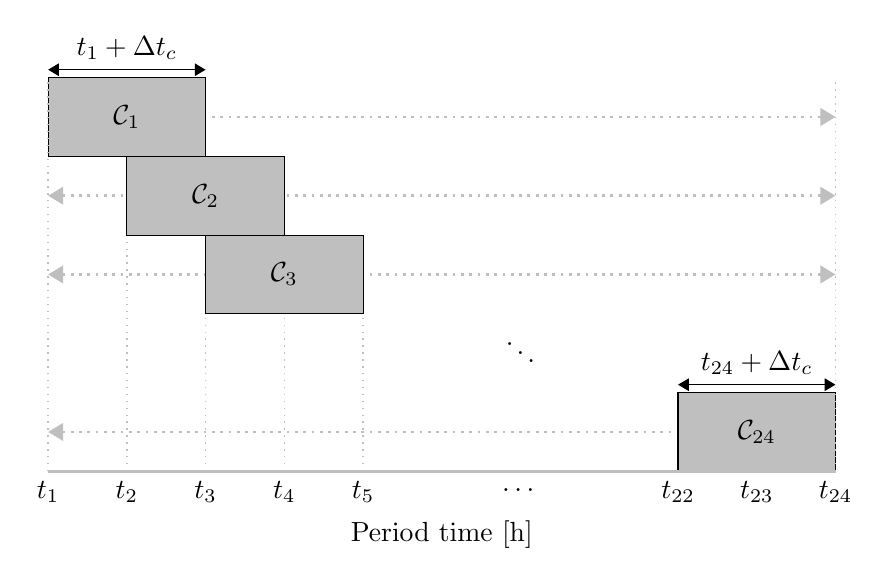
\begin{tikzpicture}[xscale=2, yscale=1, baseline]
    % \draw[help lines] (0,0) grid (5,5);

    %grid lines
    \draw [lightgray, dotted, line width=1, <->][Triangle-Triangle] 
            (0,4.5) -- (5,4.5);
    \draw [lightgray, dotted, line width=1, <->][Triangle-Triangle] 
            (0,3.5) -- (5,3.5);
    \draw [lightgray, dotted, line width=1, <->][Triangle-Triangle] 
            (0,2.5) -- (5,2.5);
    \draw [lightgray, dotted, line width=1, <->][Triangle-Triangle] 
            (0,0.5) -- (5,0.5);

    \draw [lightgray, dotted, line width=0.5] 
            (0.5,0) -- (0.5,3);
    \draw [lightgray, dotted, line width=0.5] 
            (1,0) -- (1,2);
    \draw [lightgray, dotted, line width=0.5] 
            (1.5,0) -- (1.5,2);
    \draw [lightgray, dotted, line width=0.5] 
            (2,0) -- (2,2);

    \node[below] at (3,2) {$\ddots$};

    % body
    \draw [fill=lightgray] (0,4) rectangle (1,5);
        \draw [black, line width=0.5, <->][Triangle-Triangle] 
            (0,5.1) -- (1,5.1);
        \node [above] at (0.5,5.1) {$t_{1} + \Delta t_{c}$};
            \node at (0.5,4.5) {$\mathcal{C}_{1}$};

    \draw [fill=lightgray] (0.5,3) rectangle (1.5,4);
        %\draw [black, line width=0.5, <->][Triangle-Triangle] 
        %   (1,4.1) -- (2,4.1);
        %\node [above] at (1.5,4) {$t_{2} + \Delta t_{c}$};
            \node at (1,3.5) {$\mathcal{C}_{2}$};

    \draw [fill=lightgray] (1,2) rectangle (2,3);
        %\draw [black, line width=0.5, <->][Triangle-Triangle]
        %    (2,3.1) -- (3,3.1);
        %\node [above] at (2.5,3) {$t_{3} + \Delta t_{c}$};
            \node at (1.5,2.5) {$\mathcal{C}_{3}$};
    % \draw [dotted, line width=1] (3,2) -- (4,1);

    \draw [fill=lightgray] (4,0) rectangle (5,1);
        \draw [black, line width=0.5, <->] [Triangle-Triangle] 
            (4,1.1) -- (5,1.1);
        \node [above] at (4.5,1.1) {$t_{24} + \Delta t_{c}$};
            \node at (4.5,0.5) {$\mathcal{C}_{24}$};

    %axis lines        
    \draw [lightgray, dotted, line width=0.5]  (0,0) -- (0,5);
    \draw [lightgray, dotted, line width=0.5]  (5,0) -- (5,5);
    \draw [lightgray, line width=1 ] (0,0) -- (5,0);
    %\draw [black, line width=1 ] (0,5.5) -- (5,5.5);

    % x labels
    \node[below] at (0,0) {$t_1$};
    \node[below] at (0.5,0) {$t_2$};
    \node[below] at (1,0) {$t_3$};
    \node[below] at (1.5,0) {$t_4$};
    \node[below] at (2,0) {$t_5$};
    \node[below] at (4,0) {$t_{22}$};
    \node[below] at (4.5,0) {$t_{23}$};
    \node[below] at (5,0) {$t_{24}$};
    \node[below] at (3,-0.1) {$\dotsc$};

    \node[below] at (2.5,-0.5) {$\text{Period time [h]}$};    
\end{tikzpicture}
    \caption{Set of contingencies.} 
    \label{fig:outages}
\end{figure}

Power outages or contingencies, typically caused by faults such as short circuits, can result from natural events, malfunctioning protective devices, or equipment failures. The EMS must be capable of maintaining system stability during such contingencies or load variations. During power outages, the microgrid circuits may isolate, supplying critical loads while non-essential loads are off.

This way, such failures in the main power grid can occur anytime, forcing the microgrid to operate in islanded mode. In this context,  the set $\mathcal{C}$ includes all the possibilities of occurrence of a contingency for a given hour. The model considers a set of 
24 contingencies that reflect all time intervals \{1, ..., 24\}, 
each potentially occurring at any hour within the 24-hour interval. 
Each contingency lasts for two hours ($\Delta t_c$), after which the microgrid reconnects to the grid, see Fig. \ref{fig:outages}.

\subsection{Mathematical model for the EMS}

The \gls{ems} mathematical model is formulated as a \gls{minlp} 
model, encompassing two objective functions and constraints related to the 
three-phase operation of the microgrid under different scenarios and 
contingencies. Subsection \ref{subsec:moop} discusses the solution method for 
\glspl{moop}. The main purpose of the \gls{ems} is to find the best solution, minimizing 
operational costs from the main grid and the \gls{ens} for \glspl{ev}. 
In sequence, a set of linearizations is used to transform the 
\gls{minlp} into a \gls{milp} model.  Details of the continuous and binary
decision variables used in this transformation can be found in 
\ref{appndx:piecewise}.

\subsubsection{Objective function 1}

The first objective function, given by \eqref{obj_1}, seeks to minimize the 
operational costs of the microgrid for a day-ahead scheduling. 
The first component refers to the cost of purchasing electricity 
from the main grid. The second component calculates the costs of the \gls{genset} 
operation, and the last one penalizes any load curtailment. All these
components are subject to the probability of a contingency occurring and the probability of each scenario occurring. 

\vspace{-15pt}
\begin{multline}\label{obj_1}
{f_{costs}} = \Delta t \sum_{s \in \mathcal{S}} \sum_{c \in \mathcal{C}}
    \Biggl\{ \mathit{Prob}_{s} \cdot \mathit{Prob}_{c} \cdot \Bigg[
        \sum_{i \in \mathcal{N}} 
        \sum_{f \in \mathcal{F}} 
        \sum_{t \in \mathcal{T}}  
\alpha_{t}^{\text{S}} P_{i,f,t,c,s}^{+\text{PCC}}  %\\
    + \sum_{n \in \mathcal{G}} 
    \sum_{t \in \mathcal{T}} 
\Big(P^{\text{G}}_{n,t,c,s} \cdot \alpha_{n}^{\text{G}} \cdot \mu_{n,t,c,s} \Big)  \\
    + \sum_{i \in \mathit{N}} 
    \sum_{f \in \mathit{F}}
    \sum_{t \in \mathit{T}}
   \alpha^{\text{C}} P_{i,f,t}^{\text{D}} 
        (1 - \chi_{i,t,c,s}) \Bigg] \Biggr\} 
\end{multline}
\vspace{-12pt}

\subsubsection{Objective function 2}

The second objective function, given by \eqref{obj_2}, aims to minimize the 
\gls{ens} to each \gls{ev} during the hours that coincide with their 
departure times.  This ensures that the \glspl{ev} receives sufficient charging, 
even for intervals of one or two hours, thereby guaranteeing their 
availability when needed by the \gls{ev} owner. The associated factor
$\omega_{r}$, represents the weight assigned to each \gls{ev}, further 
explanation is detailed in Section \ref{subsec:ev_fairness}.

\begin{equation}\label{obj_2}
{f_{ens}} = \sum_{\forall r,t | t=t_{d}} 
    \omega_{r} \left( \overline{{E}_{r}^{\mathrm{EV}}} - {E}_{r,t}^{\mathrm{EV}} \right)
\end{equation}

\subsubsection{Constraints related to the operation of three-phase distribution systems}

The three-phase unbalanced AC optimal power flow is described by 
(\ref{P_flow})–(\ref{bin_1}). 
Constraints (\ref{P_flow}) and (\ref{Q_flow}) 
ensure the active and reactive power balance, while constraints 
(\ref{P_losses}) and (\ref{Q_losses}) 
calculate the power losses, respectively. Note that the binary variable $\chi_{i,t,c,s}$ represents load curtailment, while the continuous variable $\psi_{i,t,c,s}$ sets a reduction in \gls{pv} generation.
Eq.~(\ref{V_drop}) calculates the voltage magnitude drop through the lines.
Voltage limits are guaranteed by (\ref{V_limit}), while (\ref{V_nom}) 
fixes the voltage magnitude at the PCC node. Constraint \ref{pcc_import} ensures that the net power at the \gls{pcc} equals the difference between imported and exported energy. The current magnitude flow is defined by (\ref{I}), and (\ref{pcc}) sets 
the substation capacity. Finally, \ref{bin_1} defines the binary nature of the load curtailment.

\vspace{-10pt}
\begin{multline}\label{P_flow}
    \hspace{-10pt}\sum_{ki\in \mathcal{L}} P_{ki,f,t,c,s} 
    - \sum_{ij\in \mathcal{L}} \Big(P_{ij,f,t,c,s} + 
    P^{\text{L}}_{ij,f,t,c,s} \Big) + 
    P^{+\text{PCC}}_{i,f,t,c,s} + %\\ 
    \!\!\sum_{n\in \mathcal{G} |i=L^G(n)}\!\!\!\!\!\!\! P^{\text{G}}_{n,f,t,c,s} + 
    P^\text{PV}_{i,f,t} \cdot \gamma^{\text{PV}}_{s} \cdot \psi_{i,t,c,s}
    = \\
    P^\text{D}_{i,f,t} \cdot \gamma^{\text{D}}_{s} \cdot \chi_{i,t,c,s}  + %\\ \!\!\!\!\!\!\!
    \!\!\!\!\!\sum_{m\in \mathcal{B} |i=L^B(m)}\!\!\!\!\! P^{\text{B}}_{m,t}\!  +
    \!\!\!\!\!\sum_{r\in \mathcal{V} |i=L^{\text{EV}}(r)}\!\!\!\!\!\!\! 
        P^{\text{\text{EV}+}}_{r,f,t}
    \quad  \forall \ i,f,t,c,s
\end{multline}
\vspace{-20pt}

\begin{multline}\label{Q_flow}
    \hspace{-10pt}\sum_{ki\in \mathcal{L}} Q_{ki,f,t,c,s} - 
    \sum_{ij\in \mathcal{L}} \Big(Q_{ij,f,t,c,s} + 
    Q^{\text{L}}_{ij,f,t,c,s} \Big) + 
    Q^\text{PCC}_{i,f,t,c,s} + %\\
    \!\!\!\sum_{n\in \mathcal{G} |i=L^G(n)}\!\!\!\! Q^{\text{G}}_{n,f,t,c,s} = 
    Q^\text{D}_{i,f,t} \cdot \gamma^{\text{D}}_{s} \cdot \chi_{i,t,c,s}  
    \\ \quad \forall \ i,f,t,c,s
\end{multline}
\vspace{-40pt}
  
\begin{multline}\label{P_losses}
    \hspace{-10pt}P^{\text{L}}_{ij,f,t,c,s} = %\\
    \sum_{h \in \mathcal{F}} 
        \frac{1}{V_{i,f,t,c,s}V_{i,h,t,c,s}}
    \bigg[ R'_{ij,f,h}\Big( P_{ij,h,t,c,s}P_{ij,f,t,c,s} + Q_{ij,h,t,c,s}Q_{ij,f,t,c,s}\Big)\\ 
    + X'_{ij,f,h} \Big( Q_{ij,h,t,c,s}P_{ij,f,t,c,s} - P_{ij,h,t,c,s}Q_{ij,f,t,c,s}\Big) \bigg] 
    \quad \forall \ ij,f,t,c,s
\end{multline}
\vspace{-30pt}
        
\begin{multline}\label{Q_losses}
    \hspace{-10pt}Q^{\text{L}}_{ij,f,t,c,s} = %\\
    \sum_{h \in \mathcal{F}} 
        \frac{1}{V_{i,f,t,c,s}V_{i,h,t,c,s}}
    \bigg[ R'_{ij,f,h}\Big(P_{ij,h,t,c,s}Q_{ij,f,t,c,s} - Q_{ij,h,t,c,s}P_{ij,f,t,c,s}\Big) \\ 
    + X'_{ij,f,h} \Big( P_{ij,h,t,c,s}P_{ij,f,t,c,s} + Q_{ij,h,t,c,s}Q_{ij,f,t,c,s}\Big)  \bigg] 
    \quad \forall \ ij,f,t,c,s
\end{multline}
\vspace{-30pt}

\begin{multline}\label{V_drop}
\hspace{-10pt}V^{\text{2}}_{i,f,t,c,s} - V^{\text{2}}_{j,f,t,c,s}  =
    2 \sum_{h \in \mathcal{F}} \left(  R'_{ij,f,h} P_{ij,h,t,c,s} +
    X'_{ij,f,h} Q_{ij,h,t,c,s} \right) - \\
    \frac{1}{V^{\text{2}}_{i,f,t,c,s}} 
    \left[\sum_{h \in \mathcal{F}}\left(R'_{ij,f,h}P_{ij,h,t,c,s} + 
    X'_{ij,f,h}Q_{ij,h,t,c,s}\right) \right]^2 -
    \\ \frac{1}{V^{\text{2}}_{i,f,t,c,s}}
    \left[\sum_{h \in \mathcal{F}}\left(R'_{ij,f,h}Q_{ij,h,t,c,s} - 
    X'_{ij,f,h}P_{ij,h,t,c,s}\right) \right]^2 
    \forall \ ij,f,t,c,s
\end{multline}
\vspace{-30pt}

\begin{flalign}\label{V_limit}
    &\underline{{V}}  \leq  V_{i,f,t,c,s}\leq  \overline{{V}}& \quad 
    \forall \ i,f,t,c,s &
\end{flalign}
\vspace{-40pt}

\begin{flalign}\label{V_nom}
    &V_{i,f,t,c,s} = {V}^{\text{nom}}&  \quad \forall \ i,f,t,c,s|_{i = \text{PCC}} &
\end{flalign}
\vspace{-40pt}

\begin{flalign}\label{pcc_import}
    &  P^\text{PCC}_{i,f,t,c,s} = P_{i,f,t,c,s}^{+\text{PCC}} - 
    P_{i,f,t,c,s}^{-\text{PCC}} & \quad  \forall \ i,f,t,c,s
\end{flalign}
\vspace{-40pt}
    
\begin{flalign}\label{I}
    &P^{2}_{ij,f,t,c,s} + Q^{2}_{ij,f,t,c,s} 
    \leq {V^{2}_{i,f,t,c,s}} \overline{I}_{ij}^2 & \quad \forall \ ij,f,t,c,s &
\end{flalign}
\vspace{-35pt}
    
\begin{flalign}\label{pcc}
    &\left( P_{i,f,t,c,s}^{\text{PCC}} \right)^2 + (Q_{i,f,t,c,s}^{\text{PCC}})^2 
    \leq (\overline{{S}^{\text{PCC}}_{i}})^2& \quad \forall \ i,f,t,c,s &
\end{flalign}
\vspace{-35pt}

\begin{flalign}\label{bin_1}
&\chi_{i,t,c,s} \in \{0, 1\} & \forall i,t,c,s 
\end{flalign}

\subsubsection{Constraints related to genset operation}

Constraints (\ref{P_G})–(\ref{QG_limits}) model the operation of the \gls{genset}. 
Equation (\ref{P_G}) and (\ref{Q_G}) define the total active and reactive 
power output for each phase, while (\ref{PG_limits}) and 
(\ref{QG_limits}) sets their limits, respectively. Finally, the binary variable \ref{bin_2} defines the operational state of the \gls{genset}.

\vspace{-6pt}
\begin{flalign}\label{P_G}
& P^{\text{G}}_{n,t,c,s} =  \sum_{f \in \mathcal{F}} P^{\text{G}}_{n,f,t,c,s}&
 \qquad \forall \ n,f,t,c,s 
\end{flalign}
\vspace{-30pt}

\begin{flalign}\label{Q_G}
& Q^{\text{G}}_{n,t,c,s} =  \sum_{f \in \mathcal{F}} Q^{\text{G}}_{n,f,t,c,s}&
 \qquad \forall \ n,f,t,c,s &
\end{flalign}
\vspace{-30pt}

\begin{flalign}\label{PG_limits}
& \underline{{P}^{\text{G}}_n} \cdot u_{n,t,c,s} \leq P^{\text{G}}_{n,t,c,s} 
\leq \overline{{P}^{\text{G}}_n}  \cdot u_{n,t,c,s}& \qquad 
  \forall \ n,t,c,s &
\end{flalign}
\vspace{-35pt}

\begin{flalign}\label{QG_limits}
& \underline{{Q}^{\text{G}}_n} \cdot u_{n,t,c,s} \leq Q^{\text{G}}_{n,t,c,s} 
\leq \overline{{Q}^{\text{G}}_n}  \cdot u_{n,t,c,s}& \qquad  \forall \ n,t,c,s &
\end{flalign}
\vspace{-35pt}

\begin{flalign} 
\label{bin_2}
&\mu_{n,t,c,s} \in \{0, 1\} & \forall n,t,c,s 
\end{flalign}

\subsubsection{Constraints related to islanded operation}

In the event of contingencies, constraints \eqref{pcc_1} and \eqref{pcc_2}
ensure the disconnection of the \gls{pcc}, which means no 
active or reactive power is supplied from the main grid during $t \geq c$ 
and $t \leq c + \Delta t_{0}$. 

\vspace{-3pt}
\begin{flalign}\label{pcc_1}
& P_{i,f,t,c,s}^{\text{PCC}} = 0& \qquad \forall i,f,t,c,s  | _{ t \geq c \ 
\wedge \ t \leq c + \Delta t_{0}} &
\end{flalign}
\vspace{-40pt}

\begin{flalign}\label{pcc_2}
& Q_{i,f,t,c,s}^{\text{PCC}} = 0& \qquad \forall i,f,t,c,s  | _{ t \geq c \ 
\wedge \ t \leq c + \Delta t_{0}} &
\end{flalign}

\subsubsection{Constraints related to BESS}

The operation of the \gls{bess} is modeled using 
\eqref{B_energy_1} - \eqref{B_lim_EB}. It is important to mention that the dispatch for the operation of the \gls{bess} is unique for all scenarios and contingencies.
Constraints \eqref{B_energy_1} and \eqref{B_energy_2} define the \gls{soc} of
the \gls{bess}, with \eqref{B_energy_1} based on the initial energy and
\eqref{B_energy_2} based on the energy stored in the previous period 
($ E_{m,t-1}^\text{B} $). Constraint \eqref{B_power} calculates the total 
input/output active power of the \gls{bess} in terms of charging 
$P^{\text{B}+}_{m,t}$ and discharging powers 
$P^{\text{B}-}_{m,t}$. 
Constraint \eqref{B_unimodality} ensures that the 
\gls{bess} do not charge and 
discharge simultaneously. Constraints \eqref{B_total_PBd} 
and \eqref{B_total_PBc} 
define the three-phase dis/charging power. Constraints 
\eqref{B_balance_1} 
and \eqref{B_balance_2} ensure a balanced operation.
Finally, constraints \eqref{B_lim_pch} - \eqref{B_lim_EB} establish the 
limits for the three-phase discharging/charging active power and energy based
on minimum and maximum capacities.

\vspace{-12pt}
\begin{flalign}\label{B_energy_1}
& E_{m,t}^\text{B}  = E_{m}^\text{B,\text{ini}}+ P^\text{B}_{m,t} \cdot \Delta t& 
\qquad \forall m,t | _{t = 1} &
\end{flalign}
\vspace{-37pt}

\begin{flalign}\label{B_energy_2}
& E_{m,t}^\text{B}  = E_{m,t-1}^\text{B}+ P^\text{B}_{m,t} \cdot \Delta t& 
\qquad \forall m, t | _{t>1} &
\end{flalign}
\vspace{-37pt}

\begin{flalign}\label{B_power}
& P_{m,t}^\text{B}  = P^\text{B+}_{m,t} \cdot \eta_{m}^\text{B} -
P_{m,t}^{\text{B}-} \cdot \frac{1}{\eta_{m}^\text{B}}& \qquad \forall m, t & 
\end{flalign}
\vspace{-37pt}

\begin{flalign}\label{B_unimodality}
& P^\text{B+}_{m,t} \cdot P_{m,t}^{\text{B}-} = 0& \qquad \forall m, t & 
\end{flalign}
\vspace{-37pt}

\begin{flalign}\label{B_total_PBd}
& P^{{\text{B}-}}_{m,t} =  \sum_{f \in \mathcal{F}} P^{{\text{B}-}}_{m,f,t}&
\qquad \forall m,t &
\end{flalign}
\vspace{-32pt}

\begin{flalign}\label{B_total_PBc}
& P^{\text{B+}}_{m,t} =  \sum_{f \in \mathcal{F}} P^{\text{B+}}_{m,f,t}&
\qquad  \forall m, t &
\end{flalign}
\vspace{-32pt}

\begin{flalign}\label{B_balance_1}
& P^{\text{B+}}_{m,f,t} =  P^{\text{B+}}_{m,h,t}& \qquad \forall m, f, h, t &
\end{flalign}
\vspace{-37pt}

\begin{flalign}\label{B_balance_2}
& P^{{\text{B}-}}_{m,f,t} =  P^{{\text{B}-}}_{m,h,t}& \qquad  \forall m, f, h, t&
\end{flalign}
\vspace{-37pt}

\begin{flalign}\label{B_lim_pch}
& 0 \leq P^{\text{B+}}_{m,t} \leq \overline{{P}^{\text{B}}_{m}} & %\cdot b^{+}_{m,t}&
\qquad  \forall m, t &
\end{flalign} 
\vspace{-37pt}

\begin{flalign}\label{B_lim_pdis}
& 0 \leq P^{{\text{B}-}}_{m,t} \leq \overline{{P}^{\text{B}}_{m}} &%\cdot b^{-}_{m,t} &
\qquad   \forall m, t &
\end{flalign}
\vspace{-37pt}

\begin{flalign}\label{B_lim_EB}
& \underline{{E}^{\text{B}}_{m}} \leq E^{\text{B}}_{m,t} \leq 
\overline{{E}^{\text{B}}_{m}}& \qquad  \forall m, t &
\end{flalign}

\subsubsection{Constraints related to EVs}

The operation of the \gls{evcs} for \glspl{ev} is modeled using 
\eqref{EV_1}–\eqref{EV_lim_EB}. These constraints consider only \gls{g2v}
operation and do not depend on the set of contingencies and scenarios. 
Constraints (\ref{EV_1}) and (\ref{EV_2}) define the \gls{soc} of the 
\glspl{ev}. The three-phase charging active power is described by 
(\ref{EV_total_PBc}), while (\ref{EV_balance_1}) ensures the balance of this
power. Equation (\ref{EV_out}) sets that \gls{ev} charging is restricted to the time range between time arrival ($t_{a}$) and time departure ($t_{d}$) of the EV. Finally, (\ref{EV_lim_pch}) and 
(\ref{EV_lim_EB}) set the limits for the three-phase charging power and
energy based on the \gls{ev}'s minimum and maximum capacities.

\vspace{-15pt}
\begin{flalign}\label{EV_1}
& E_{r,t}^\text{EV}  = E_{r}^\text{EV,\text{ini}}+ 
P^\text{EV}_{r,t} \cdot \eta_{r}^\text{EV} \cdot \Delta t&   \qquad 
\forall r,t | _{t = t_{a,r}} &
\end{flalign}
\vspace{-34pt}

\begin{flalign}\label{EV_2}
 & E_{r,t}^\text{EV}  = E_{r,t-1}^\text{EV} + 
 P^\text{EV}_{r,t} \cdot \eta_{r}^\text{EV} \cdot \Delta t&  \ \ \quad 
 \forall r, t  | _{ t \geq t_{a,r} \ \wedge \ t \leq t_{d,r}} &
\end{flalign}
\vspace{-34pt}

\begin{flalign}\label{EV_total_PBc}
& P^{\text{EV}}_{r,t} =  \sum_{f \in \mathcal{F}} P^{\text{EV}}_{r,f,t}&
 \qquad \forall r,t | _{ t \geq t_{a,r} \ \wedge \ t \leq t_{d,r}} &
\end{flalign}
\vspace{-30pt}

\begin{flalign}\label{EV_balance_1}
& P^{\text{EV}}_{r,f,t} =  P^{\text{EV}}_{r,h,t}& \qquad  
\forall r,f,h,t | _{t \geq t_{a,r} \ \wedge \ t \leq t_{d,r}} &
\end{flalign}
\vspace{-34pt}

\begin{flalign}\label{EV_out}
& P^{\text{EV}}_{r,f,t} = 0&  
\forall r,f,t | _{ t < t_{a,r} \ \vee \ t > t_{d,r}} & 
\end{flalign}
\vspace{-34pt}

\begin{flalign}\label{EV_lim_pch}
& 0 \leq P^{\text{EV}}_{r,t} \leq \overline{{P}^{\text{EV}}_{r}}&   \qquad \ 
\forall r, t | _{ t \geq t_{a,r} \ \wedge \ t \leq t_{d,r}} &
\end{flalign}
\vspace{-34pt}

\begin{flalign}\label{EV_lim_EB}
& \underline{{E}^{\text{EV}}_{r}} \leq E^{\text{EV}}_{r,t} \leq 
\overline{{E}^{\text{EV}}_{r}} &  \qquad 
\forall r, t | _{ t \geq t_{a,r} \ \wedge \ t \leq t_{d,r}} &
\end{flalign}

\subsection{Fairness in EV charging}\label{subsec:ev_fairness}

Fairness in \glspl{ev} charging ensures that all users receive equitable access to energy. It balances charging needs and prioritizes availability, regardless of initial battery state or time of connection, to minimize disparities in service provision. Thus, the following equations are designed to distribute energy between fairly \glspl{ev} when there isn’t enough to charge all EVs fully. A weighting method was defined based on each \gls{ev}'s available charging time and required energy. The equations also limit the amount of \gls{ens} to ensure that \glspl{ev} receive energy proportional to their needs.

Eqs.~\eqref{t_max} and \eqref{e_max} calculate the maximum availability time of EVs at the charging station, considering their arrival ($t_{a,r}$) and departure ($t_{d,r}$) times, and the maximum required energy of the EVs according to their capacity and initial energy. Eq.~\eqref{fairness_index} defines the fairness index associated with each EV, considering factors such as the initial SoC, the time available for charging, and the energy demand of each EV.
Two factors, $\alpha$ and $\beta$, both set to $0.5$, assign equal importance to time and energy in the calculation. 

\vspace{-10pt}
\begin{flalign}\label{t_max}
    & \overline{t} = \text{max} (t_{d,r} - t_{a,r} + 1) & \forall \  r \in \mathcal{V}
\end{flalign}
\vspace{-35pt}

\begin{flalign}\label{e_max}
    &\overline{E} = \text{max} (\overline{E_{r}^{\text{EV}}} - 
    E_{r}^\text{EV,\text{ini}}) &
    \forall \  r \in \mathcal{V}
\end{flalign}
\vspace{-35pt}

\begin{flalign}\label{fairness_index}
    &\omega_{r} = \alpha \frac{(t_{d,r} - t_{a,r} + 1)}{\overline{t}} + 
                    \beta \frac{(\overline{E_{r}^{\text{EV}}} - 
                    E_{r}^\text{EV,\text{ini}})}{\overline{E}} &
                    \forall \  r \in \mathcal{V}                  
\end{flalign}

Thus, the fairness indexes are applied in the objective function \eqref{obj_2}, which ensures that the weighted 
sum of \gls{ens} for the \glspl{ev} does not exceed a limit defined by 
set of $\varepsilon_{p}$ values (more details in Section \ref{subsec:moop}). This is crucial for 
ensuring fairness, as it allocates the energy shortfall between the 
\glspl{ev} based on their time and energy needs.


\subsection{Multi-objective optimization problem}\label{subsec:moop}

A \gls{moop} involves more than one objective function to be minimized or
maximized, where the answer is a set of solutions defining the best trade-off between the objectives. In this context, dominance determines the solution for the \gls{moop}. For instance, solution $x_1$  dominates $x_2$ if $x_1$ is no worse than $x_2$ in both objectives and strictly better than $x_2$ in at least one objective. If either of these conditions is violated, we have non-dominated solutions \cite{deb11}. In other words, the non-dominated solutions are those not dominated by any other solution. The boundary formed by these solutions is known as the Pareto-optimal front or optimal trade-off surface \cite{boyd2004}.

To solve the \gls{moop}, we employ the $\varepsilon$-constraint method. 
This technique is widely recognized for its simplicity and applicability in \gls{moop} \cite{chiandussi2012}. Introduced by \cite{haimes71}, this method involves keeping one objective function while restricting the other objectives as constraints within specific values. These values, known as the $\varepsilon$-vector, must be chosen within the minimum 
or maximum values of the constrained objective functions. 
In this problem, we select the first objective function \eqref{obj_1} as 
the main objective function, and consider the second objective 
function \eqref{obj_2} as a constraint. The modified problem is as follows:

\begin{equation}
    \left.
    \begin{aligned}
    \text{minimize} &\quad \text{$f_{costs}$}\\
    \text{subject to}&\quad \text{$f_{ens}$} \leq \text{$\varepsilon_{p}$},\\
    &\eqref{P_flow} - \eqref{bin_1}, \eqref{P_G}-\eqref{bin_2},\\
    &\eqref{pcc_1}-\eqref{pcc_2}, \eqref{B_energy_1}-\eqref{B_lim_EB},\\
    &\eqref{EV_1}-\eqref{EV_lim_EB} \\
    \end{aligned}
    \right\}
    \label{final_equation}
\end{equation}

The set of $\varepsilon_{p}$ values was chosen based on the storage capacity of
the EV batteries $\overline{E_{r}^{\text{EV}}}$. The minimum value of $0$ 
represents full charging for all EVs, while the maximum value, equal to the sum
of all capacities, represents no charging for any EV.

\section{EMS software architecture}\label{sec:architecture}

This section briefly describes the IoT-based EMS architecture developed in \cite{silva2023} and improved in the present work. We introduce the development of a new tab in the \gls{gui}, 
along with its corresponding database table, to set all the parameters 
associated with the \glspl{ev}.

\subsection{Backend}

The IoT-based \gls{ems} consists of 
five main modules: a stochastic \gls{edo} module, 
an \gls{api}, a database, a job scheduler (Cron), and a web-based \gls{gui}.

%\subsubsection{Economic dispatch optimizer (EDO)}

The main objective of the \gls{edo} module is to 
define the optimal day-ahead scheduling of \glspl{der} within the microgrid, 
including the charge/discharge of the \gls{bess}, \gls{pv},
and load curtailment, \gls{genset} dispatch, and \glspl{ev} charging.

The \gls{edo} module is triggered by the Cron module every 24 hours to
calculate the optimal dispatch for the next day. The results are stored in the
database tables and sent to the frontend of the IoT-based \gls{ems}.

Equation \eqref{final_equation} in Section \ref{subsec:moop} is solved 
using the solver CBC \cite{cbc} within this module. The \gls{edo} module was
implemented in Python using the \gls{pyomo} library \cite{bookpyomo, artpyomo}.

\begin{figure}
    \centering
    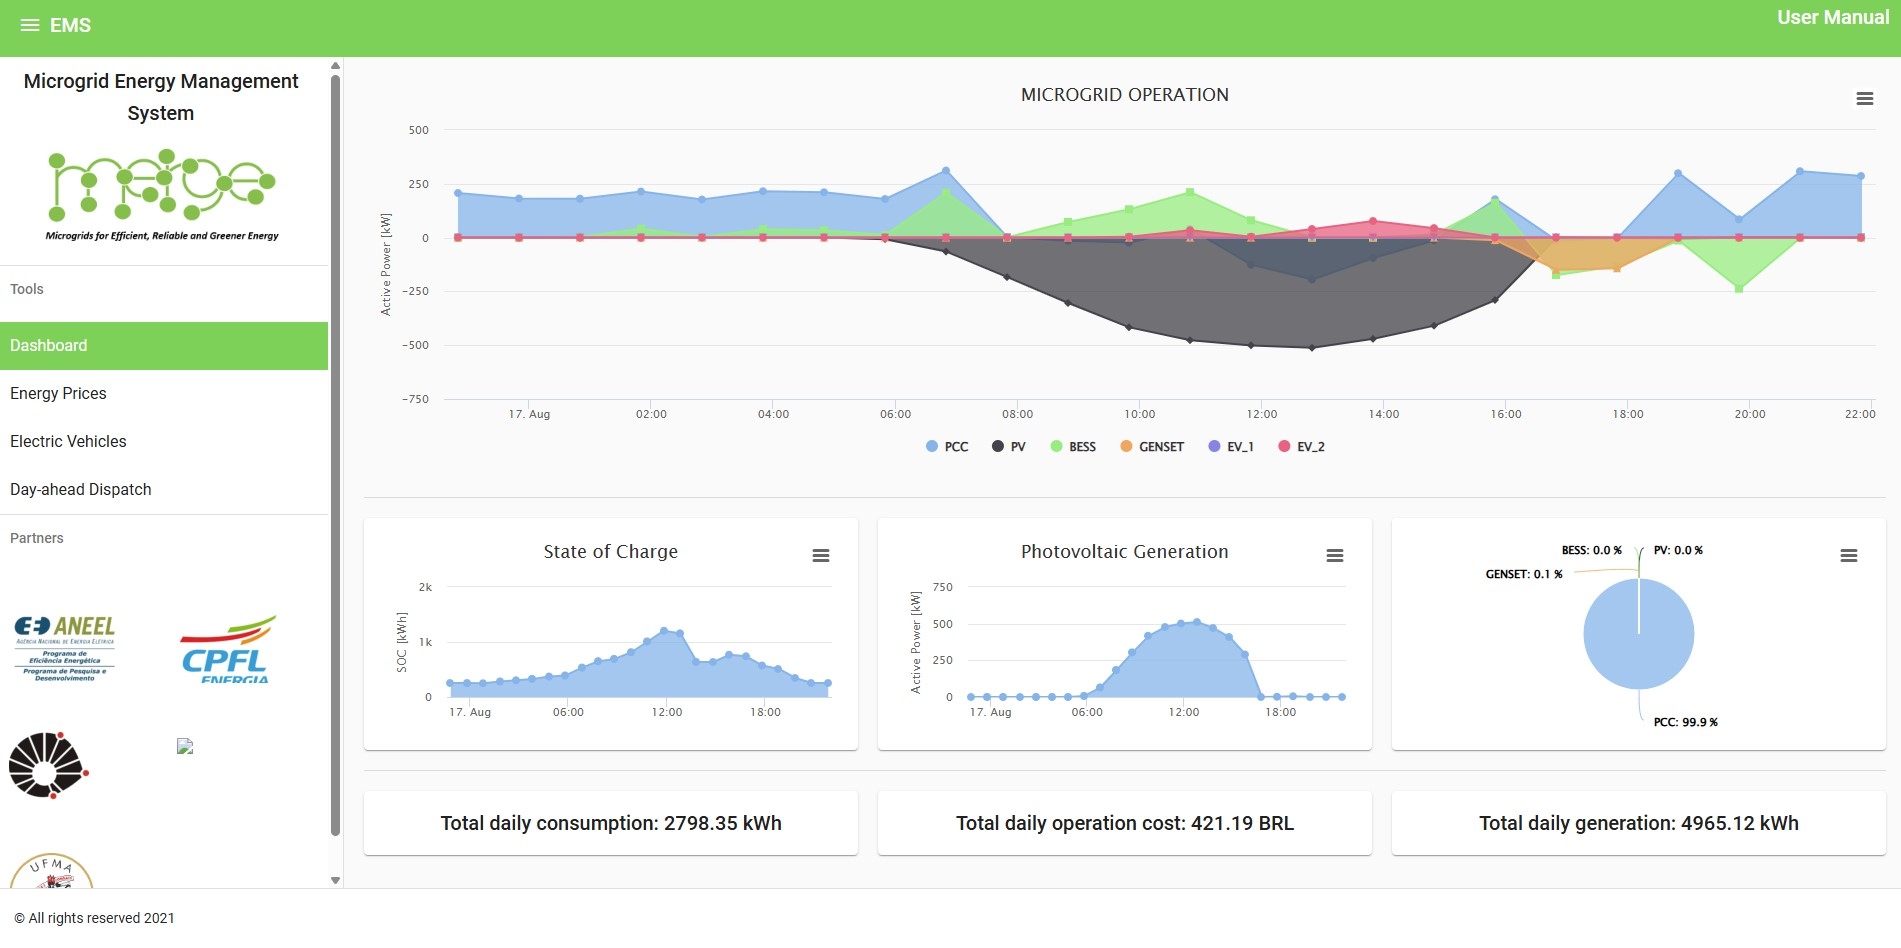
\includegraphics[width=\textwidth]{Figures/EMS/dashboard.jpg}
    \caption{GUI of the EMS - Frontend.}
    \label{fig:EMS_Frontend}
\end{figure}

\begin{figure}
    \centering
    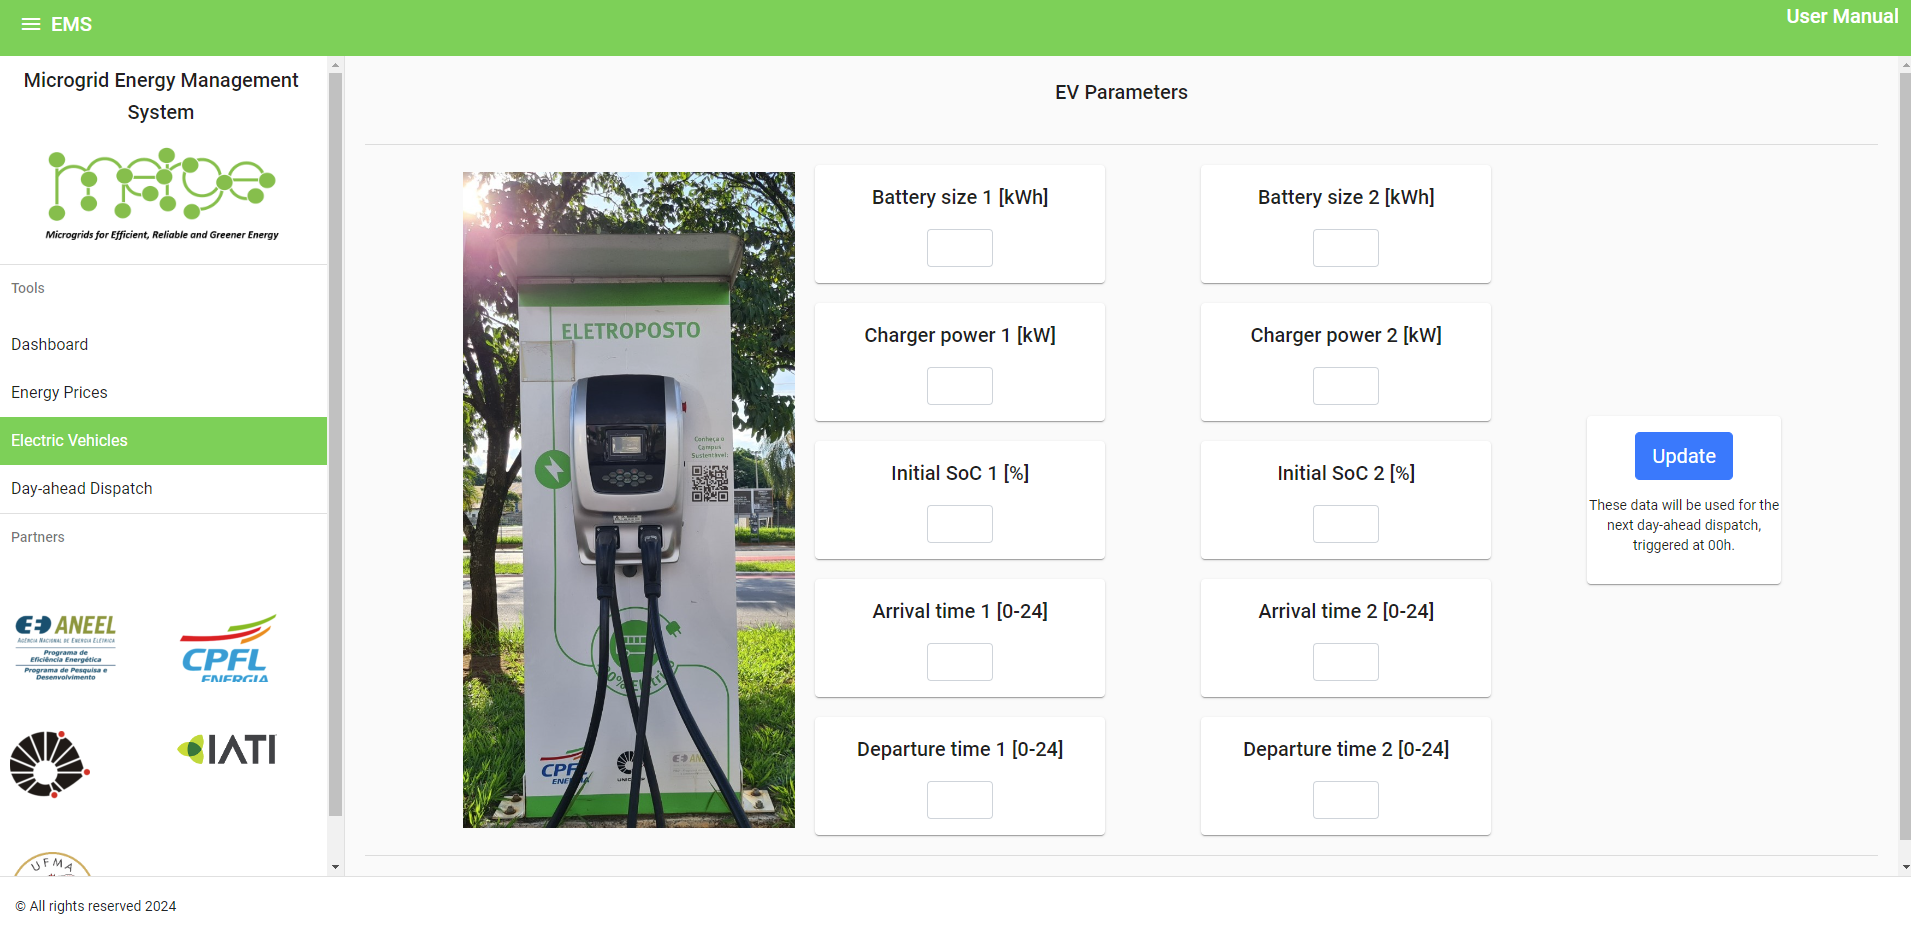
\includegraphics[width=\textwidth]{Figures/EMS/EVs.png}
    \caption{Electric vehicles tab - GUI of the EMS.}
    \label{fig:EMS_Frontend_ev}
\end{figure}

\subsection{Frontend}

The frontend of the IoT-based EMS is a user-friendly \gls{gui} accessible via
web browser, with various tabs for different functionalities.
The \glspl{ev} tab stands out as it was specifically 
developed for this work. The available tabs are:

\begin{itemize}
    \item \text{Dashboard}: The home screen displays real-time microgrid 
    operation data, including SOC of the BESS, PV power generation, and a pie 
    chart comparing energy sources. Daily consumption, operation cost, and 
    generation are also shown. See Fig. \ref{fig:EMS_Frontend}.
    \item \text{Electrical Vehicles}: Provides information on 
    arrival and departure times, power charging, and battery capacity for 
    \glspl{ev}. Fig. \ref{fig:EMS_Frontend_ev} shows the new \gls{ev} tab.
    \item \text{Energy Prices}: Users can configure hourly energy prices, 
    thermal generation (genset) costs, and load shedding costs. 
    Configured prices are sent to the database, and a graph displays the 
    changes. For this work, the energy prices were set by \cite{aneel}.
    \item \text{Day-ahead Dispatch}: Shows the dispatch defined by the \gls{edo}
    module for the next day. It includes \gls{bess} charge/discharge, load and \gls{pv} curtailment, \gls{ev} charge, and \gls{genset} dispatch. See Section \ref{sec:tests_results}.
\end{itemize}

\section{Tests and results}\label{sec:tests_results}

This section begins with describing the test system utilized to model the microgrid, followed by the algorithm development that solves the \gls{moop}. It then presents the Pareto curve and analyzes the solutions that were obtained. Next, a fairness analysis for \glspl{ev} is conducted. Finally, six case studies were addressed, and the results are discussed in detail.

\subsection{Test system}\label{sec:case_study}

The microgrid was simulated using the schematic editor of
Typhoon HIL 604 software \cite{typhoonhil_software} (see Fig. \ref{fig:Microgrid_Schematic}), with data from a 
three-phase AC microgrid deployed on the campus of \gls{unicamp}, 
São Paulo, Brazil. The model includes three-phase impedances and meters for each node. The final node is equipped with an \gls{evcs}. 
The time-of-use tariff, the energy purchase at peak hours (18:00 – 21:00h) is USD 0.254; for the shoulder hours (16:00 – 18:00 h, 21:00 – 22:00 h), it is USD 0.167; and for the off-peak hours (remaining hours), it is USD 0.116, according to the prices outlined in \cite{aneel}. The
microgrid parameters are detailed in Table \ref{tab:microgrid_parameters}.

\begin{figure*}[!t]
    \centering
    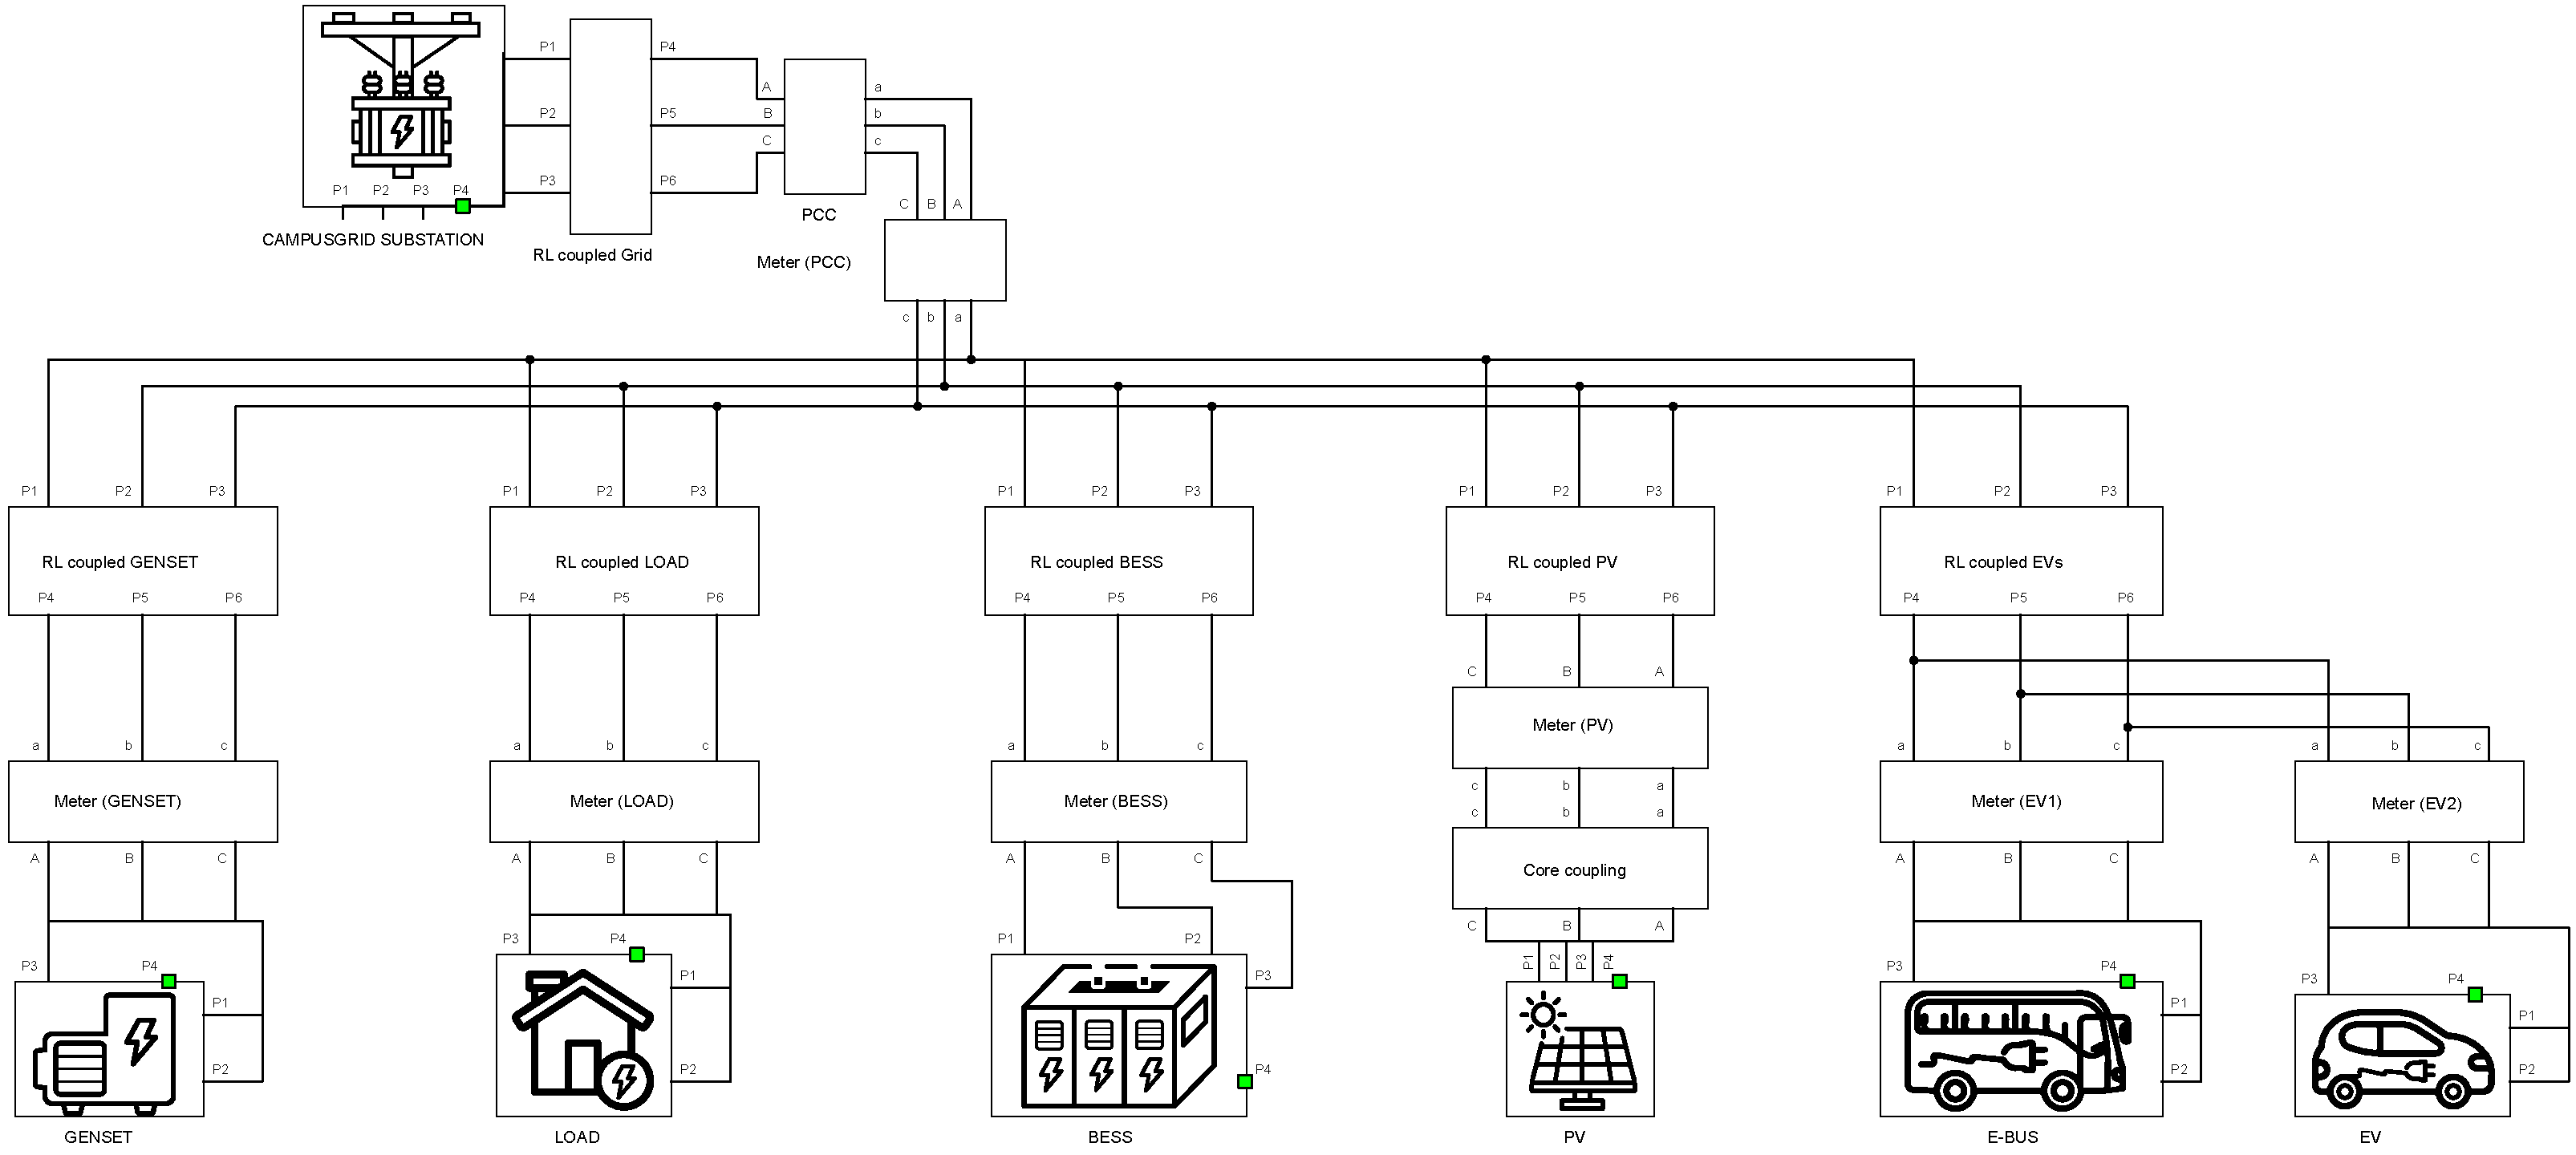
\includegraphics[width=0.98\textwidth]{Figures/schematic_HIL.pdf}
    \caption{Microgrid CAMPUSGRID schematic in Typhoon HIL 604.}
    \label{fig:Microgrid_Schematic}
\end{figure*}

\begin{table}[!t]
    \caption{Microgrid parameters.}
    \label{tab:microgrid_parameters} 
    \vspace{-15pt}
    \begin{center}
        \begin{threeparttable}
            \begin{tabular}{cccc}
            \hline
            Device & Parameter & Magnitude & Unit\\
            \hline
            \multirow{7}{*}{Grid}
            &$\overline{{V}}$, $\underline{{V}}$ 
                &\multicolumn{1}{l}{1.05 \quad 0.95} & [p.u.]\\
            &${S}^{\text{sub}}$ & 2375 & [kVA]\\
            &$\overline{{I}^{\text{PCC}}}$ & 1000 & [A]\\
            &${V}^{nom}$ & 11.9 & [kV]\\
            &${P}^{\text{D}}_{i}$ & 371 & [kW]\\
            &${Q}^{\text{D}}_{i}$ & 260 & [kvar]\\
            &${P}^{\text{PV}}_{i}$ & 736 & [kWp]\\
            \hline
            \multirow{3}{*}{Genset}
            &$\overline{{P}^{\text{G}}_{n}}$, $\underline{{P}^{\text{G}}_{n}}$ 
                &\multicolumn{1}{l}{150 \quad 0} & [kW]\\
            &$\overline{{Q}^{\text{G}}_{n}}$ , $\underline{{Q}^{\text{G}}_{n}}$
                &\multicolumn{1}{l}{150 \quad -150}&[kvar]\\
            &$\alpha_{n}^{\text{G}}$ &30&[m.u.]\\
            \hline
            \multirow{4}{*}{BESS}
            &$\overline{{E}^{\text{B}}_{m}}$, $\underline{{E}^{\text{B}}_{m}}$ 
                &\multicolumn{1}{l}{1275 \quad 260} & [kWh]\\
            &$\eta^{\text{B}}$ &95&[\%]\\
            &${E}^{\text{B}_{0}}_{m}$ &260&[kWh]\\
            &$\overline{{P}^{\text{B}}_{m}}$ &1000&[kW]\\
            \hline
            \multirow{4}{*}{E-Bus}
            &$\overline{{E}^{\text{EV}}_{r}}$, $\underline{{E}^{\text{EV}}_{r}}$ 
                &\multicolumn{1}{l}{324 \quad 64.8} & [kWh]\\
            &$\eta^{\text{EV}}$ & 95 & [\%]\\
            &${E}^{\text{EV}_{0}}_{r}$ & 64.8 & [kWh]\\
            &$\overline{{P}^{\text{EV}}_{r}}$ & 80 & [kW]\\
            \hline
            \multirow{4}{*}{EV}
            &$\overline{{E}^{\text{EV}}_{r}}$, $\underline{{E}^{\text{EV}}_{r}}$ 
                &\multicolumn{1}{l}{108 \quad 21.6} & [kWh]\\
            &$\eta^{\text{EV}}$ & 95 & [\%]\\
            &${E}^{\text{EV}_{0}}_{r}$ & 21.6 & [kWh]\\
            &$\overline{{P}^{\text{EV}}_{r}}$ & 11 & [kW]\\
            \hline
            \end{tabular}
        \end{threeparttable}
    \end{center}
\end{table}

The \gls{evcs} offers both slow charging (40kW) and fast charging (80kW) \cite{zaneti2022}. 
Considering the charging power offered by the microgrid's \gls{evcs}, fast charging was 
applied for the E-bus ($\overline{{P}^{\text{EV}}_{r}}$ = 80 kW) and for the EV ($\overline{{P}^{\text{EV}}_{r}}$ = 11 kW), as this aligns with the
power specifications of the EV \cite{byd_tan}. 
%
The E-bus is used to transport students throughout the day within the \gls{unicamp} 
campus, while the \gls{ev} is employed for campus security during nighttime. 
Therefore, the E-bus arrives and departs from the \gls{evcs} between 1:00 and 7:00 hours, 
while the \gls{ev} charges from 8:00 to 16:00 hours, following the schedule optimized 
for \gls{ev} charging as outlined in \cite{zaneti2022}. 

\subsection{Multi-objective optimization analysis}

Algorithm \ref{alg:e_constraint_method} was applied to solve 
equation \eqref{final_equation} from subsection \ref{subsec:moop}. Using the $\varepsilon$-Constraint method, the algorithm generated 
the Pareto front by solving constrained problem with varying 
$\varepsilon_{p}$ values in one objective while optimizing 
the other. This approach considered nine scenarios and two 
contingencies at 08:00 and 16:00 hours, storing non-dominated 
solutions to construct the Pareto front. Moreover, the arrival and 
departure times ($t_a$, $t_d$) 
at the charging station are set from 1:00 to 7:00 hours for E-bus and 
from 8:00 to 16:00 hours for \gls{ev}. 
As a result, obtains a set of non-dominated solutions, forming the 
Pareto front, as shown in Fig. \ref{fig:pareto_front}.

\begin{algorithm}
    \caption{$\varepsilon$-Constraint Method for \gls{moop}}
    \label{alg:e_constraint_method}
    \SetAlgoLined
    \KwData{Parameters of the \gls{moop}, including scenarios and contingencies}
    % \KwResult{Pareto front}
    % \BlankLine
    \textbf{Initialize:} 
    Set of $\varepsilon_{p}$ values\;
    % \BlankLine
    % \While{MOOP problem is feasible}{
    %     \For{$\varepsilon_{p}$ value}{
    %         \textbf{Solve:} {\eqref{final_equation}}\;
    % }}
    % \While{MOOP problem is feasible}{
        \For{each $\varepsilon_{p}$ value in the set}{
            \textbf{Solve:} {\eqref{final_equation}}\;
            \textbf{Store:} Non-dominated solutions\;
    }% }}
    % \BlankLine
    \textbf{Generate} Pareto front\;
    % \textbf{Measure:} Euclidean distance to the ideal point\;
    % \textbf{Compute:} The centroid of the Pareto front\;
\end{algorithm}

\begin{figure}
    \centering
    \tikzstyle{every pin}=[
    fill=white,
    draw=gray,
    font=\footnotesize]
    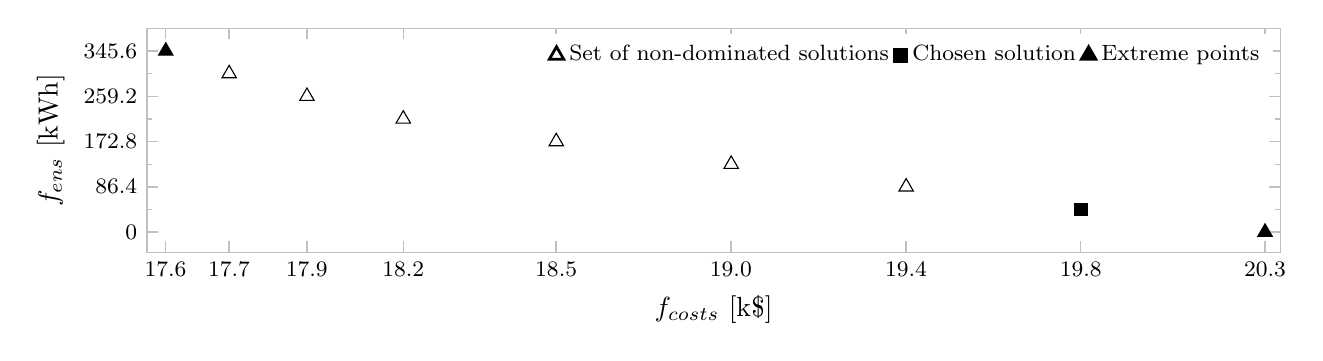
\begin{tikzpicture}
    \begin{axis}[
        %width=240pt,
        % height = 140pt,
        % x dir = reverse,
        y post scale = 0.5,
        x post scale = 2.1,
        xlabel={$f_{costs}$ [k\$]},
        xlabel near ticks,
        % axis x line = bottom,
        % axis line shift = 10pt,
        ylabel={$f_{ens}$ [kWh]},
        ylabel near ticks,
        % axis y line = left,
        % axis line style={|-stealth},
        % axis x discontinuity=crunch,
        tick style = {line width = 0.5, color = lightgray, 
            major tick length=4pt,minor tick length=2pt, 
            minor y tick num =1, xtick = {
            17645, 
            17799,
            17988,
            18222,
            18593,
            19017,
            19442,
            19866,
            20313}
            },
        xticklabels = {
            17.6,
            17.7,
            17.9,
            18.2,
            18.5,
            19.0,
            19.4,
            19.8,
            20.3
            },
        tick label style = {font=\footnotesize, ytick distance=86.4
            },
        xtick align = {inside},
        ytick align = {inside},
        % extra x ticks={10926.93},
        %extra x tick labels={10926.93},
        % label style = {font=\small},
        % legend style = {font=\footnotesize, at={(0.5,1.05)},    
        %     anchor=south, legend cell align=left, line width=0.5pt, 
        %     draw=lightgray, legend columns = 2}
        legend style = {font=\footnotesize, at={(0.995,0.98)},    
            anchor= north east, legend cell align=center, line width=1pt, 
            draw = none, legend columns = 3},
        ymax=388.8,
        xmin=17600, xmax=20350,
        % enlarge x limits=0.05,
        axis line style = {line width = 0.5pt, lightgray},
        scaled ticks=false
        ]

    
     % Set of non-dominated solutions 
    \addplot[mark = triangle, only marks, mark size = 3pt,
    black] 
    coordinates {

        (17799.57	,302.4)
        (17988.30	,259.2)
        (18222.13	,216)
        (18593.29	,172.8)
        (19017.81	,129.6)
        (19442.34	,86.4)
        % (19866.86	,43.2)
              
        };
    \addlegendentry{Set of non-dominated solutions}
    
    % Centroid
    \addplot [mark size = 2.2pt, only marks, mark = square*]
        coordinates {
        (19866.86	,43.2)
        };
    \addlegendentry{Chosen solution}

    \addplot [mark size = 3pt, only marks, mark = triangle*]
        coordinates {
        (17645.70	,345.6)
        (20313.20	,0)
        };
    \addlegendentry{Extreme points}
    % \node [coordinate, pin=above right:{Centroid}] at
    %     (axis cs: 13863.73, 259.2 ) {};
    % \node [coordinate, pin=above right:{Ideal Point}] at
    %     (axis cs: 10926.93, 0) {};
    \end{axis}
\end{tikzpicture}
    \vspace{-8pt}
    \caption{Pareto front}
    \label{fig:pareto_front}
\end{figure}


From the Pareto front, we highlight two extreme points. The first extreme 
point (upper left) represents the solution with the maximum value of
$f_{ens} = 345.6$ kWh and the minimum value of $f_{costs} = 17,645$ \$. The second 
extreme point (lower right) shows the solution with the minimum value 
of $f_{ens} = 0$ kWh and the maximum value of $f_{costs} = 20,313$ \$. Each of these points is discussed in detail in the following subsections.

To analyze these points individually, we focus on the dispatch of the \gls{bess} and \gls{ev}. 
In Fig. \ref{fig:first_extreme_point}, the \gls{bess} begins charging during the first
contingency and discharges during the second, while no \glspl{ev} are dispatched. This occurs because, with $\varepsilon_{p} = 345.6$ kWh, the \gls{edo} refrains from allocating charging to either \gls{ev}. As a result, priority is given to minimizing $f_{costs}$, yielding the lowest 
cost for the microgrid.

In the second extreme point, shown in Fig. \ref{fig:second_extreme_point}, the 
\gls{bess} charges similarly to the previous case; however, both \glspl{ev} are dispatched. 
At this point, $\varepsilon_{p} = 0$ kWh represents the minimum $f_{ens}$, indicating that 
both \glspl{ev} must fully charge. Consequently, this increased energy demand results in higher energy purchases, primarily for charging the E-bus, while the other \gls{ev} utilizes the microgrid’s \gls{pv} generation.

A $\varepsilon_{p} = 43.2$ kWh is selected to optimize costs, 
representing nearly 500\$ in savings for the microgrid’s operation. Notably, with \gls{moop} framework, all solutions obtained are optimal, allowing for selection flexibility to support microgrid decision-making. This analysis represents one of the key contributions highlighted in this work.


\begin{figure}
    \centering
    \begin{tikzpicture}
    \begin{axis}[ybar stacked,
        xlabel={Period time [h]},
        ylabel={Active power [kW]},
        ylabel near ticks,
        xlabel near ticks,
        bar width=4pt,
        tick style = {line width = 0.5, color = lightgray, 
            major tick length=4pt,minor tick length=2pt,
            minor x tick num = 3, minor y tick num =1},
        tick label style = {font=\footnotesize, xtick distance=4, ytick distance=100,
            xticklabels={01:00, 01:00, 04:00, 08:00, 12:00, 16:00, 20:00 }},
        legend style = {font=\footnotesize, at={(0.99,0.98)}, 
            legend cell align=left, line width=0.5pt, draw=lightgray},
        legend entries={BESS,E-BUS,EV},
        ymin=-350, ymax=250,
        xmin=0, xmax=25,
        axis line style = {lightgray, line width = 0.5pt},
        cycle multi list={
        lightgray, gray, black\nextlist
        fill
        }
        ]

        \addplot table 
        [col sep=comma, x = h,y=P_BESS] {./Data/firs_point.dat};
        \addplot table
        [col sep=comma, x = h, y=P_EV_1] {./Data/firs_point.dat};
        \addplot table
        [col sep=comma, x = h,y=P_EV_2] {./Data/firs_point.dat};

    \end{axis}
\end{tikzpicture}
    \caption{Dispatch of the first extreme point}
    \label{fig:first_extreme_point}
\end{figure}

\begin{figure}[h!]
    \centering
    \begin{tikzpicture}
    \begin{axis}[ybar stacked,
        xlabel={Period time [h]},
        ylabel={Active power [kW]},
        ylabel near ticks,
        xlabel near ticks,
        bar width=4pt,
        tick style = {line width = 0.5, color = lightgray, 
            major tick length=4pt,minor tick length=2pt,
            minor x tick num = 3, minor y tick num =1},
        tick label style = {font=\footnotesize, xtick distance=4, ytick distance=100,
            xticklabels={01:00, 01:00, 04:00, 08:00, 12:00, 16:00, 20:00 }},
        legend style = {font=\footnotesize, at={(0.99,0.98)}, 
            legend cell align=left, line width=0.5pt, draw=lightgray},
        legend entries={BESS,E-BUS,EV},
        ymin=-350, ymax=250,
        xmin=0, xmax=25,
        axis line style = {lightgray, line width = 0.5pt},
        cycle multi list={
        lightgray, gray, black\nextlist
        fill
        }
        ]

        \addplot table 
        [col sep=comma, x = h, y=P_BESS] {./Data/second_point.dat};
        \addplot table
        [col sep=comma, x = h, y=P_EV_1] {./Data/second_point.dat};
        \addplot table
        [col sep=comma, x = h, y=P_EV_2] {./Data/second_point.dat};
        
    \end{axis}
\end{tikzpicture}
    \caption{Dispatch of the second extreme point}
    \label{fig:second_extreme_point}
\end{figure}

\subsection{Fairness EVs analysis}\label{subsec:ev_fairness_analysis}

Fairness analyses are conducted based on the selected solution from the Pareto curve, with $\varepsilon_{p} = 43.2$ kWh. Various parameter combinations for \glspl{ev} management were tested. 
Table \ref{tab:fairness_analysis} presents results, considering energy capacity ($\overline{{E}^{\text{EV}}_{r}}$), state of charge (\gls{soc}), arrival and departure times, EV availability time
($t_{disp}$), weights, and required energy at the time of departure 
$(E^{\text{EV}}_{r,t|t={t_d}})$. Below is a detailed analysis of each case:

\begin{itemize}
    \item \textbf{Case I:} This case base evaluates two E-buses that have identical energy demand \linebreak
    (324\,kWh), SoC of 20\%, 
    and available charging time of 7 hours. Since all parameters are the same, both buses are 
    assigned equal weights (0.5). However, the first bus receives 280.8\,kWh, while the 
    second bus is fully charged at 324\,kWh. This difference arises from the adoption of the 
    $\varepsilon_{p} = 43.2$ kWh, which balances the system and helps serve as a reference for the subsequent cases.

    \item \textbf{Case II - Different energy capacity:} In this case, the arrival and departure times 
    and initial SoC remain the same; however, the E-bus has a larger capacity (324 kWh) than the EV (108 kWh). Consequently, the E-bus is assigned a higher weight of 0.62, compared to 0.38 for the EV, prioritizing its greater energy requirements. As a result, the E-bus receives 280.8 kWh, slightly below its total demand, while the EV is fully charged at 108 kWh. The system maintains fairness by prioritizing the E-bus due to its higher energy demand.

    \item \textbf{Case III - Different SoC levels:} In this scenario, two E-buses, one with a 60\% SoC and the other with a 20\% SoC, both have 7 hours of available charging time. The bus with the lower SoC (20\%) is assigned a higher weight of 0.58, compared to 0.42 for the bus at 60\%. Despite their initial SoC differences, both buses receive the same energy (302.4 kWh), demonstrating how the system balances energy needs and available time to promote fairness.

    \item \textbf{Case IV - Different charging times:} Here, two E-buses have the same energy demand 
    (324 kWh) and SoC (20\%), but different available charging times: one has 5 hours 
    and the other only 3 hours. The bus with more charging time is given a higher 
    weight (0.56) than the other (0.44). As a result, the bus with more time gets 
    312 kWh, while the other receives 292.8 kWh, demonstrating that the system prioritizes 
    those with more available charging time.

    \item \textbf{Case V - Complex case:} In this final case, all parameters vary. 
    The E-bus has a higher capacity (324 kWh vs. 108 kWh), a higher initial 
    SoC (50\% vs. 30\%), but less available charging time (4 hours vs. 7 hours). 
    The E-bus receives 283.25 kWh, while the EV gets almost all its required energy 
    (105.55 kWh). This case shows a balanced energy distribution, with a slight 
    preference for the E-bus due to its higher capacity and demand.
\end{itemize}

\begin{table*}[t!]
    \caption{EVs fairness analysis.}
    \label{tab:fairness_analysis}
    \vspace{-15pt}
    \begin{center}
        \begin{threeparttable}
            \begin{tabular}{ccccccccc}
            \hline
                &Device & $\overline{{E}^{\text{EV}}_{r}}$ [kWh]& \gls{soc}[\%] 
                    & $t_{a}$ [h]& $t_{d}$[h] & $t_{disp}$[h] & Weights 
                    & $E^{\text{EV}}_{r,t|t={t_{d}}}$ [kWh] \\
            \hline
                \multirow{2}{*}{Case I}
                & E-bus&324&20& 1 & 7 & 7 & 0.5 & 280.8\\
                & E-bus&324&20& 9 & 15 & 7 & 0.5 & 324\\
            \hline
                \multirow{2}{*}{Case II}
                & E-bus&324&40& 1 & 7 & 7 & 0.62 & 280.8\\
                & EV&108&40& 9 & 15 & 7 & 0.38 & 108\\
            \hline
                \multirow{2}{*}{Case III}
                & E-bus&324&60& 1 & 7 & 7 & 0.42 & 302.4\\
                & E-bus&324&20& 1 & 7 & 7 & 0.58 & 302.4\\
            \hline
                \multirow{2}{*}{Case IV}
                & E-bus&324&20& 1 & 5 & 5 & 0.56  & 312\\
                & E-bus&324&20& 13 & 15 & 3 & 0.44 &292.8\\
            \hline
                \multirow{2}{*}{Case V}
                & E-bus&324&50& 11 & 14 & 4 & 0.52 & 283.25\\
                & EV&108&30& 9 & 15 & 7 &  0.48& 105.55\\
            \hline
            \end{tabular}
        \end{threeparttable}
    \end{center}
\end{table*}

Overall, the proposed method ensures fair energy distribution by considering both the availability time of EVs and your energy needs.
The weighting system helps balance these factors, ensuring no vehicle is unfairly treated based
on arrival time, SoC, or charging needs. Vehicles with greater needs or more
available charging time receive slightly more energy. This fairness approach ensures optimal 
energy distribution even when resources are limited.

\subsection{Microgrid Operation Results: Case Studies and Analysis}\label{subsec:case_studies}

This section presents the operation of the microgrid using the IoT-based EMS. To conduct these case studies, the parameters from 
Table \ref{tab:microgrid_parameters} were applied in the \gls{edo} and 
the schematic editor of Typhoon HIL 604. Consequently, the results were also reflected in the GUI. 
It is important to highlight that the \gls{moop} chosen solution with 
a $\varepsilon_{p} = 43.2$ kWh was applied for these cases. Thus, the six case studies are presented as follows:

\begin{itemize}
    \item Case I: Without contingencies and no inclusion of \glspl{ev}.
    \item Case II: Contingency at 08:00 hours without \glspl{ev}.
    \item Case III: Without contingencies, including \glspl{ev}.
    \item Case IV: Contingency at 08:00 hours with  \glspl{ev}. 
    \item Case V: Contingency at 16:00 hours with \glspl{ev}.
    \item Case VI: Contingencies at 08:00 and 16:00 hours with \glspl{ev}. 

\end{itemize}

\subsubsection{Results}\label{subsec:results}

For each case, the stochastic \gls{edo} determines
the optimal day-ahead dispatch for \gls{der}s of the microgrid, considering the nine scenarios presented in Section~\ref{sec:uncertainty_set}. Consequently, the dispatch results 
for \gls{bess}, \gls{genset}, \gls{pv} reduction, and \glspl{ev} 
are shown in Fig. \ref{fig:bess_dispatch} to 
Fig. \ref{fig:genset_genset_dispatch}. Additionally, the 24-hour operation of 
the microgrid is illustrated in Fig. \ref{fig:microgrid_operation}.


\begin{figure*}[!t]
    \centering
    \subfloat[Case I: Without contingencies.]{
        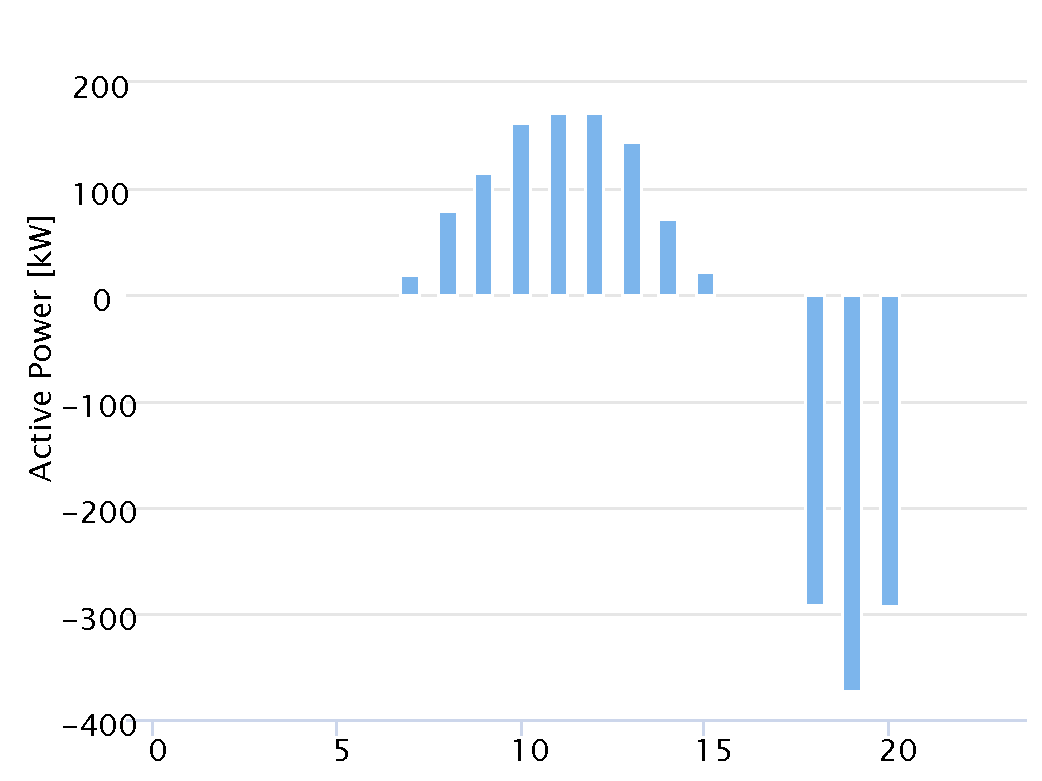
\includegraphics[width=0.45\textwidth]{Figures/1_case/bess-dispatch.pdf}
        \label{fig:case_I_bess_dispatch}
    }
    \subfloat[Case II: Contingency at 08:00 h.]{
        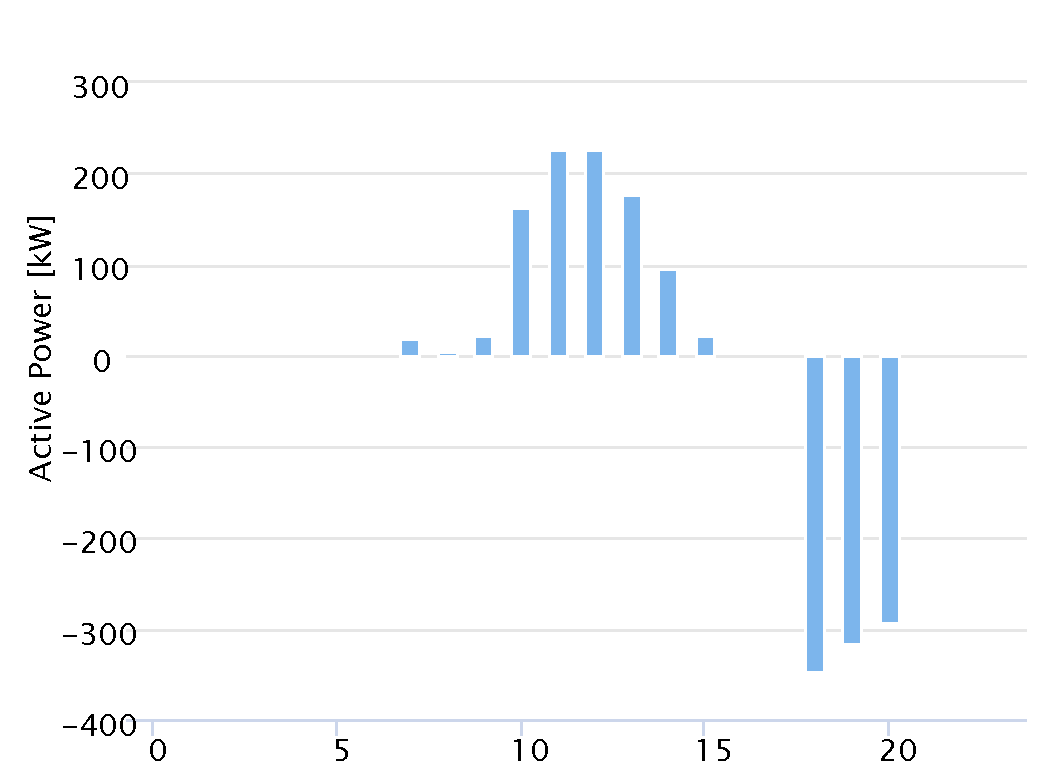
\includegraphics[width=0.45\textwidth]{Figures/2_case/bess-dispatch.pdf}
        \label{fig:case_II_bess_dispatch}
    }
    \vfill
    \subfloat[Case III: Without contingencies, including \glspl{ev}.]{
        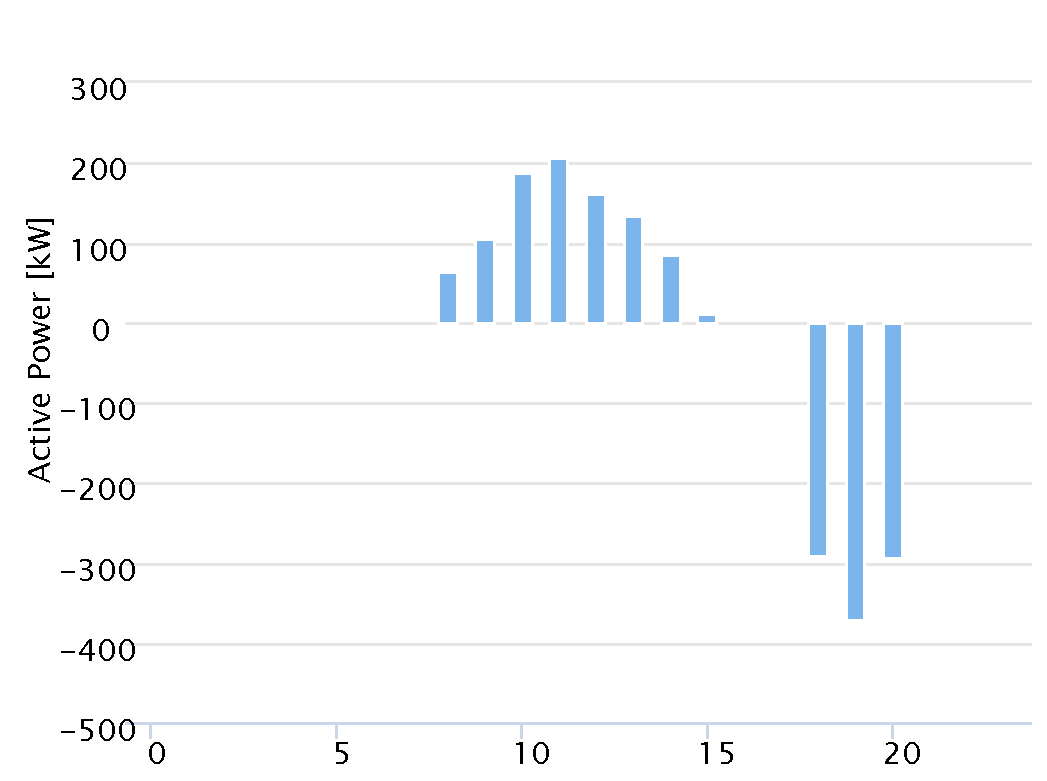
\includegraphics[width=0.45\textwidth]{Figures/3_case/bess-dispatch.pdf}
        \label{fig:case_III_bess_dispatch}
    }
    \subfloat[Case IV: Contingency at 08:00 h with \glspl{ev}.]{
        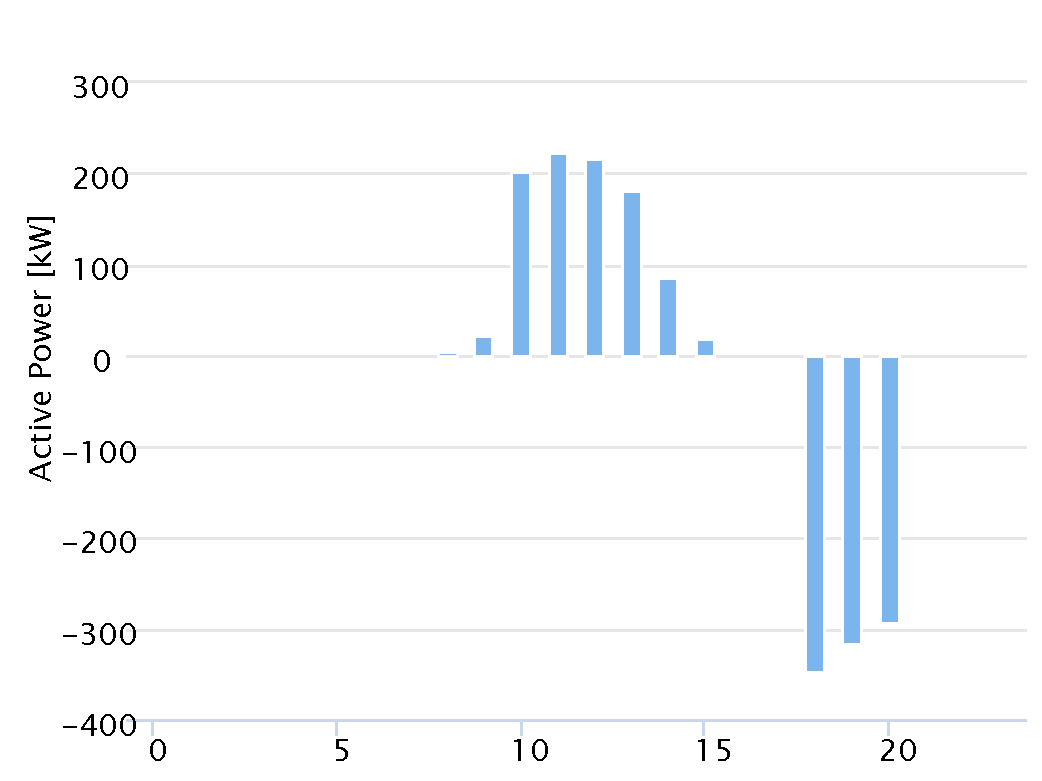
\includegraphics[width=0.45\textwidth]{Figures/4_case/bess-dispatch.pdf}
        \label{fig:case_IV_bess_dispatch}
    }
    \vfill
    \subfloat[Case V: Contingency at 16:00 h with \glspl{ev}.]{
        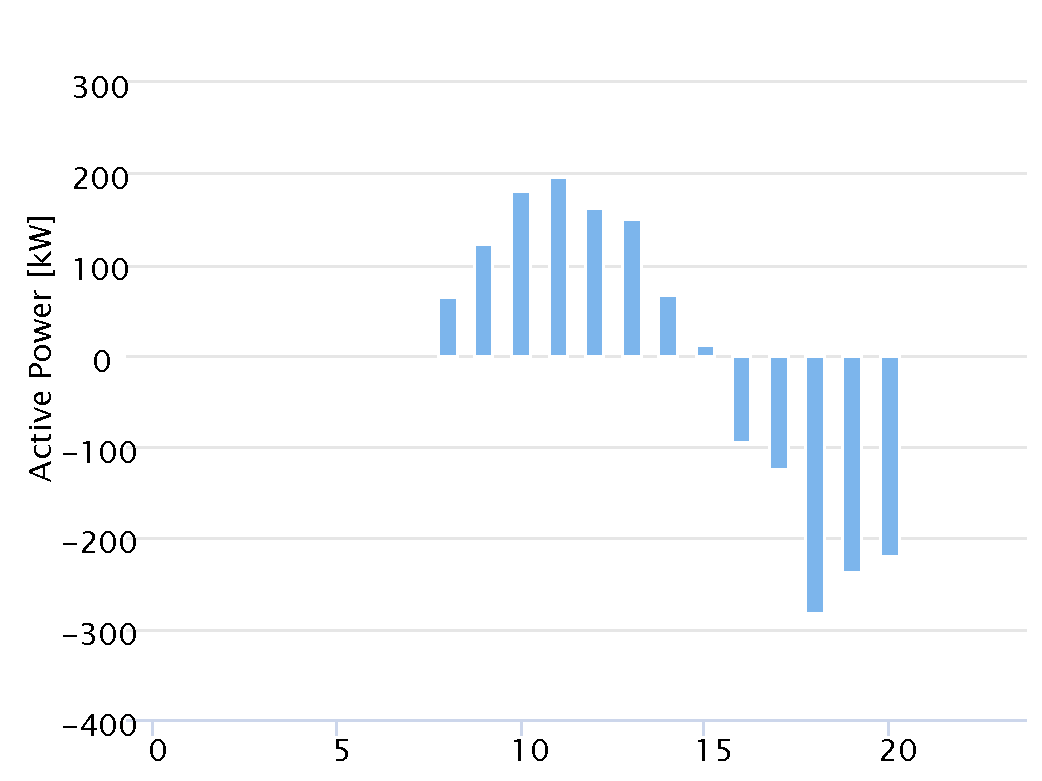
\includegraphics[width=0.45\textwidth]{Figures/5_case/bess-dispatch.pdf}
        \label{fig:case_V_bess_dispatch}
    }
    \subfloat[Case VI: Contingencies at 08:00 and 16:00 hours with \glspl{ev}.]{
        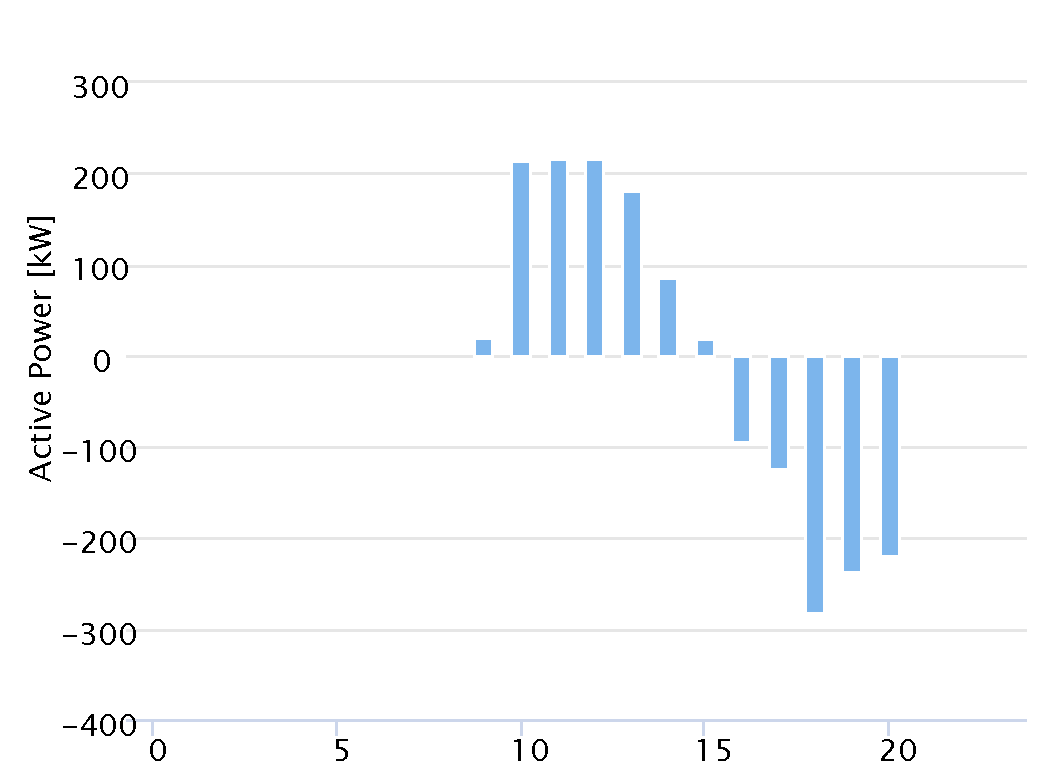
\includegraphics[width=0.45\textwidth]{Figures/6_case/bess-dispatch.pdf}
        \label{fig:case_VI_bess_dispatch}
    }
    \caption{BESS dispatch for each case.}
    \label{fig:bess_dispatch}
\end{figure*}

\begin{figure*}[!h]
    \centering
    \subfloat[Case II: Contingency at 08:00 h.]{
        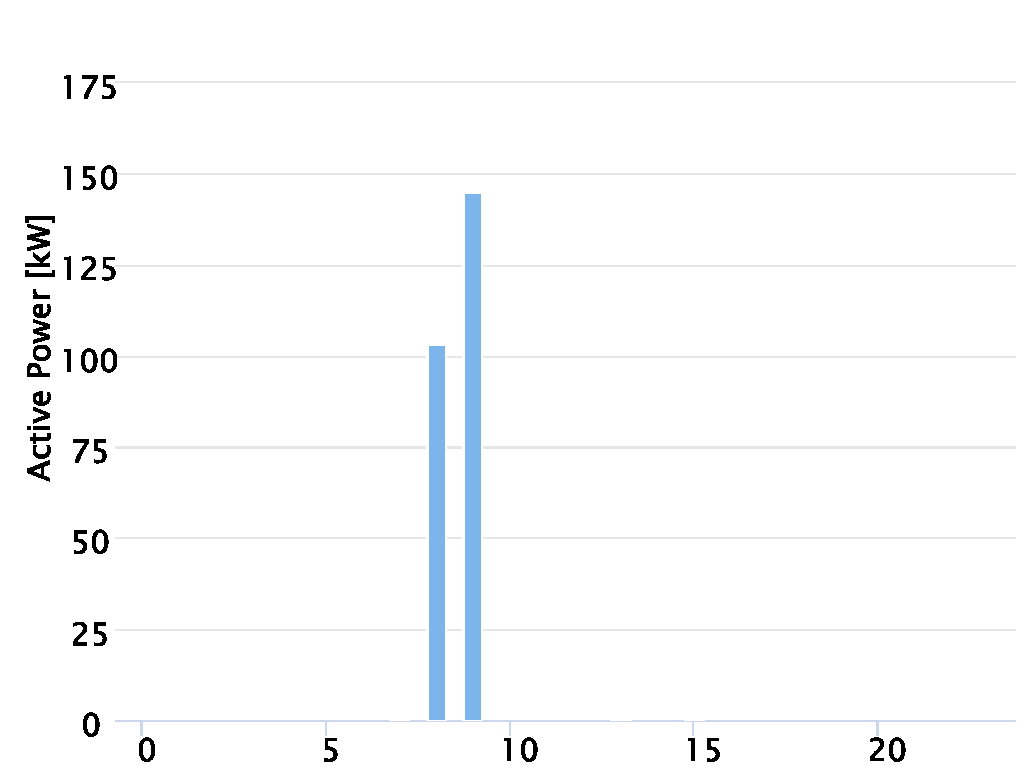
\includegraphics[width=0.45\textwidth]{Figures/2_case/pv-curtailment.pdf}
        \label{fig:case_II_pv_curt_dispatch}
    }
    \subfloat[Case IV: Contingency at 08:00 h with \glspl{ev}.]{
        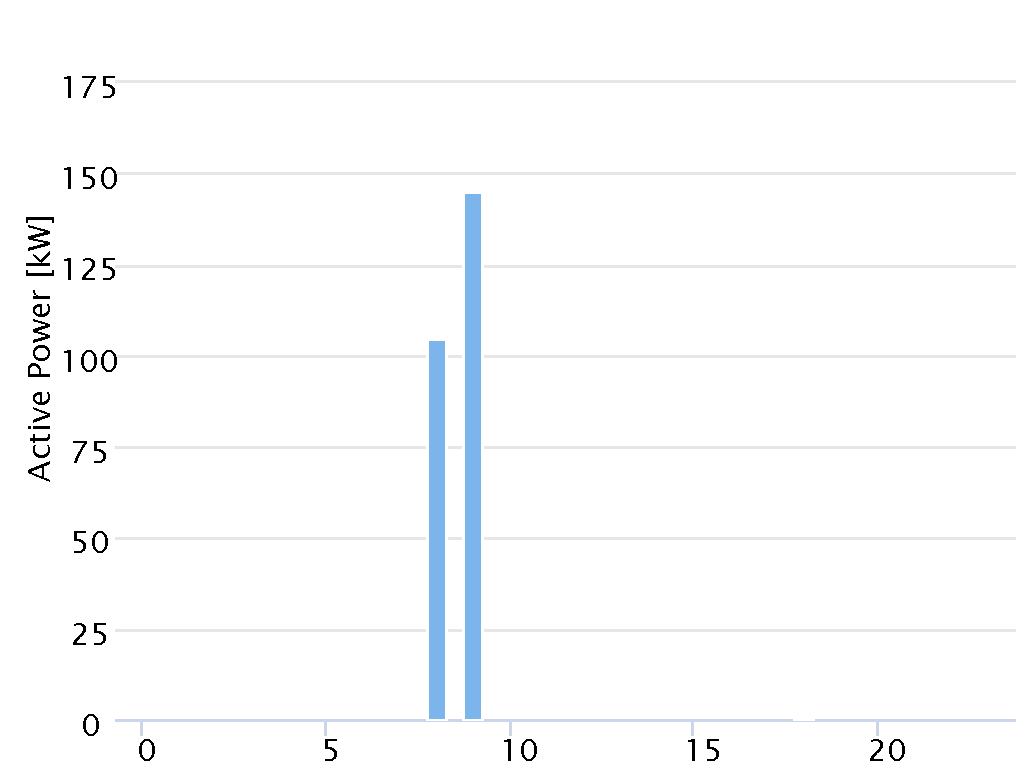
\includegraphics[width=0.45\textwidth]{Figures/4_case/pv-curtailment.pdf}
        \label{fig:case_IV_pv_curt_dispatch}
    }
    \vfill
    \subfloat[Case V: Contingency at 16:00 h with \glspl{ev}.]{
        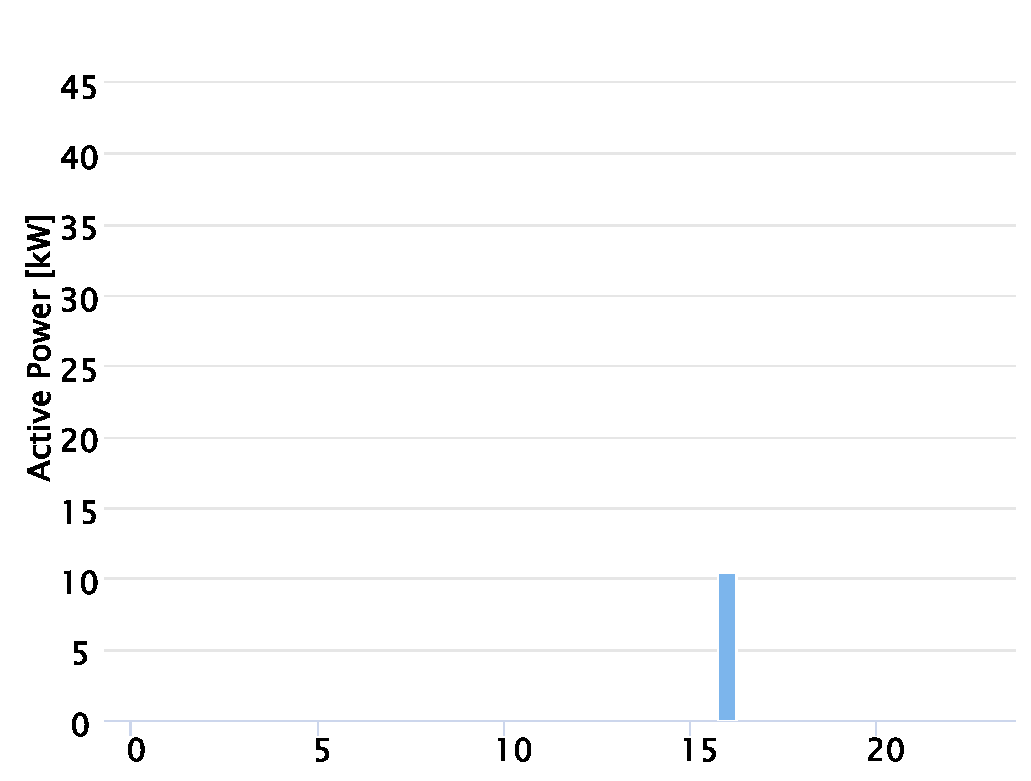
\includegraphics[width=0.45\textwidth]{Figures/5_case/pv-curtailment.pdf}
        \label{fig:case_V_pv_curt_dispatch}
    }
    \subfloat[Case VI: Contingencies at 08:00 and 16:00 hours with \glspl{ev}.]{
        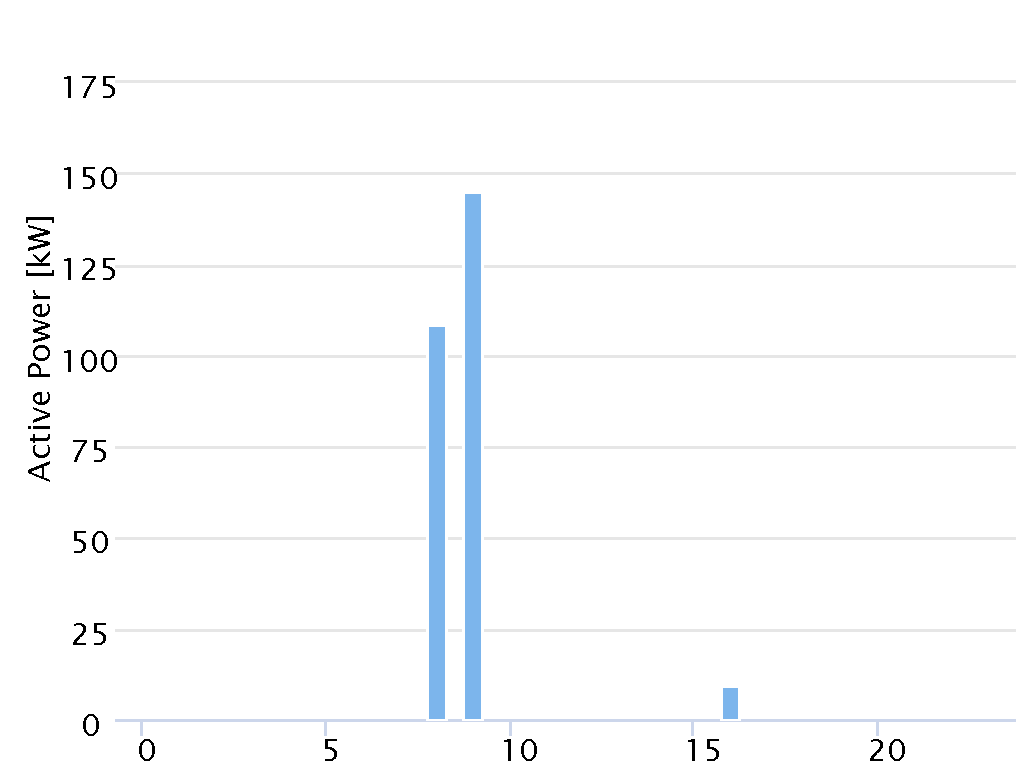
\includegraphics[width=0.45\textwidth]{Figures/6_case/pv-curtailment.pdf}
        \label{fig:case_VI_pv_curt_dispatch}
    }
    \caption{PV reduction for each case.}
    \label{fig:pv_curtailment_dispatch}
\end{figure*}

\begin{figure*}[!h]
    \centering
    \subfloat[Case III: Without contingencies, including \glspl{ev}.]{
        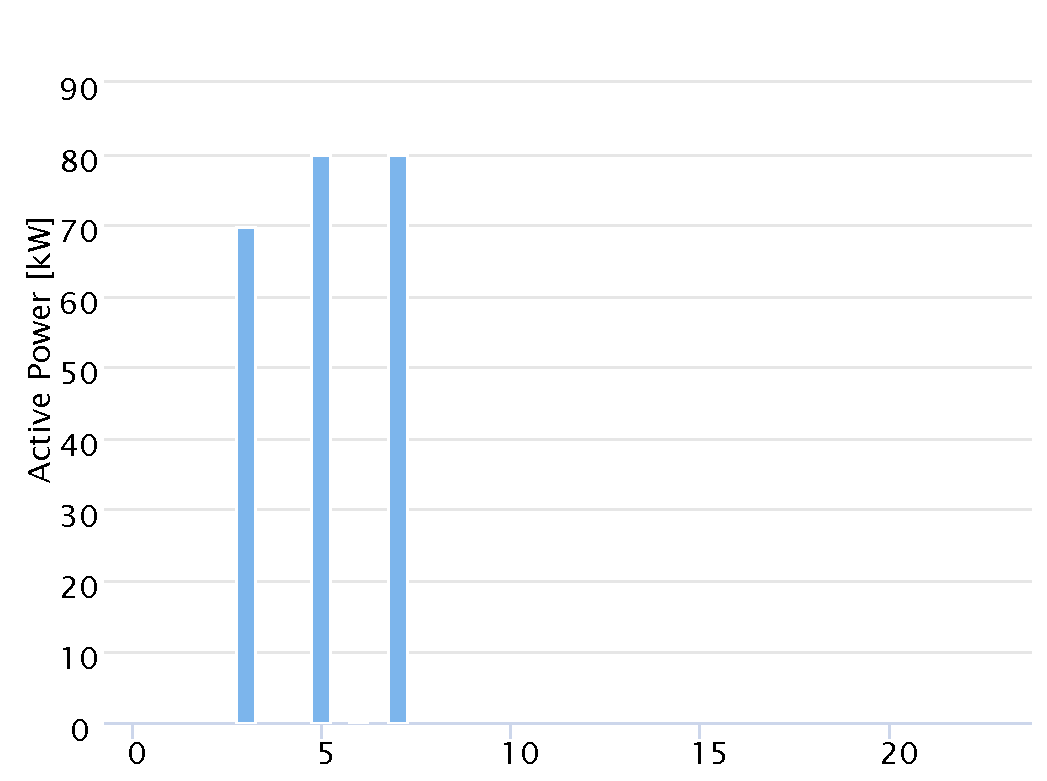
\includegraphics[width=0.45\textwidth]{Figures/3_case/ev_1.pdf}
        \label{fig:case_III_ev1_dispatch}
    }
    \subfloat[Case IV: Contingency at 08:00 h with \glspl{ev}.]{
        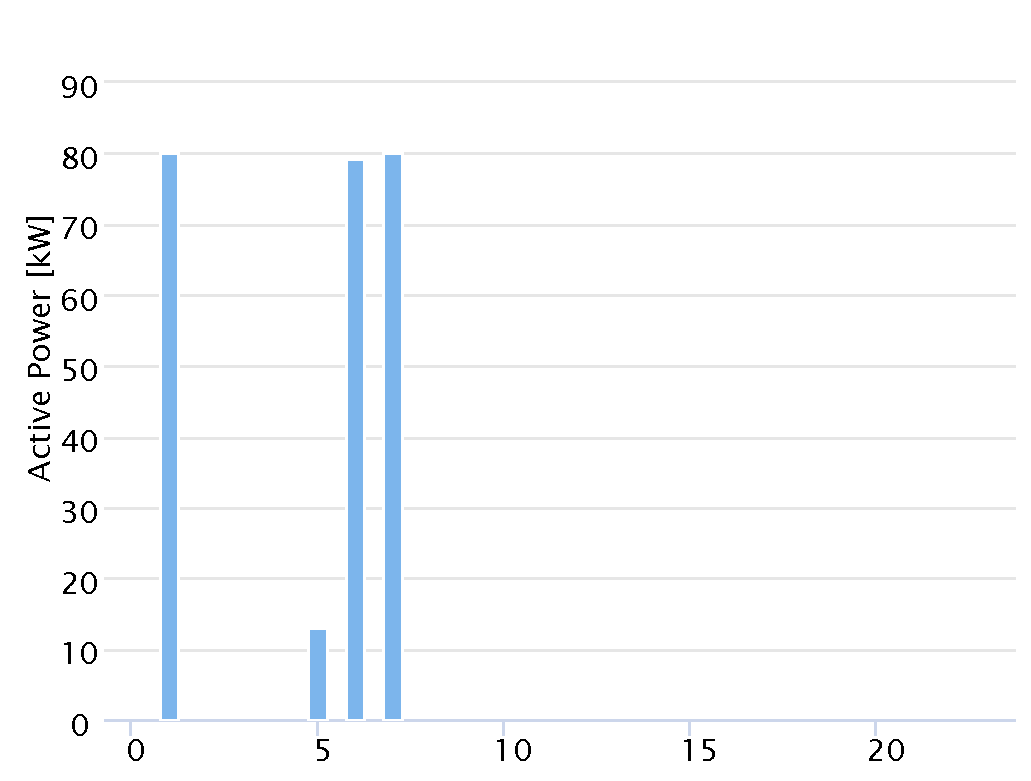
\includegraphics[width=0.45\textwidth]{Figures/4_case/ev_1.pdf}
        \label{fig:case_IV_ev1_dispatch}
    }
    \vfill
   \subfloat[Case V: Contingency at 16:00 h with \glspl{ev}.]{
        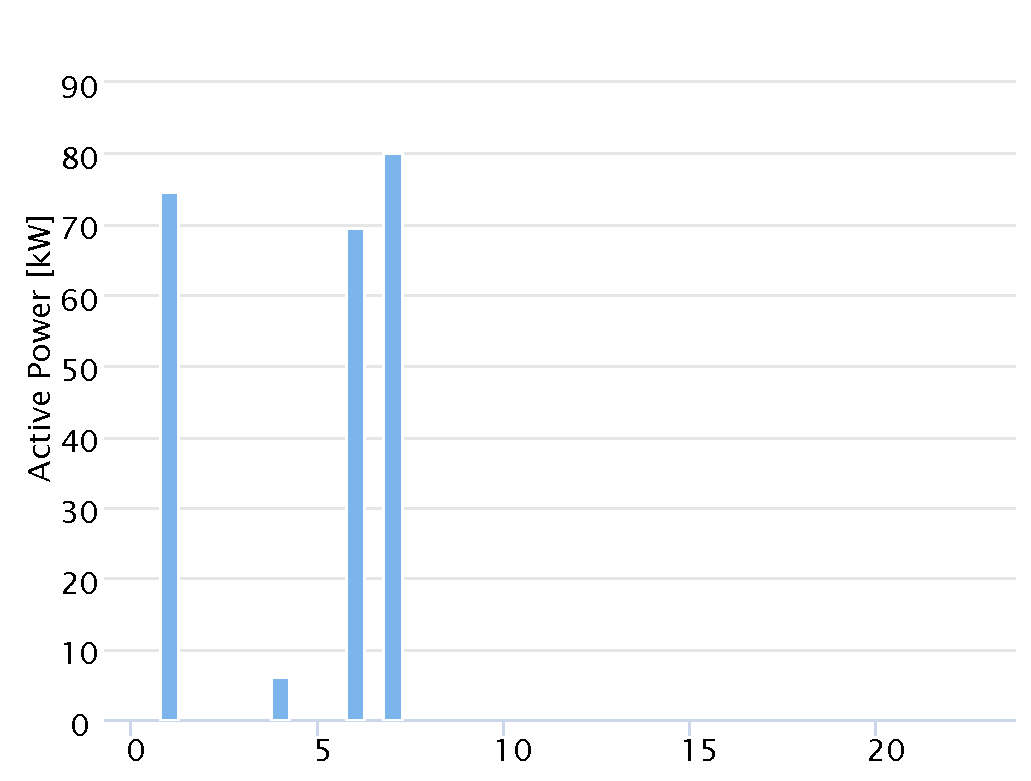
\includegraphics[width=0.45\textwidth]{Figures/5_case/ev_1.pdf}
        \label{fig:case_V_ev1_dispatch}
    }
    \subfloat[Case VI: Contingencies at 08:00 and 16:00 hours with \glspl{ev}.]{
        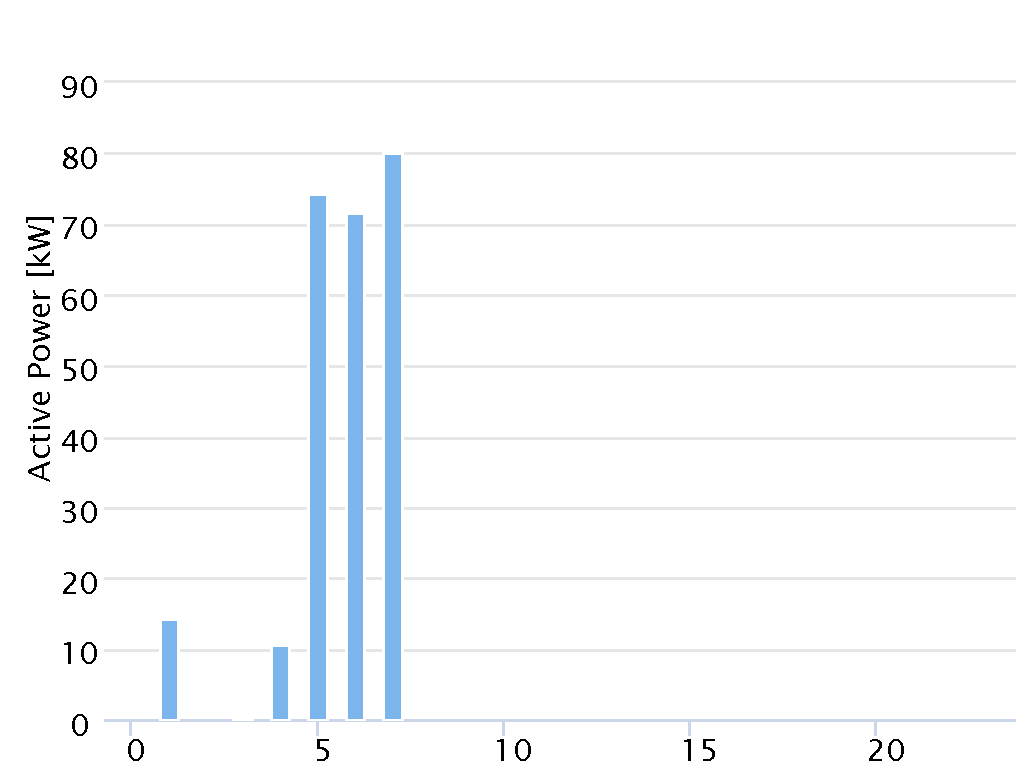
\includegraphics[width=0.45\textwidth]{Figures/6_case/ev_1.pdf}
        \label{fig:case_VI_ev1_dispatch}
    }
    \caption{E-Bus dispatch for each case.}
    \label{fig:ev_1_2_dispatch}
\end{figure*}

\begin{figure}[!h]
    \centering
    \subfloat[Case III: Without contingencies, including \glspl{ev}.]{
        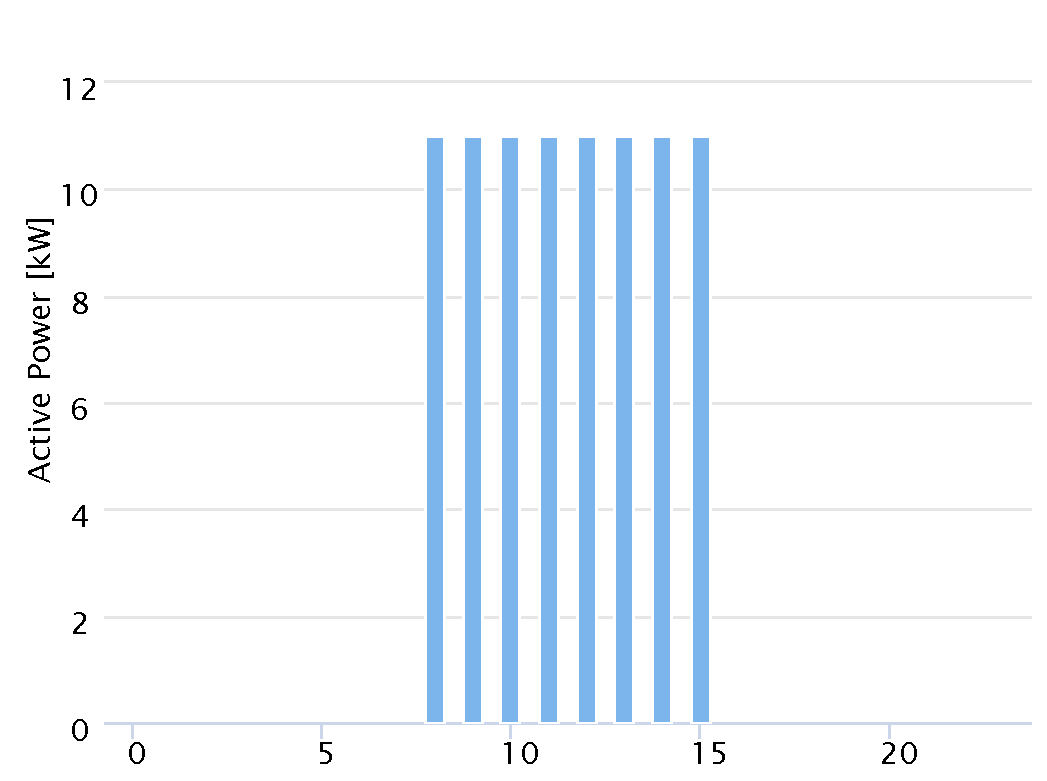
\includegraphics[width=0.45\textwidth]{Figures/3_case/ev_2.pdf}
        \label{fig:case_III_ev2_dispatch}
    }
    \subfloat[Case IV: Contingency at 08:00 h with \glspl{ev}.]{
        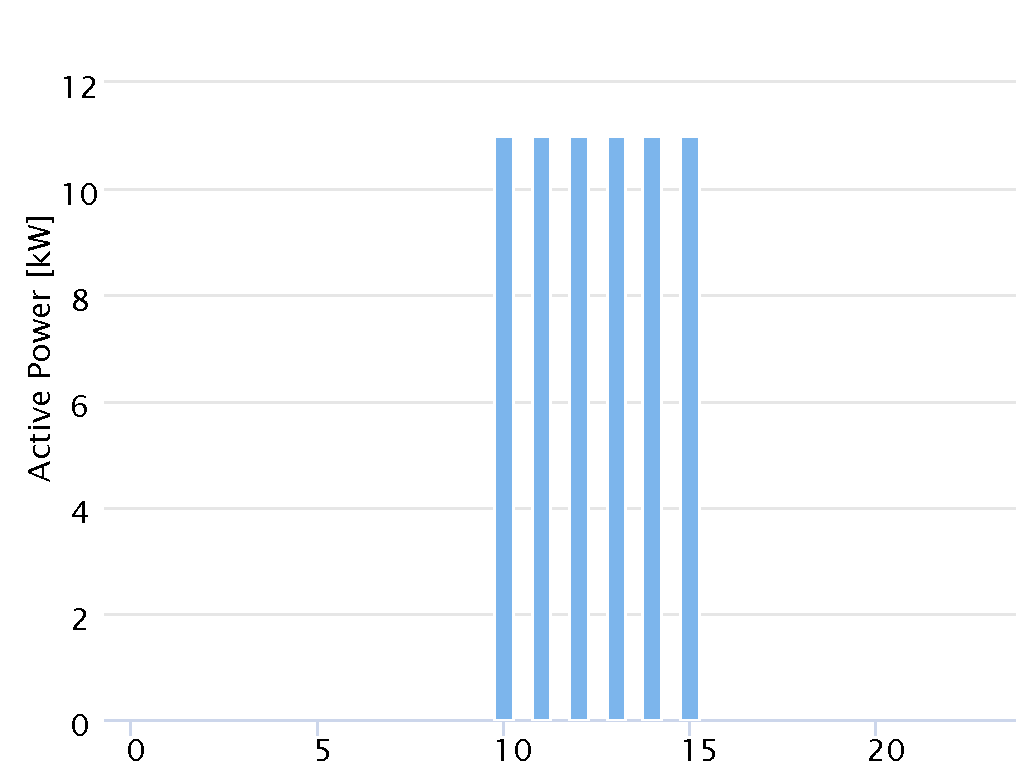
\includegraphics[width=0.45\textwidth]{Figures/4_case/ev_2.pdf}
        \label{fig:case_IV_ev2_dispatch}
    }
    \vfill
   \subfloat[Case V: Contingency at 16:00 h with \glspl{ev}.]{
        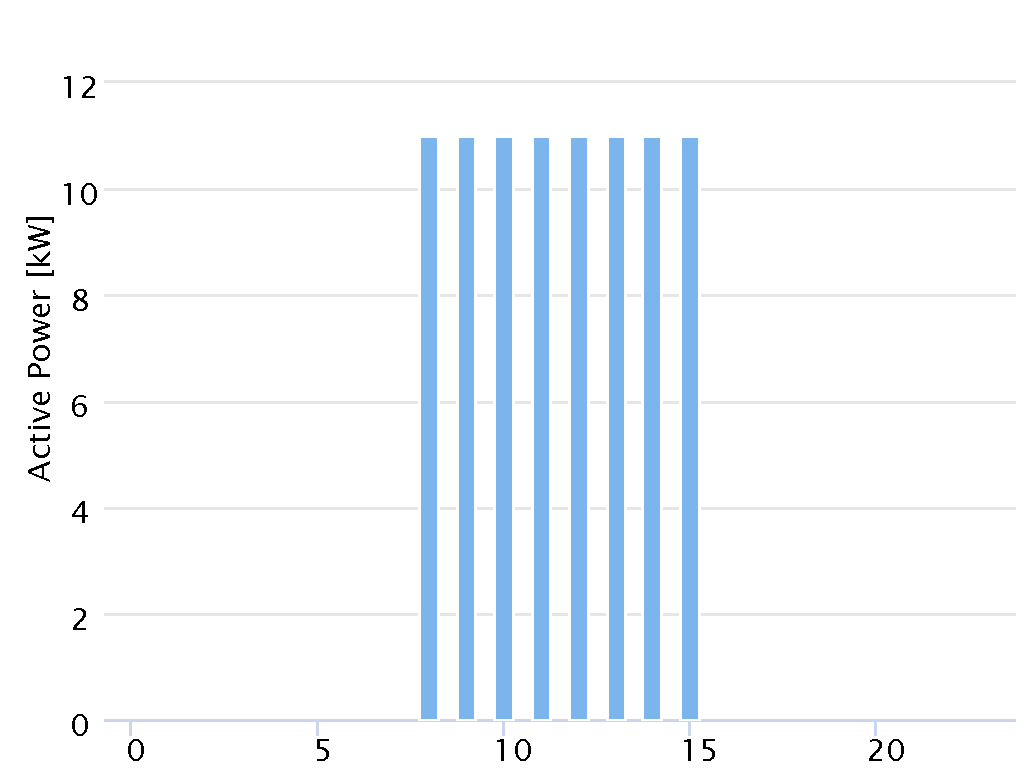
\includegraphics[width=0.45\textwidth]{Figures/5_case/ev_2.pdf}
        \label{fig:case_V_ev2_dispatch}
    }
    \subfloat[Case VI: Contingencies at 08:00 and 16:00 hours with \glspl{ev}.]{
        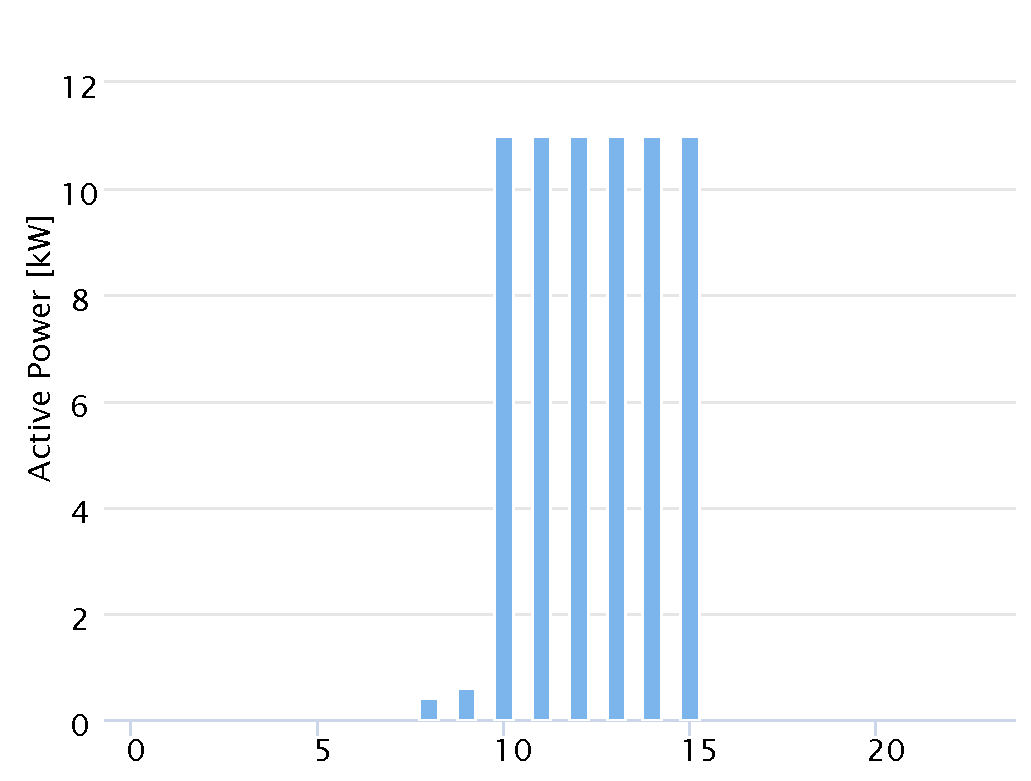
\includegraphics[width=0.45\textwidth]{Figures/6_case/ev_2.pdf}
        \label{fig:case_VI_ev2_dispatch}
    }
    \caption{EV dispatch for each case.}
    \label{fig:ev_2_dispatch}
\end{figure}

\begin{figure*}[!h]
    \centering
    \subfloat[Case V: Contingency at 16:00 h with \glspl{ev}.]{
        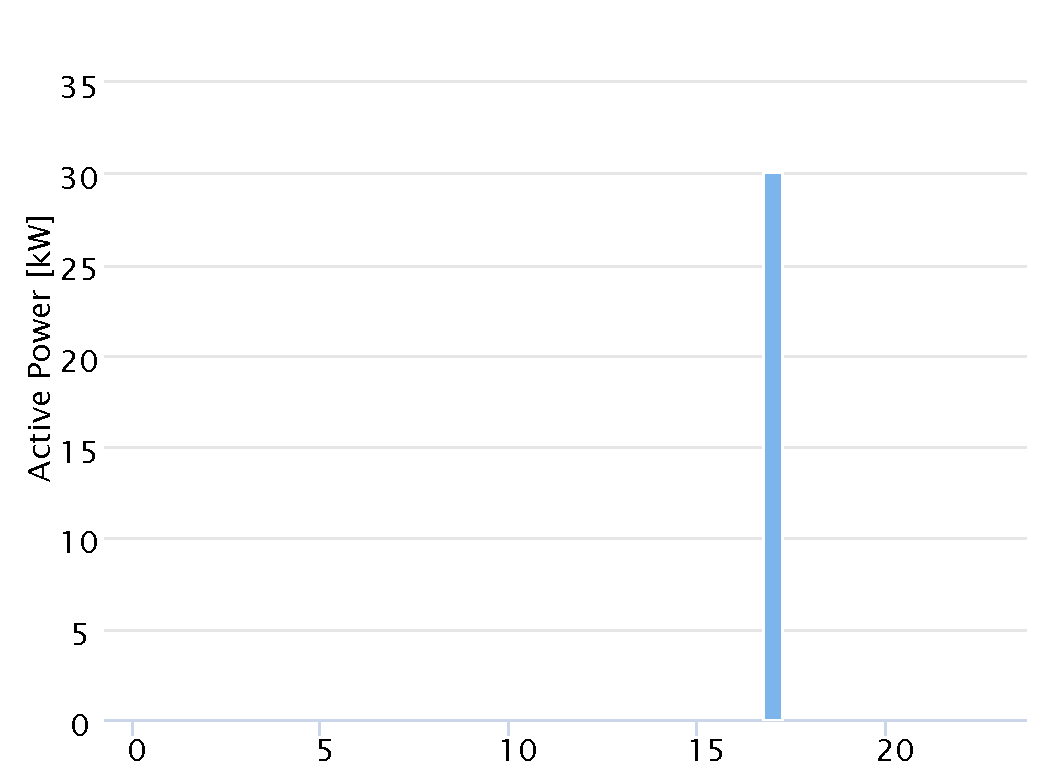
\includegraphics[width=0.45\textwidth]{Figures/5_case/genset-dispatch.pdf}
        \label{fig:case_V_genset_dispatch}
    }
    \subfloat[Case VI: Contingencies at 08:00 and 16:00 hours with \glspl{ev}.]{
        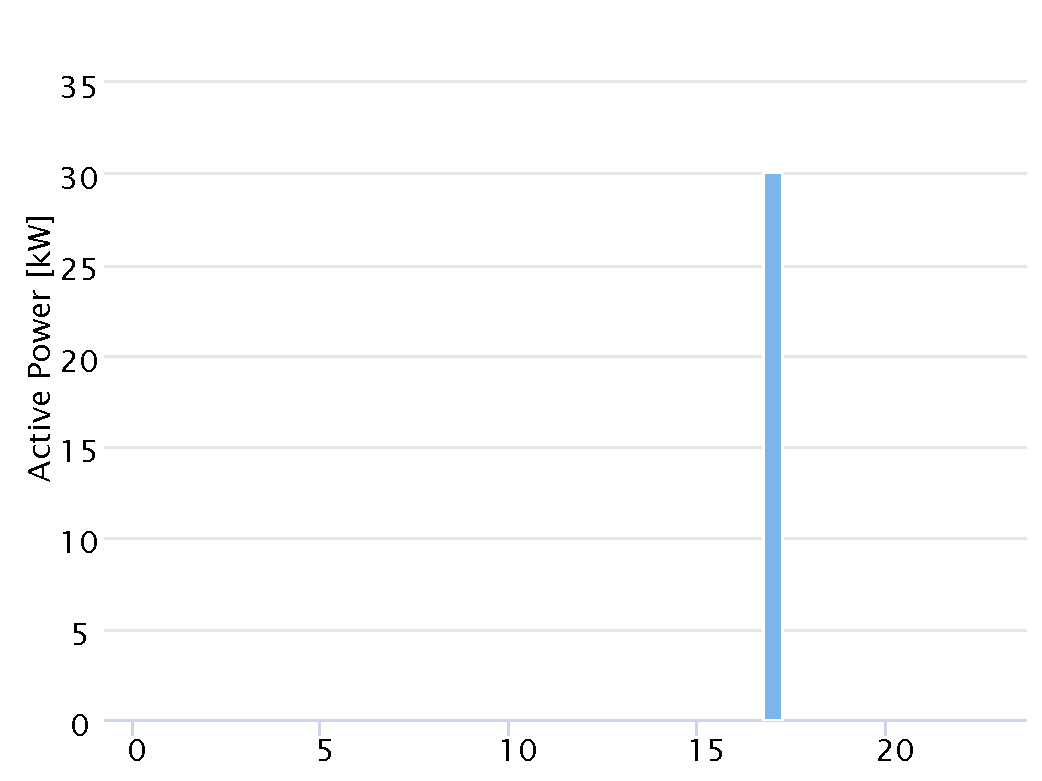
\includegraphics[width=0.45\textwidth]{Figures/6_case/genset-dispatch.pdf}
        \label{fig:case_VI_genset_dispatch}
    }
    \caption{Genset dispatch for each case.}
    \label{fig:genset_genset_dispatch}
\end{figure*}




\begin{figure}[!ht]
    \centering
    
\includegraphics[width=0.5\textwidth]{Figures/2_case/legenda.pdf}
    \vfill
    \subfloat[Case I: Without contingencies.]{
        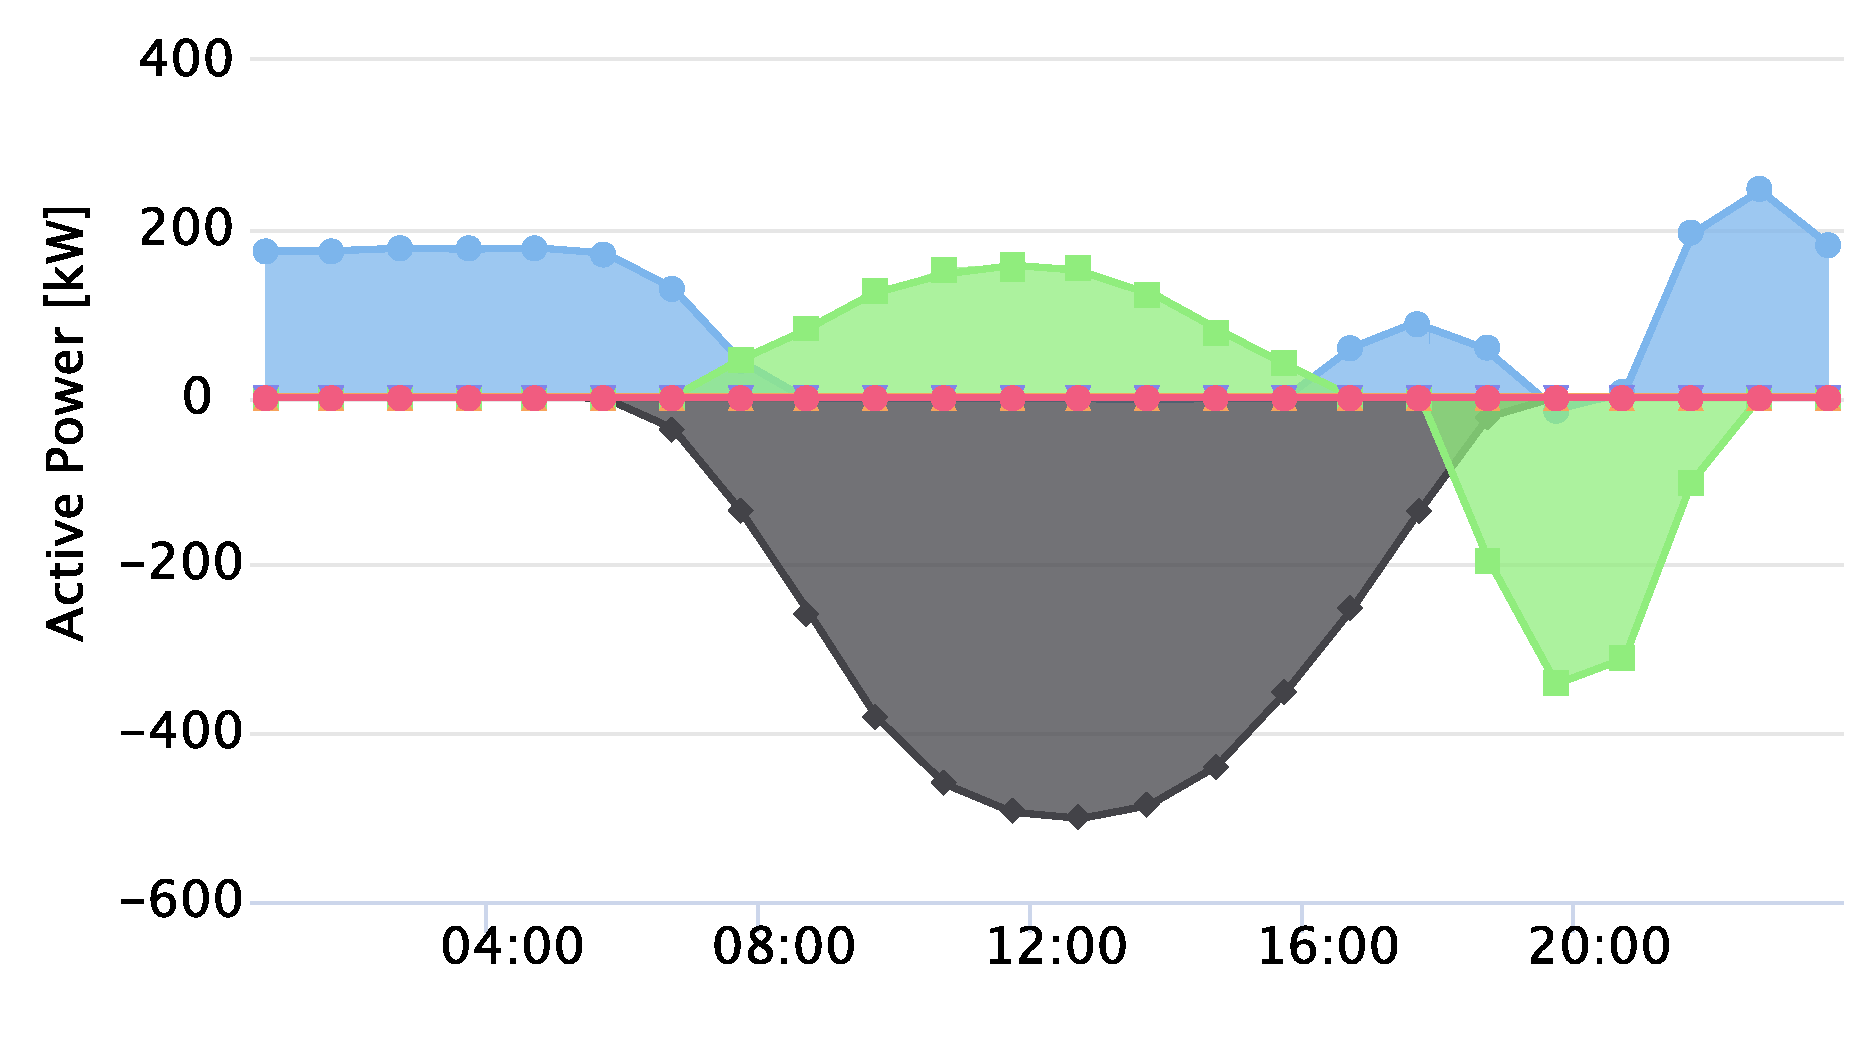
\includegraphics[width=0.45\textwidth]{Figures/1_case/microgrid-operation.pdf}
        \label{fig:case_I_operation}
    }
    \subfloat[Case II: Contingency at 08:00 h.]{
        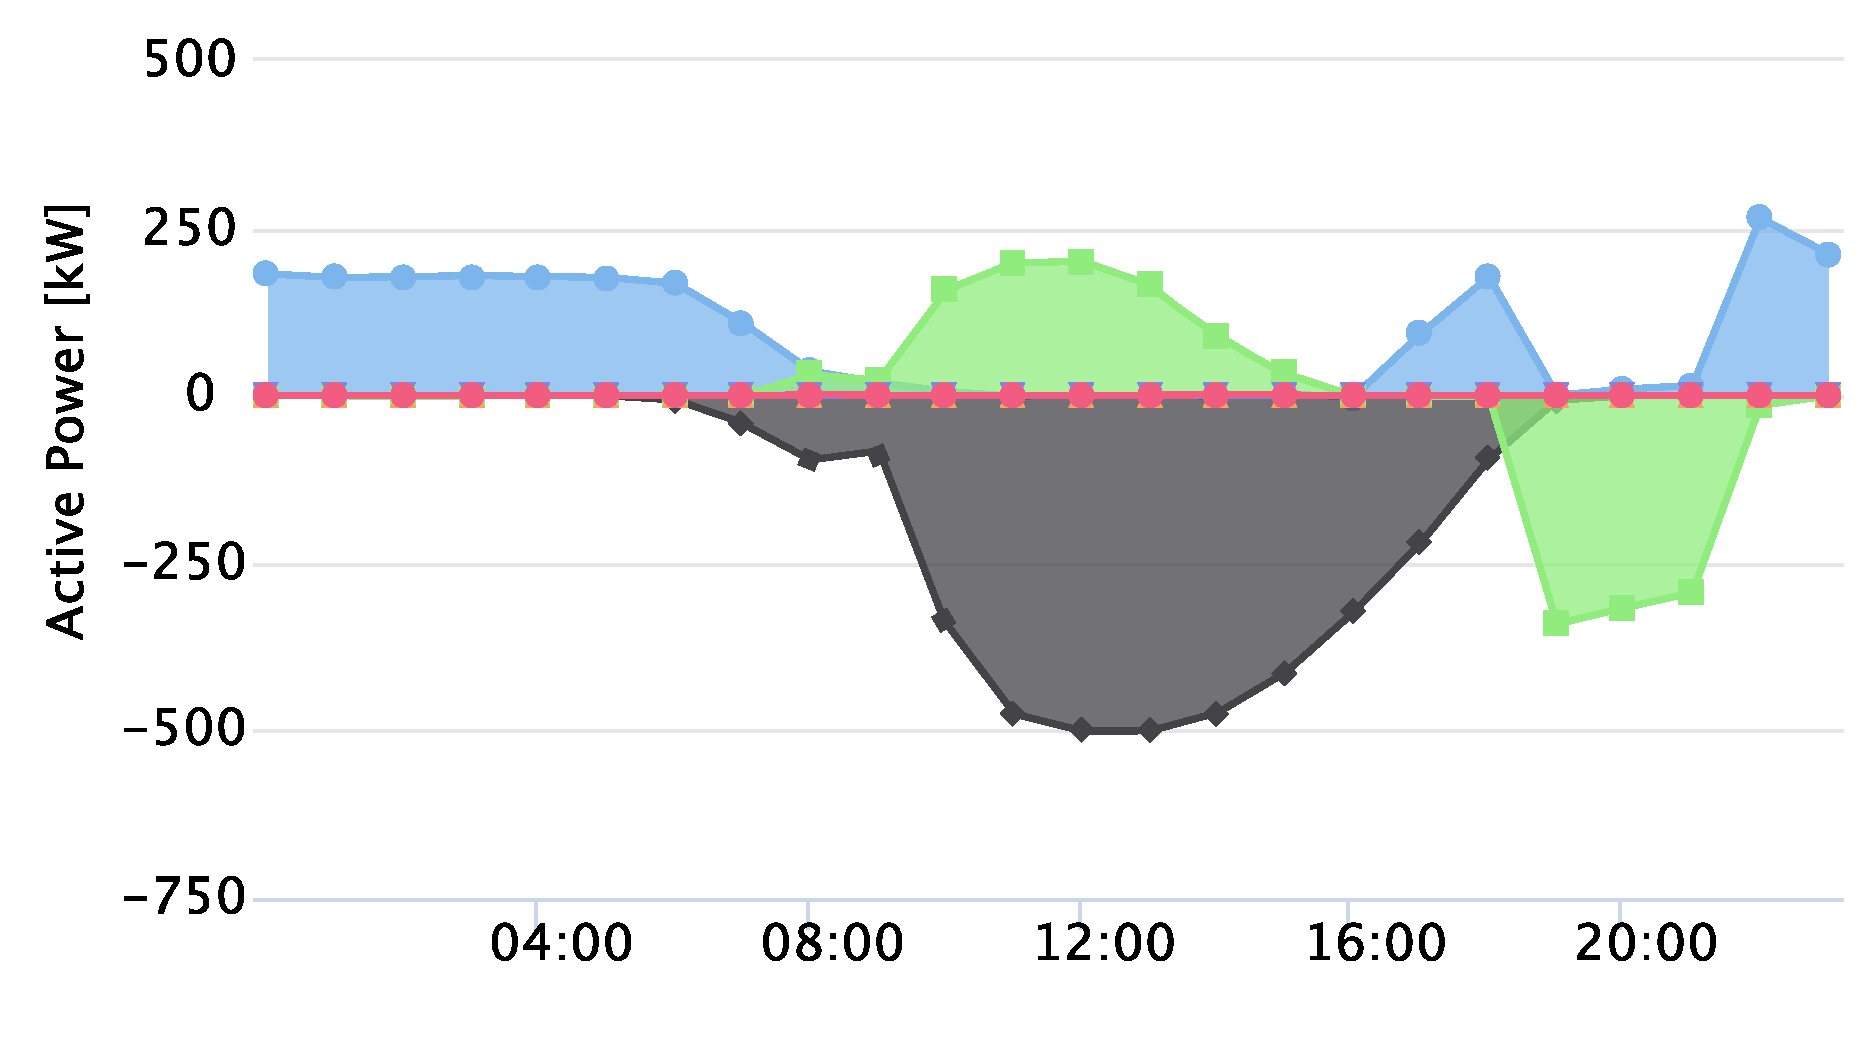
\includegraphics[width=0.45\textwidth]{Figures/2_case/microgrid-operation.pdf}
        \label{fig:case_II_operation}
    }
    \vfill
    \subfloat[Case III: Without contingencies, including \glspl{ev}.]{
        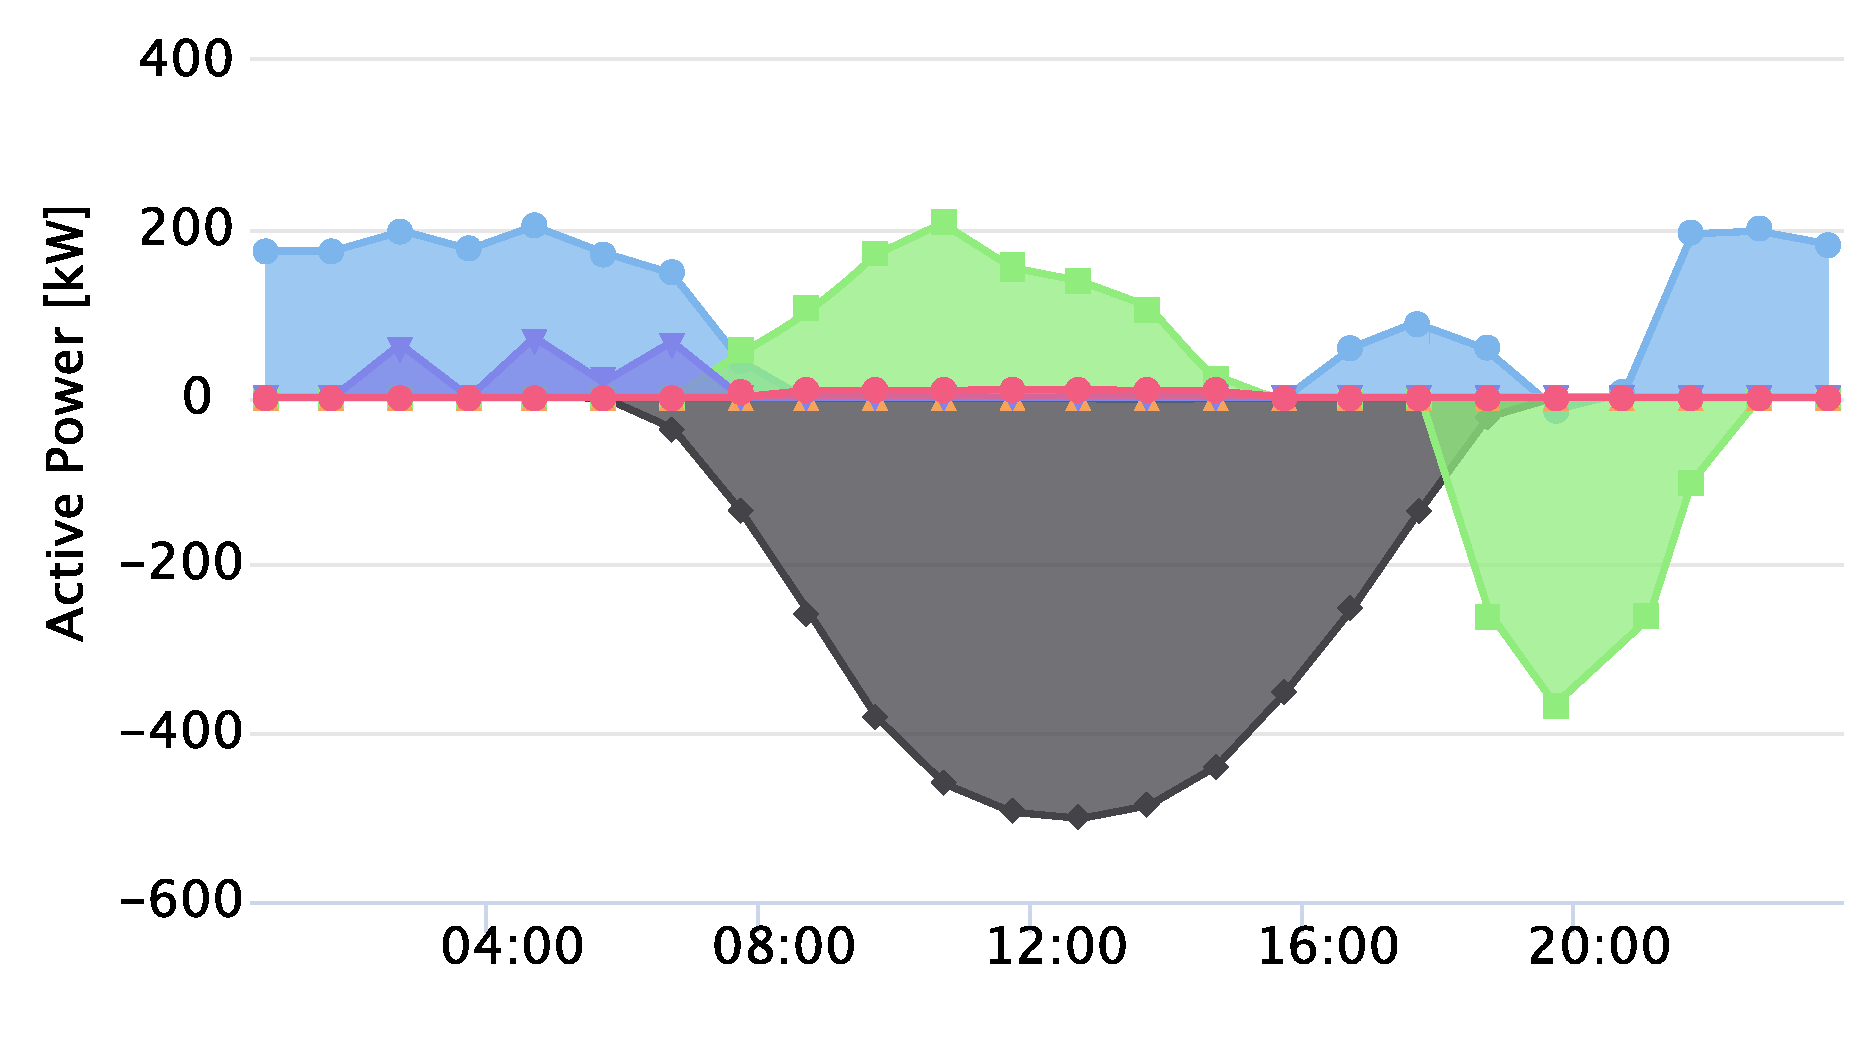
\includegraphics[width=0.45\textwidth]{Figures/3_case/microgrid-operation.pdf}
        \label{fig:case_III_operation}
    }
    \subfloat[Case IV: Contingencies at 08:00 and 16:00 hours with \glspl{ev}.]{
        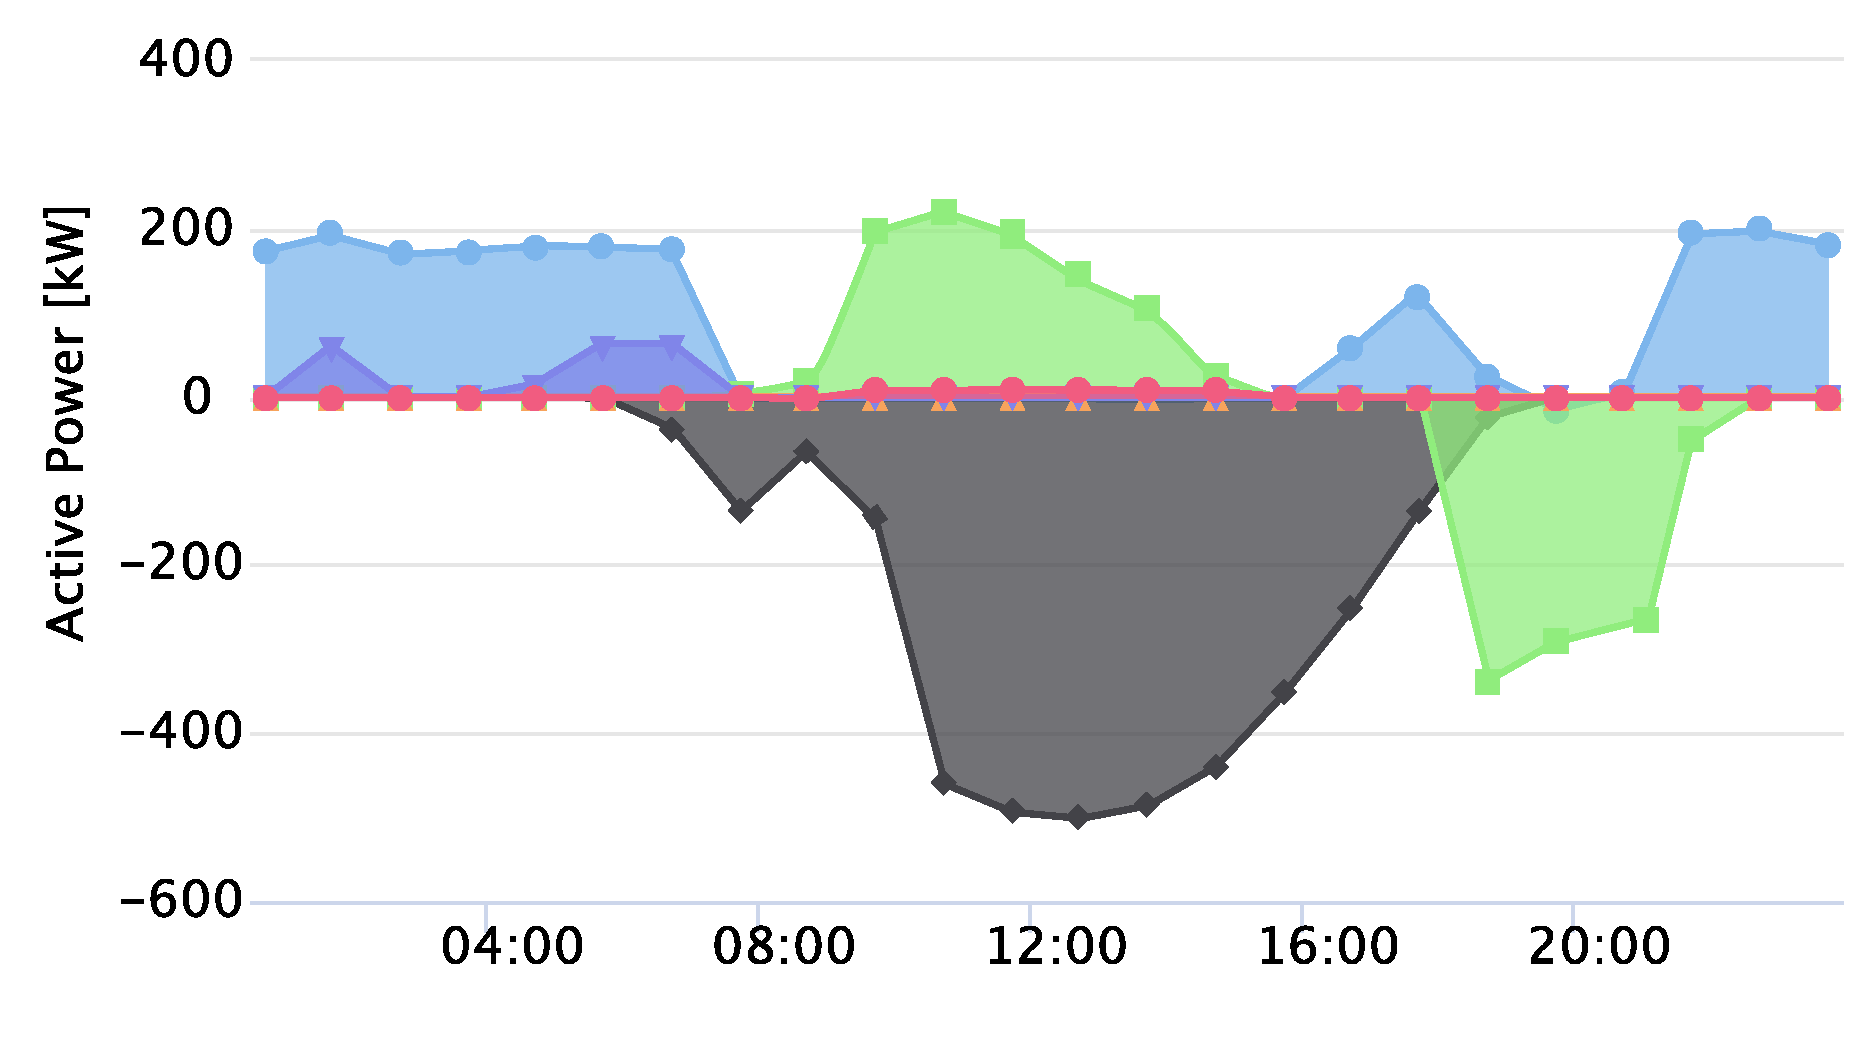
\includegraphics[width=0.45\textwidth]{Figures/4_case/microgrid-operation.pdf}
        \label{fig:case_IV_operation}
    }
    \vfill
    \subfloat[Case V: Contingency at 16:00 h with \glspl{ev}.]{
        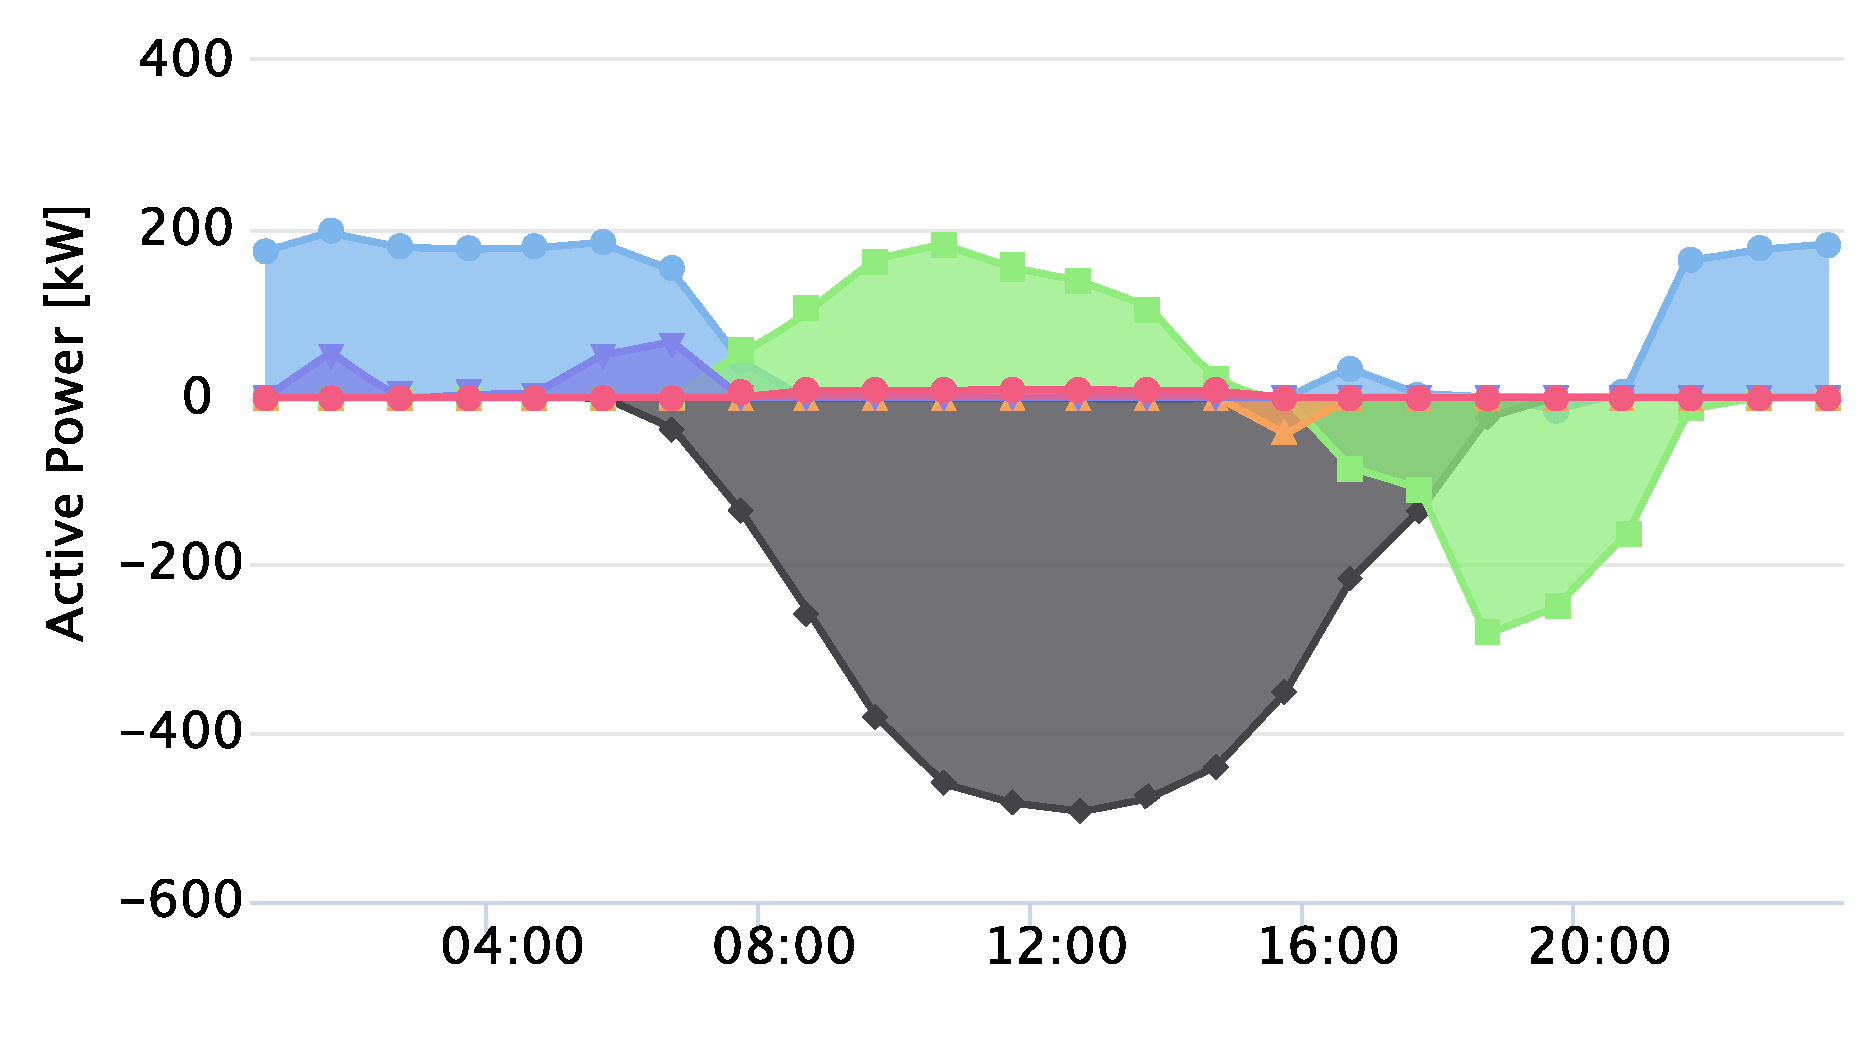
\includegraphics[width=0.45\textwidth]{Figures/5_case/microgrid-operation.pdf}
        \label{fig:case_V_operation}
    }
    \subfloat[Case VI: Contingencies at 08:00 and 16:00 hours with \glspl{ev}.]{
        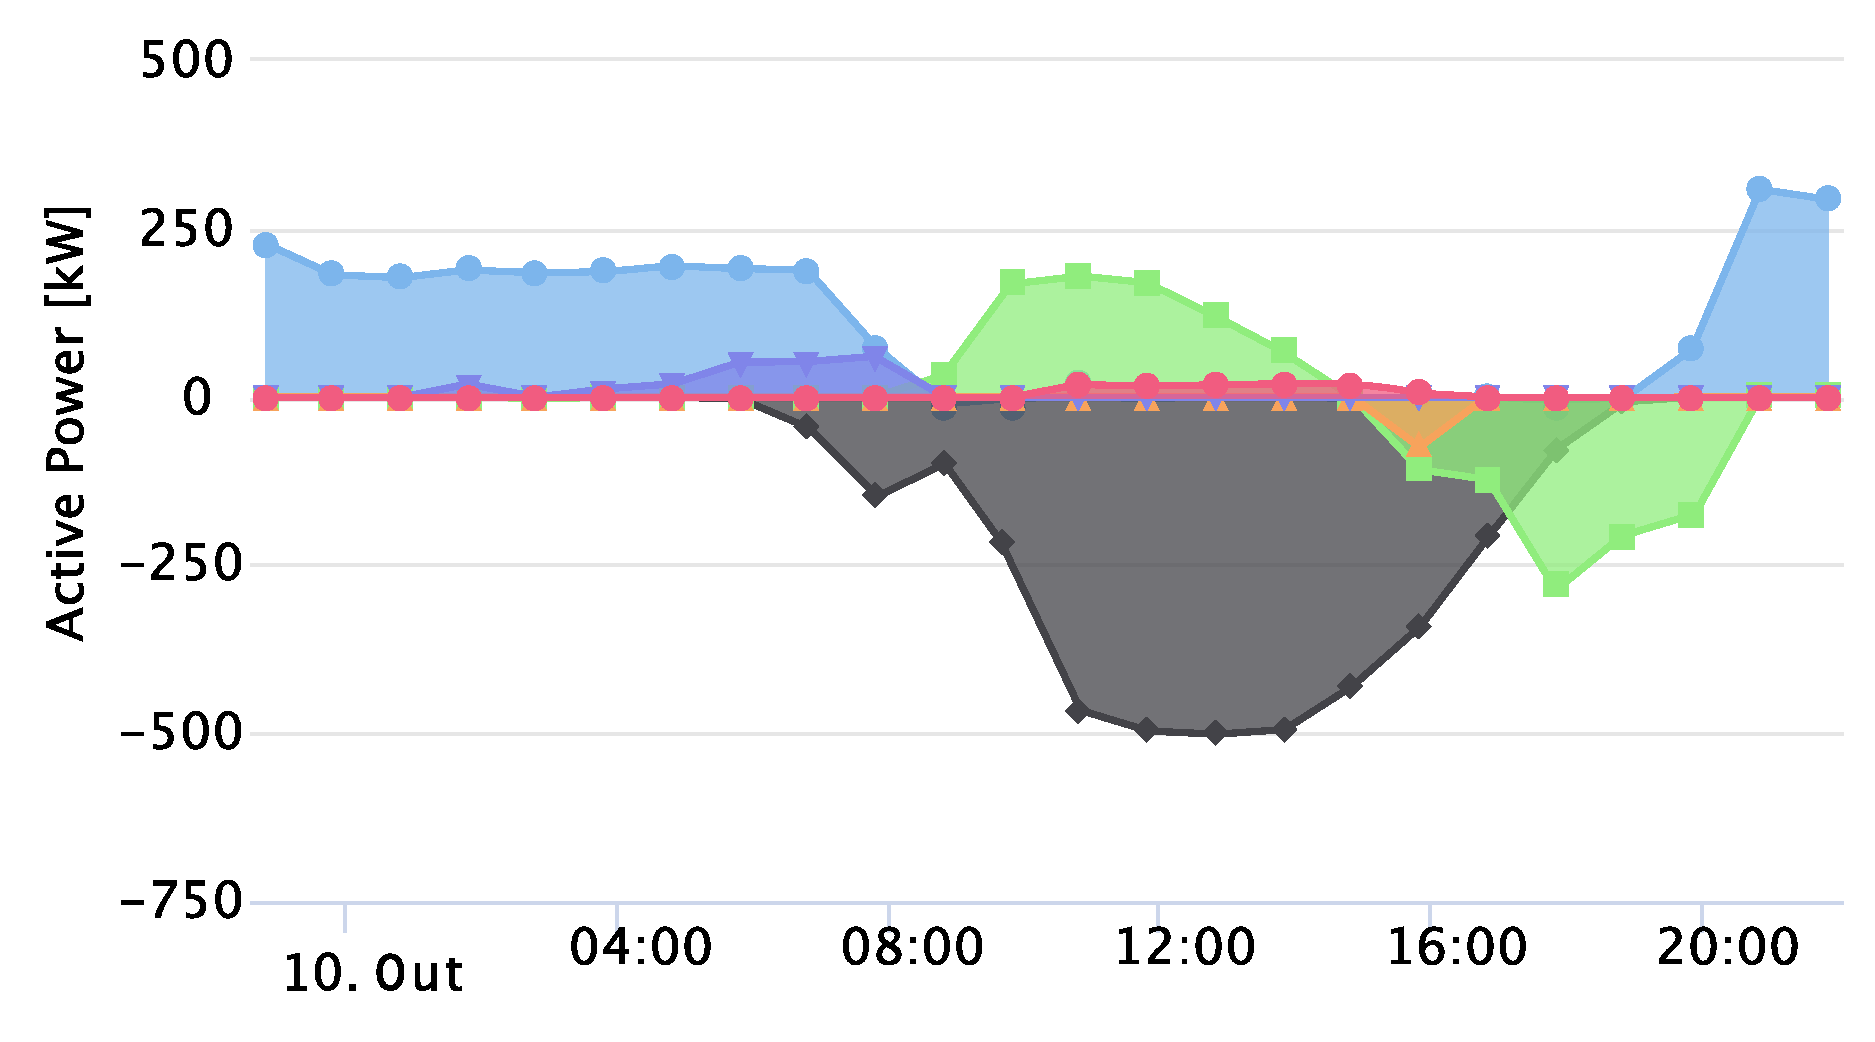
\includegraphics[width=0.45\textwidth]{Figures/6_case/microgrid-operation.pdf}
        \label{fig:case_VI_operation}
    }
    \caption{Microgrid 24 h for each case study.}
    \label{fig:microgrid_operation}
\end{figure}

Case I represents the normal operation of the microgrid 
without any contingencies. The optimal dispatch of the \gls{bess} takes 
advantage of the PV generation to charge during the high \gls{pv} and 
discharge during the high energy cost periods, according to the energy prices outlined in \ref{sec:case_study}.
Fig. \ref{fig:case_I_bess_dispatch} shows the BESS dispatch, while
Fig. \ref{fig:case_I_operation} illustrates the microgrid's 24-hours 
operation. 

In Case II, the \gls{bess} begins to charge significantly at  10:00\,h, although a very small amount of charging is observed before and
during the contingency (see Fig. \ref{fig:case_II_bess_dispatch}). It discharges during peak energy periods at night. 
Additionally,  Fig. \ref{fig:case_II_pv_curt_dispatch} shows a \gls{pv} 
reduction during the two contingency hours, this occurs because, during the contingency, exporting energy to the grid is 
not possible. Furthermore, as the model aims to minimize energy imported from the grid, it prioritizes supplying the entire demand of the 
microgrid. Once the demand is met, any excess generation from the 
\gls{pv} must be reduced using the \gls{pv} reduction mechanism 
enabled by the inverters. These measurements are shown in the 
microgrid's operation in Fig.\ref{fig:case_II_operation}.

Unlike the first and second cases, Case III includes the microgrid operation with \glspl{ev}. The \gls{bess} dispatch is similar to the first case, charging during high \gls{pv} generation and discharging at night during peak energy periods, as can be seen in the Fig.~\ref{fig:case_III_bess_dispatch}. Regarding the charging and fairness for the \glspl{ev}, the E-bus has a higher capacity (324\,kWh), the same \gls{soc} level (20\% for both), but less available charging time (7 h vs. 9 h). Here, the \gls{ev} receives a slightly higher weight (0.52) compared to the E-bus (0.48). The E-bus gets 264.3\,kWh, while the \gls{ev} receives all its required energy (108\,kWh). This results in a balanced energy distribution, with a slight preference for the \gls{ev} due to its longer charging window. The dispatch for both \glspl{ev} are shown in Figs. \ref{fig:case_III_ev1_dispatch} and \ref{fig:case_III_ev2_dispatch}. Additionally, EV and E-bus charging and microgrid operation can be seen in Fig.~\ref{fig:case_III_operation}.

Case IV shows the \gls{bess} dispatch similar to Case II, but with \gls{pv} reduction occurring only during the two contingency hours (08:00 to 09:00 hours), see Fig. \ref{fig:case_IV_bess_dispatch} and Fig. \ref{fig:case_IV_pv_curt_dispatch}. Regarding \glspl{ev} charging, due to the contingency during the first two hours, charging only occurs after this period, reducing the charging time to 7 hours. Thus, the fairness analysis mirrors Case II in Table \ref{tab:fairness_analysis}, with the same \gls{soc} level, 7 hours of charging time, but different energy capacities. As a result, the E-bus receives a higher priority due to its greater energy needs. The E-bus is fully charged (324 kWh), while the \gls{ev} charges only 84.3 kWh. The \glspl{ev} dispatches are illustrated in Figs.
\ref{fig:case_IV_ev1_dispatch} and \ref{fig:case_IV_ev2_dispatch}, and the operation are shown in Fig.~\ref{fig:case_IV_operation}.

For Case V, the \gls{bess} charges similar to the previous cases but begins discharging during the two contingency hours (16:00 to 17:00) to support the microgrid's demand, along with the \gls{genset} dispatch (see Figs. \ref{fig:case_V_bess_dispatch} and \ref{fig:case_V_genset_dispatch}). Additionally, small reduction in \gls{pv} generation are observed during the first contingency hour (see Fig. \ref{fig:case_V_pv_curt_dispatch}). In terms of \glspl{ev} fairness, the same weight and energy distribution from Case III is repeated (see Figs. \ref{fig:case_V_ev1_dispatch} and \ref{fig:case_V_ev2_dispatch}). All these dispatches are reflected in the overall microgrid operation shown in Fig. \ref{fig:case_V_operation}.

Finally, Case VI involves two contingencies. The \gls{bess} begins to charge significantly at 
10:00 hours, with a very small amount of charge during the second hour of the first contingency and discharges during the second contingency (16:00 to 17:00 h) to support the microgrid along with the \gls{genset} (see Figs. \ref{fig:case_VI_bess_dispatch} and \ref{fig:case_VI_genset_dispatch}). \gls{pv} reduction occurs only during the first contingency (08:00 to 09:00 h) (see Fig. \ref{fig:case_VI_pv_curt_dispatch}). In terms of \glspl{ev} fairness, the same weight and energy distribution from Case IV is applied (see Figs. \ref{fig:case_VI_ev1_dispatch} and \ref{fig:case_VI_ev2_dispatch}). All these analyses are reflected in the microgrid operation, shown in Fig. \ref{fig:case_VI_operation}.


In summary, the results highlight the microgrid’s adaptability across diverse scenarios, including contingencies and \gls{ev} integration. Case I demonstrated optimal, cost-efficient operation without contingencies. In Cases II to VI, the system effectively prioritized loads during contingencies, managed \gls{pv} reduction, and balanced energy distribution between \glspl{ev} and the E-bus. Case VI, with dual contingencies, showcased the system’s robustness, leveraging the BESS and \gls{genset} for stable operation. Overall, the microgrid efficiently met demand and maintained fairness in \gls{ev} charging, proving capable of handling disruptions and varying energy needs.

\glsresetall

\section{Conclusions}\label{sec:conclusions}

The multi-objective optimization approach developed in this work successfully addressed the energy management of a microgrid with \glspl{ev}. The algorithm presented in \ref{subsec:moop} yielded a set of non-dominated solutions forming the Pareto front, which provided crucial insights into the trade-offs between \gls{ens} for \glspl{ev} ($f_{ens}$) and operational costs for the microgrid ($f_{costs}$). 

From the Pareto front analysis, two extreme points were identified. The first extreme point achieved a maximum environmental performance ($\varepsilon_{p} = 345.6$ kWh) at the lowest cost ($17,645$), prioritizing cost minimization over energy provision for \glspl{ev}. Conversely, the second extreme point reflected the highest cost ($20,313$) associated with full charging of the \glspl{ev}, demonstrating a commitment to environmental sustainability despite increased operational expenses.

The fairness index effectively prioritizes \glspl{ev} with higher energy demands or longer charging times, but all vehicles are allocated energy proportional to their needs and time constraints. Various case studies demonstrated that the system allocated energy in a way that prioritized vehicles with greater needs or more available charging time. In Case I, even with equal demand, disparities in energy distribution emerged due to the adoption of the selected $\varepsilon_{p}$ value. Subsequent cases further reinforced this trend, showing that weights assigned to each vehicle based on their energy requirements played a pivotal role in ensuring equitable energy allocation.

The analysis of the six cases showed the operation of the microgrid under various conditions. Case I demonstrates optimal performance without contingencies, i.e., only grid-connected operation, effectively utilizing \gls{bess} and \gls{pv} resources to supply demand and reduce costs. Other cases highlight the impact of contingencies and the integration of \glspl{ev}, showcasing the fairness analysis for the E-bus and \gls{ev}. Furthermore, Case VI demonstrates the adaptability of the microgrid in the face of a more critical scenario, with the \gls{bess} supporting demand during contingencies while managing \gls{pv} reduction. 

Overall, the results underscore the potential of the proposed approach to optimize energy distribution in microgrids, ensuring fairness among EVs while enhancing both objectives.

\appendix

\section{Piecewise Linearization}\label{appndx:piecewise}

The quadratic terms $(P_{ij,f,ht,c})^2$, 
$(Q_{ij,h,t,c})^2$, $(P_{i,f,t,c}^{\text{PCC}})^2$ and  
$(Q_{i,f,t,c}^{\text{PCC}})^2$ in (\ref{I}) and 
(\ref{pcc}) are linearized using a linear piecewise approximation function as 
presented in \cite{silva2021}. To linearize the terms 
$(P_{ij,f,ht,c})^2$, $(Q_{ij,h,t,c})^2$, $(P_{i,f,t,c}^{\text{PCC}})^2$ and 
$(Q_{i,f,t,c}^{\text{PCC}})^2$, the variables 
$(P_{ij,f,ht,c}^{sqr})^2$, $(Q_{ij,h,t,c}^{sqr})^2$, 
$(P_{i,f,t,c}^{\text{PCCsqr}})^2$ and $(Q_{i,f,t,c}^{\text{PCCsqr}})^2$ is 
introduced to the model the square of the active and reactive power flow and
square of the active and reactive 
power at the PCC. Therefore, constraints related to the definition 
of variables and their limits for the piecewise linearization approximation are 
given in (\ref{pw1})-(\ref{pw6}).

\vspace{-20pt}
\begin{flalign}\label{pw1}
& f(x,\overline{x}, Y) = \sum_{y=1}^{Y} \sigma_{x,y} \cdot  \Delta_{x,y}  \ \ \ 
    \forall x& 
\end{flalign}
\vspace{-35pt}

\begin{flalign}\label{pw2}
& x = x^{+} - x^{-}  \ \ \ \forall x& 
\end{flalign}
\vspace{-40pt}

\begin{flalign}\label{pw3}
& x^{+} - x^{-} = \sum_{y=1}^{Y} \Delta_{x,y}  \ \ \ \forall x& 
\end{flalign}
\vspace{-35pt}

\begin{flalign}\label{pw4}
    & 0 \leq \Delta_{x,y} \leq \overline{x} / Y \ \ \ \forall x,y = 1, \dots, Y &
\end{flalign}
\vspace{-40pt}

\begin{flalign}\label{pw5}
    & \sigma_{x,y} = (2y - 1) \overline{x} / Y \ \ \ \forall x,y = 1, \dots, Y &
\end{flalign}
\vspace{-40pt}

\begin{flalign}\label{pw6}
    & x = x^{+} - x^{-} \geq 0 &
\end{flalign}

\subsection{Linearization of the AC power flow model}

The definition of the apparent power losses in (\ref{P_losses}) and 
(\ref{Q_losses}) is nonlinear due to the multiplication of continuous variables. 
To linearize these constraints, estimated active and reactive power flows 
through lines of each phase $f$, i.e., $\Tilde{P}_{ij,h,t}P_{ij,f,t}$ and 
$\Tilde{Q}_{ij,h,t}Q_{ij,f,t}$ and, the estimated values of voltage 
magnitudes, i.e., $\Tilde{V}_{i,f,t}$ and $\Tilde{V}_{i,h,t}$ can be used. 
Thus, $P^{\text{L}}_{ij,f,t}$ and $Q^{\text{L}}_{ij,f,t}$ can be approximated 
using the linear expression given by (\ref{pw1}) and (\ref{pw2}). 

\vspace{-20pt}
\begin{multline}\label{pw_P_losses}
\hspace{-5pt} P^{\text{L}}_{ij,f,t} = 
\hspace{-1pt}\sum_{h \in \mathcal{F}} 
\frac{1}{\Tilde{V}_{i,f,t}\Tilde{V}_{i,h,t}}\bigg[ R'_{ij,f,h}
\Big(\Tilde{P}_{ij,h,t}P_{ij,f,t}  + \Tilde{Q}_{ij,h,t}Q_{ij,f,t}\Big) \\+  
X'_{ij,f,h} \Big( \Tilde{Q}_{ij,h,t}P_{ij,f,t} - 
\Tilde{P}_{ij,h,t}Q_{ij,f,t}\Big) 
\bigg] \ \ \ \forall ij,f,h,t
\end{multline}
\vspace{-50pt}

\begin{multline}\label{pw_Q_losses}
\hspace{-5pt}Q^{\text{L}}_{ij,f,t} = 
\hspace{-1pt} \sum_{h \in \mathcal{F}} 
\frac{1}{\Tilde{V}_{i,f,t}\Tilde{V}_{i,h,t}}
\bigg[ R'_{ij,f,h}\Big(\Tilde{P}_{ij,h,t}Q_{ij,f,t} - 
\Tilde{Q}_{ij,h,t}P_{ij,f,t}\Big) \\+  
\hspace{-1pt} X'_{ij,f,h} \Big( \Tilde{P}_{ij,h,t}P_{ij,f,t} + 
\Tilde{Q}_{ij,h,t}Q_{ij,f,t}\Big)  \bigg] \ \ \ \forall ij,f,h,t
\end{multline}
\vspace{-15pt}

The term $V^{\text{2}}_{i,f,t,c}$ in the left-hand side of constraint 
(\ref{V_drop}) and (\ref{I}) can be linearized by introducing 
the variable $V^{\text{sqr}}_{i,f,t,c}$ to represent the square value of 
voltage magnitude. Furthermore, the terms $P_{ij,f,ht,c}^{2}$ and 
$Q_{ij,h,t,c}^{2}$ in constraint (\ref{I}) can be linearized 
introducing the variables $P^{\text{sqr}}_{ij,f,t,c}$ and 
$Q^{\text{sqr}}_{ij,f,t}$. Thus, the constraint (\ref{I}) can be 
rewritten as the linear expression in (\ref{pw_I}). Additionally, 
(\ref{V_drop}) can be rewritten as in (\ref{pc_V_droop_1}).

\vspace{-10pt}
\begin{flalign}\label{pw_I}
&\frac{\left(P^{\text{sqr}}_{ij,f,t,c} + 
Q^{\text{sqr}}_{ij,f,t,c}\right)}{V^{sqr}_{i,f,t}}  
\leq \overline{I}_{ij}^2 \ \ \ \forall ij,f,t &
\end{flalign}
\vspace{-30pt}

\begin{multline}\label{pc_V_droop_1}
\hspace{-8pt}V^{\text{sqr}}_{i,f,t,c}  - V^{\text{sqr}}_{j,f,t,c} = 
2 \sum_{h \in \mathcal{F}} \left(  R'_{ij,f,h} P_{ij,h,t}
+ X'_{ij,f,h} Q_{ij,h,t} \right)  -  \\ 
\hspace{-1pt}\frac{1}{V^{\text{2}}_{i,f,t}} 
\left[\sum_{h \in \mathcal{F}}\left(R_{ij,f,h}^{'2} + P_{ij,h,t}^{'2} \right)  
\cdot \left(P_{ij,f,h,t,c}^{2} + Q_{ij,h,t,c}^{2}\right) \right] 
\forall ij,f,h,t
\end{multline}
\vspace{-10pt}

On the other hand, $V^{\text{2}}_{i,f,t,c}$ in the right-hand side of 
constraint (\ref{pc_V_droop_1}) is approximated based on its estimation, 
given by $\Tilde{V}_{i,f,t,c}$. As mentioned before, the terms 
$P_{ij,f,ht,c}^{2}$ and $Q_{ij,h,t,c}^{2}$ can be linearized introducing 
the variables $P^{\text{sqr}}_{ij,f,t,c}$ and $Q^{\text{sqr}}_{ij,f,t}$. 
Finally, the constraint (\ref{pc_V_droop_1}) can be rewritten as the linear 
expression in (\ref{pc_V_droop_2}).

\vspace{-20pt}
\begin{multline}\label{pc_V_droop_2}
\hspace{-8pt}V^{\text{sqr}}_{i,f,t}  - V^{\text{sqr}}_{j,f,t} = 
2 \sum_{h \in \mathcal{F}} \left(  R'_{ij,f,h} P_{ij,h,t}
+ X'_{ij,f,h} Q_{ij,h,t} \right)  -  \\ 
\hspace{-10pt}\frac{1}{\Tilde{V}_{i,f,t}} 
\left[\sum_{h \in \mathcal{F}}\left(R_{ij,f,h}^{'2} + X_{ij,h,t}^{'2} \right)  
\cdot \left(P_{ij,f,h}^{\text{sqr}} + Q_{ij,h,t}^{\text{sqr}}\right) \right] 
\forall ij,f,h,t
\end{multline}
\vspace{-25pt}

\subsection{Linearization of the BESS model}

The nonlinear constraint (\ref{B_unimodality}) can be linearized based  on 
the binary variables $b^{+}_{m,t}$ and $b^{-}_{m,t}$ according 
to the (\ref{pw_bess}). The binary variables are used to represent the 
operational state of the BESS in charging mode ($b^{+}_{m,t} = 1$) or 
discharging mode ($b^{-}_{m,t}$). This is enforced by constraints in 
(\ref{pw_bess_2}) and (\ref{pw_bess_3}), and constraint (\ref{pw_bess_4}) 
defines the binary nature of variables $b^{+}_{m,t}$ and 
$b^{-}_{m,t}$.    

\vspace{-15pt}
\begin{flalign}\label{pw_bess}
& b^{+}_{m,t} + b^{-}_{m,t}\leq 1 \ \ \  \forall m, t &
\end{flalign} 
\vspace{-35pt}

\begin{flalign}\label{pw_bess_2}
& 0 \leq P^{\text{B}+}_{m,t} \leq \overline{P}^{\text{B}}_{m} \cdot b^{+}_{m,t} \ \ \  
    \forall m, t &
\end{flalign} 
\vspace{-35pt}

\begin{flalign}\label{pw_bess_3}
& 0 \leq P^{\text{B}-}_{m,t} \leq \overline{P}^{\text{B}}_{m} \cdot b^{-}_{m,t}\ \ \   
    \forall m, t &
\end{flalign}
\vspace{-35pt}

\begin{flalign}\label{pw_bess_4}
& b^{+}_{m,t}, b^{-}_{m,t} \in  \text{0,1} \ \ \  
    \forall m, t &
\end{flalign} 
\vspace{-30pt}

\section{Nomenclature}



%% Put the 2-nomenclature
% \begin{figure}
%     \begin{tcolorbox}[colframe=black!80!white,colback=white,
%         sharp corners, boxrule=0.5pt, width=\linewidth, breakable]%
%         \begin{scriptsize}
%             %% Make and edits sobgroups the nomenclature
%% To show the nomenclature, in the terminal,  run the following command:
%% makeindex 1-paper.nlo -s nomencl.ist -o 1-paper.nls

\makenomenclature
\renewcommand{\nomgroup}[1]{%
\ifthenelse{\equal{#1}{A}}{\item[\textbf{Sets}]}{%
\ifthenelse{\equal{#1}{B}}{\item[\textbf{Indexes}]}{%
\ifthenelse{\equal{#1}{C}}{\item[\textbf{Parameters}]}{% 
\ifthenelse{\equal{#1}{D}}{\item[\textbf{Continuous Variables}]}{%
\ifthenelse{\equal{#1}{E}}{\item[\textbf{Binary Variables}]}}{}{}{}}}}}

\newcommand{\nomenclspace}[0]{\vspace{-6.5pt}}

\nomenclature[a]{$\mathcal{B}$}{Set of nodes in which a battery energy storage 
    system (BESS) is connected, $\mathcal{B}$ $\subset$ $\mathcal{N}$.\nomenclspace}
\nomenclature[a]{$\mathcal{F}$}{Set of phases {A,B,C}.\nomenclspace}
\nomenclature[a]{$\mathcal{G}$}{Set of nodes in which a thermal generator 
    (genset) unit is connected, $\mathcal{G}$ $\subset$ $\mathcal{N}$.\nomenclspace}
\nomenclature[a]{$\mathcal{L}$}{Set of lines.\nomenclspace}
\nomenclature[a]{$\mathcal{N}$}{Set of nodes.\nomenclspace}
\nomenclature[a]{$\mathcal{C}$}{Set of contingencies.\nomenclspace}
\nomenclature[a]{$\mathcal{T}$}{Set of time intervals.\nomenclspace}
\nomenclature[a]{$\mathcal{S}$}{Set of scenarios.\nomenclspace}
\nomenclature[a]{$\mathcal{V}$}{Set of nodes in which electric vehicles (EVs) 
    chargers are connected, $\mathcal{V}$ $\subset$ $\mathcal{N}$.}

\nomenclature[b]{$c$}{Contingencies $c$ $\in$ $\mathcal{C}$.\nomenclspace}
\nomenclature[b]{$f,h$}{Phases $f$ and $h$ $\in$ $\mathcal{F}$.\nomenclspace}
\nomenclature[b]{$ki,ij$}{Lines $ki$ $\in$ $\mathcal{L}$ and $ij$ $\in$ $\mathcal{L}$.\nomenclspace}
\nomenclature[b]{$i,j$}{Nodes $i$ $\in$ $\mathcal{N}$ and $j$ $\in$ $\mathcal{N}$.\nomenclspace}
\nomenclature[b]{$m$}{Nodes $m$ $\in$ $\mathcal{B}$.\nomenclspace}
\nomenclature[b]{$n$}{Nodes $n$ $\in$ $\mathcal{G}$.\nomenclspace}
\nomenclature[b]{$r$}{Nodes $r$ $\in$ $\mathcal{V}$.\nomenclspace}
\nomenclature[b]{$s$}{Scenarios $s$ $\in$ $\mathcal{S}$.\nomenclspace}
\nomenclature[b]{$t$}{Time intervals $t$ $\in$ $\mathcal{T}$.}

\nomenclature[c]{$\alpha^{\text{C}}$}{Load curtailment cost.\nomenclspace}
\nomenclature[c]{$\alpha_{n}^{\text{G}}$}{Constant operational cost of the 
    genset.\nomenclspace}
\nomenclature[c]{$\alpha_{t}^{\text{S}}$}{Cost of energy imported from the main 
    grid.\nomenclspace}
\nomenclature[c]{$\Delta{t}$}{Duration of each time step.\nomenclspace}
\nomenclature[c]{$\Delta{t}_{c}$}{Duration of each time contingency.\nomenclspace}
\nomenclature[c]{$\eta^{\text{B}}$}{Efficiency of the BESS.\nomenclspace}
\nomenclature[c]{$\overline{{\Delta}^{\text{G}}_{n}}$}{Discretization step for the 
piecewise linearization.\nomenclspace} %of $(P_{n,t,c}^{\text{G}})^2$.\nomenclspace}
\nomenclature[c]{$\overline{{E}^{\text{B}}_{m}}$, $\underline{{E}^{\text{B}}_{m}}$}{Maximum/Minimum energy capacity of the BESS.\nomenclspace}
\nomenclature[c]{$\overline{{P}^{\text{B}}_{m}}$}{Maximum dis/charging limit of the 
BESS.\nomenclspace}
\nomenclature[c]{$\overline{{P}^{\text{G}}_{n}}$, $\underline{{P}^{\text{G}}_{n}}$}{Maximum/Minimum active power of the genset.\nomenclspace}
\nomenclature[c]{$\eta^{\text{EV}}$}{Efficiency of the EV.\nomenclspace}
\nomenclature[c]{$\overline{{E}^{\text{EV}}_{r}}$, $\underline{{E}^{\text{EV}}_{r}}$}{Maximum/Minimum energy capacity of the EV.\nomenclspace}
\nomenclature[c]{$\overline{{P}^{\text{EV}}_{r}}$}{Maximum charging limit of the 
    EV charger.\nomenclspace}
\nomenclature[c]{$\overline{{Q}^{\text{G}}_{r}}$, $\underline{{Q}^{\text{G}}_{n}}$}{Maximum/Minimum reactive power of the genset.\nomenclspace}
\nomenclature[c]{$\sigma_{i,y}$}{Slope of the $y$th block for the piecewise 
    linearization.\nomenclspace}% of $(P_{g,t,c}^{\text{G}})^2$.\nomenclspace}
\nomenclature[c]{$\Tilde{P}_{ij,f,t,c,s}$}{Estimated active power flow.\nomenclspace}
\nomenclature[c]{$\Tilde{Q}_{ij,f,t,c,s}$}{Estimated reactive power flow.\nomenclspace}
\nomenclature[c]{$\Tilde{V}_{i,f,t,c,s}$}{Estimated value of the voltage 
    magnitude.\nomenclspace}

\nomenclature[c]{$\overline{{V}}, \underline{{V}}$}{Maximum/Minimum voltage 
    magnitude.\nomenclspace}
\nomenclature[c]{${E}^{\text{B}_{0}}_{m}$}{Initial energy of the BESS.\nomenclspace}
\nomenclature[c]{${E}^{\text{EV}_{0}}_{r}$}{Initial energy of the EV.\nomenclspace}
\nomenclature[c]{${P}^{\text{D}}_{i,f,t}$}{Profile active power load.\nomenclspace}
\nomenclature[c]{${P}^{\text{D}}_{i}$}{Nominal active power load.\nomenclspace}
\nomenclature[c]{${Q}^{\text{D}}_{i,f,t}$}{Profile reactive power load.\nomenclspace}
\nomenclature[c]{${Q}^{\text{D}}_{i}$}{Nominal reactive power load.\nomenclspace}
\nomenclature[c]{${P}^{\text{PV}}_{i}$}{Nominal active power PV generation.\nomenclspace}
\nomenclature[c]{${P}^{\text{PV}}_{i,f,t}$}{Profile active power PV generation.\nomenclspace}
\nomenclature[c]{${R}^{'}_{ij,f,h}$}{Transformed circuit resistance.\nomenclspace}
\nomenclature[c]{${X}^{'}_{ij,f,h}$}{Transformed circuit reactance.\nomenclspace}
\nomenclature[c]{${Z}^{'}_{ij,f,h}$}{Transformed circuit impedance.}
\nomenclature[c]{${t}_{a}$}{EV time arrival.\nomenclspace}
\nomenclature[c]{${t}_{d}$}{EV time departure.\nomenclspace}
\nomenclature[c]{${Prob}_{s}$}{Probability of scenario.\nomenclspace}
\nomenclature[c]{${V}^{nom}$}{Nominal voltage.\nomenclspace}
\nomenclature[c]{$\overline{{I}^{\text{PCC}}}$}{Maximum current of the PCC.\nomenclspace} % revisar
\nomenclature[c]{$\overline{{S}^{\text{PCC}}_{i}}$}{Maximum power of the PCC.\nomenclspace} 
\nomenclature[c]{${S}^{\text{sub}}$}{Total capacity of transformers.\nomenclspace}
\nomenclature[c]{$Y$}{Number of discrete blocks for the piecewise linearization.\nomenclspace}

\nomenclature[c]{${L}^{B}(m)$}{Node to which the BESS is connected.\nomenclspace}
\nomenclature[c]{${L}^{G}(n)$}{Node to which the genset is connected.\nomenclspace}
\nomenclature[c]{${L}^{V}(r)$}{Node to which the EV charger is connected.\nomenclspace}
\nomenclature[c]{${\gamma^{\text{D}}_{s}}$}{Coefficient for each active and reactive power load scenario.\nomenclspace}
\nomenclature[c]{${\gamma^{\text{PV}}_{s}}$}{Coefficient for each PV generation scenario.\nomenclspace}

\nomenclature[d]{$\Delta^{\text{P}}_{i,t,c,y}$}{Values of the $y$th block used 
    for the piecewise linearization $(P_{ij,f,t,c,s})^2$.\nomenclspace}
\nomenclature[d]{$\Delta^{\text{Q}}_{i,t,c,y}$}{Values of the $y$th block used 
    for the piecewise linearization $(Q_{ij,f,t,c,s})^2$.\nomenclspace}
    \nomenclature[d]{$E^{\text{EV}}_{r,t}$}{Energy of the EV.\nomenclspace}
    \nomenclature[d]{$P^{\text{EV}}_{r,t}$}{Active power injection of the EV.\nomenclspace}
\nomenclature[d]{$P^{\text{EV}+}_{r,f,t}$}{Single-phase charging active power of the EV 
            charger.\nomenclspace}
\nomenclature[d]{$P^{\text{EV}+}_{r,t}$}{Three-phase charging active power of the EV 
    charger.\nomenclspace}
\nomenclature[d]{$E^{\text{B}}_{m,t}$}{Energy of the BESS.\nomenclspace}
\nomenclature[d]{$P^{\text{B}}_{m,t}$}{Active power injection of the BESS.\nomenclspace}    
\nomenclature[d]{$P^{\text{B}+}_{m,f,t}$}{Single-phase charging active power of the 
    BESS.\nomenclspace}
\nomenclature[d]{$P^{\text{B}+}_{m,t}$}{Three-phase charging active power of the BESS.\nomenclspace}
\nomenclature[d]{$P^{\text{B}-}_{m,f,t}$}{Single-phase discharging active power of the 
    BESS.\nomenclspace}
\nomenclature[d]{$P^{\text{B}-}_{m,t}$}{Three-phase discharging active power of the 
    BESS.\nomenclspace}
\nomenclature[d]{$P^{\text{G}}_{n,f,t,c,s}$}{Active power of genset at phase $f$.\nomenclspace}
\nomenclature[d]{$P^{\text{G}}_{n,t,c,s}$}{Total active power of the genset.\nomenclspace}
\nomenclature[d]{$Q^{\text{G}}_{n,f,t,c,s}$}{Reactive power of the genset at 
    phase $f$.\nomenclspace}
\nomenclature[d]{$Q^{\text{G}}_{n,t,c,s}$}{Total reactive power of genset.\nomenclspace}
\nomenclature[d]{$P^{\text{L}}_{ij,f,t,c,s}$}{Active power losses through the 
    circuits.\nomenclspace}
\nomenclature[d]{$Q^{\text{L}}_{ij,f,t,c,s}$}{Reactive power losses through the 
    circuits.\nomenclspace}

\nomenclature[d]{$P^{\text{PCC}}_{i,f,t,c,s}$}{Active power at the PCC.\nomenclspace}
\nomenclature[d]{$Q^{\text{PCC}}_{i,f,t,c,s}$}{Reactive power at the PCC.\nomenclspace}
\nomenclature[d]{$P^{\text{PCCsqr}}_{ij,f,t,c,s}$}{Linear variable used to 
    represent $P^{\text{PCC}}_{i,f,t,c,s}$.\nomenclspace}
\nomenclature[d]{$Q^{\text{PCCsqr}}_{ij,f,t,c,s}$}{Linear variable used to 
    represent $Q^{\text{PCC}}_{i,f,t,c,s}$.\nomenclspace}
\nomenclature[d]{$P^{\text{PCC}+}_{i,f,t,c,s}$}{Positive component for the piecewise 
    linearization of $P^{\text{PCC}}_{i,f,t,c,s}$.\nomenclspace}
\nomenclature[d]{$P^{\text{PCC}-}_{i,f,t,c,s}$}{Negative component for the piecewise 
    linearization of $P^{\text{PCC}}_{i,f,t,c,s}$.\nomenclspace}
\nomenclature[d]{$Q^{\text{PCC}+}_{i,f,t,c,s}$}{Positive component for the piecewise 
    linearization of $Q^{\text{PCC}}_{i,f,t,c,s}$.\nomenclspace}
\nomenclature[d]{$Q^{\text{PCC}-}_{i,f,t,c,s}$}{Negative component for the piecewise 
    linearization of $Q^{\text{PCC}}_{i,f,t,c,s}$.\nomenclspace}

\nomenclature[d]{$P_{ij,f,t,c,s}$}{Active power flow through the circuits.\nomenclspace}
\nomenclature[d]{$Q_{ij,f,t,c,s}$}{Reactive power flow through the circuits.\nomenclspace}
\nomenclature[d]{$P^{\text{sqr}}_{ij,f,t,c,s}$}{Linear variable used to 
    represent $(P_{ij,f,t,c,s})^2$.\nomenclspace}
\nomenclature[d]{$Q^{\text{sqr}}_{ij,f,t,c,s}$}{Linear variable used to 
    represent $(Q_{ij,f,t,c,s})^2$.\nomenclspace}
\nomenclature[d]{$P^{\text{+}}_{ij,f,t,c,s}$}{Positive component for the piecewise 
    linearization of $(P_{ij,f,t,c,s})^2$.\nomenclspace}
\nomenclature[d]{$P^{\text{-}}_{ij,f,t,c,s}$}{Negative component for the piecewise 
    linearization of $(P_{ij,f,t,c,s})^2$.\nomenclspace}
\nomenclature[d]{$Q^{\text{+}}_{ij,f,t,c,s}$}{Positive component for the piecewise 
    linearization of $(Q_{ij,f,t,c,s})^2$.\nomenclspace}
\nomenclature[d]{$Q^{\text{-}}_{ij,f,t,c,s}$}{Negative component for the piecewise 
    linearization of $(Q_{ij,f,t,c,s})^2$.\nomenclspace}

\nomenclature[d]{$V_{i,f,t,c,s}$}{Voltage magnitude of the nodes.}
\nomenclature[d]{$V^{\text{sqr}}_{i,t,c,s}$}{Linear variable used to 
    represent $(V_{i,f,t,c,s})^2$. \nomenclspace}

\nomenclature[d]{$P_{i,f,t,c,s}^{+\text{PCC}}$}{Active power imported at the PCC.\nomenclspace}
\nomenclature[d]{$P_{i,f,t,c,s}^{-\text{PCC}}$}{Active power exported at the PCC.\nomenclspace}


\nomenclature[e]{$b^{+}_{m,t}$}{Variable associated with the charge of the BESS.\nomenclspace}
\nomenclature[e]{$b^{-}_{m,t}$}{Variable associated with the discharge of the BESS.}
\nomenclature[e]{$\mu_{i,t,c,s}$}{Operational state of the genset.\nomenclspace}
\nomenclature[e]{$\chi_{i,t,c,s}$}{Variable associated with load curtailment.\nomenclspace}
\nomenclature[e]{$\psi_{i,t,c,s}$}{Variable associated with PV curtailment.\nomenclspace}


\printnomenclature[0.5in]
%         \end{scriptsize}
%     \end{tcolorbox}
% \end{figure}

\begin{tcolorbox}[enhanced jigsaw,breakable,pad at break*=1mm,
  colback=white,colframe=black,
  watermark color=white]
      \begin{scriptsize}
        %% Make and edits sobgroups the nomenclature
%% To show the nomenclature, in the terminal,  run the following command:
%% makeindex 1-paper.nlo -s nomencl.ist -o 1-paper.nls

\makenomenclature
\renewcommand{\nomgroup}[1]{%
\ifthenelse{\equal{#1}{A}}{\item[\textbf{Sets}]}{%
\ifthenelse{\equal{#1}{B}}{\item[\textbf{Indexes}]}{%
\ifthenelse{\equal{#1}{C}}{\item[\textbf{Parameters}]}{% 
\ifthenelse{\equal{#1}{D}}{\item[\textbf{Continuous Variables}]}{%
\ifthenelse{\equal{#1}{E}}{\item[\textbf{Binary Variables}]}}{}{}{}}}}}

\newcommand{\nomenclspace}[0]{\vspace{-6.5pt}}

\nomenclature[a]{$\mathcal{B}$}{Set of nodes in which a battery energy storage 
    system (BESS) is connected, $\mathcal{B}$ $\subset$ $\mathcal{N}$.\nomenclspace}
\nomenclature[a]{$\mathcal{F}$}{Set of phases {A,B,C}.\nomenclspace}
\nomenclature[a]{$\mathcal{G}$}{Set of nodes in which a thermal generator 
    (genset) unit is connected, $\mathcal{G}$ $\subset$ $\mathcal{N}$.\nomenclspace}
\nomenclature[a]{$\mathcal{L}$}{Set of lines.\nomenclspace}
\nomenclature[a]{$\mathcal{N}$}{Set of nodes.\nomenclspace}
\nomenclature[a]{$\mathcal{C}$}{Set of contingencies.\nomenclspace}
\nomenclature[a]{$\mathcal{T}$}{Set of time intervals.\nomenclspace}
\nomenclature[a]{$\mathcal{S}$}{Set of scenarios.\nomenclspace}
\nomenclature[a]{$\mathcal{V}$}{Set of nodes in which electric vehicles (EVs) 
    chargers are connected, $\mathcal{V}$ $\subset$ $\mathcal{N}$.}

\nomenclature[b]{$c$}{Contingencies $c$ $\in$ $\mathcal{C}$.\nomenclspace}
\nomenclature[b]{$f,h$}{Phases $f$ and $h$ $\in$ $\mathcal{F}$.\nomenclspace}
\nomenclature[b]{$ki,ij$}{Lines $ki$ $\in$ $\mathcal{L}$ and $ij$ $\in$ $\mathcal{L}$.\nomenclspace}
\nomenclature[b]{$i,j$}{Nodes $i$ $\in$ $\mathcal{N}$ and $j$ $\in$ $\mathcal{N}$.\nomenclspace}
\nomenclature[b]{$m$}{Nodes $m$ $\in$ $\mathcal{B}$.\nomenclspace}
\nomenclature[b]{$n$}{Nodes $n$ $\in$ $\mathcal{G}$.\nomenclspace}
\nomenclature[b]{$r$}{Nodes $r$ $\in$ $\mathcal{V}$.\nomenclspace}
\nomenclature[b]{$s$}{Scenarios $s$ $\in$ $\mathcal{S}$.\nomenclspace}
\nomenclature[b]{$t$}{Time intervals $t$ $\in$ $\mathcal{T}$.}

\nomenclature[c]{$\alpha^{\text{C}}$}{Load curtailment cost.\nomenclspace}
\nomenclature[c]{$\alpha_{n}^{\text{G}}$}{Constant operational cost of the 
    genset.\nomenclspace}
\nomenclature[c]{$\alpha_{t}^{\text{S}}$}{Cost of energy imported from the main 
    grid.\nomenclspace}
\nomenclature[c]{$\Delta{t}$}{Duration of each time step.\nomenclspace}
\nomenclature[c]{$\Delta{t}_{c}$}{Duration of each time contingency.\nomenclspace}
\nomenclature[c]{$\eta^{\text{B}}$}{Efficiency of the BESS.\nomenclspace}
\nomenclature[c]{$\overline{{\Delta}^{\text{G}}_{n}}$}{Discretization step for the 
piecewise linearization.\nomenclspace} %of $(P_{n,t,c}^{\text{G}})^2$.\nomenclspace}
\nomenclature[c]{$\overline{{E}^{\text{B}}_{m}}$, $\underline{{E}^{\text{B}}_{m}}$}{Maximum/Minimum energy capacity of the BESS.\nomenclspace}
\nomenclature[c]{$\overline{{P}^{\text{B}}_{m}}$}{Maximum dis/charging limit of the 
BESS.\nomenclspace}
\nomenclature[c]{$\overline{{P}^{\text{G}}_{n}}$, $\underline{{P}^{\text{G}}_{n}}$}{Maximum/Minimum active power of the genset.\nomenclspace}
\nomenclature[c]{$\eta^{\text{EV}}$}{Efficiency of the EV.\nomenclspace}
\nomenclature[c]{$\overline{{E}^{\text{EV}}_{r}}$, $\underline{{E}^{\text{EV}}_{r}}$}{Maximum/Minimum energy capacity of the EV.\nomenclspace}
\nomenclature[c]{$\overline{{P}^{\text{EV}}_{r}}$}{Maximum charging limit of the 
    EV charger.\nomenclspace}
\nomenclature[c]{$\overline{{Q}^{\text{G}}_{r}}$, $\underline{{Q}^{\text{G}}_{n}}$}{Maximum/Minimum reactive power of the genset.\nomenclspace}
\nomenclature[c]{$\sigma_{i,y}$}{Slope of the $y$th block for the piecewise 
    linearization.\nomenclspace}% of $(P_{g,t,c}^{\text{G}})^2$.\nomenclspace}
\nomenclature[c]{$\Tilde{P}_{ij,f,t,c,s}$}{Estimated active power flow.\nomenclspace}
\nomenclature[c]{$\Tilde{Q}_{ij,f,t,c,s}$}{Estimated reactive power flow.\nomenclspace}
\nomenclature[c]{$\Tilde{V}_{i,f,t,c,s}$}{Estimated value of the voltage 
    magnitude.\nomenclspace}

\nomenclature[c]{$\overline{{V}}, \underline{{V}}$}{Maximum/Minimum voltage 
    magnitude.\nomenclspace}
\nomenclature[c]{${E}^{\text{B}_{0}}_{m}$}{Initial energy of the BESS.\nomenclspace}
\nomenclature[c]{${E}^{\text{EV}_{0}}_{r}$}{Initial energy of the EV.\nomenclspace}
\nomenclature[c]{${P}^{\text{D}}_{i,f,t}$}{Profile active power load.\nomenclspace}
\nomenclature[c]{${P}^{\text{D}}_{i}$}{Nominal active power load.\nomenclspace}
\nomenclature[c]{${Q}^{\text{D}}_{i,f,t}$}{Profile reactive power load.\nomenclspace}
\nomenclature[c]{${Q}^{\text{D}}_{i}$}{Nominal reactive power load.\nomenclspace}
\nomenclature[c]{${P}^{\text{PV}}_{i}$}{Nominal active power PV generation.\nomenclspace}
\nomenclature[c]{${P}^{\text{PV}}_{i,f,t}$}{Profile active power PV generation.\nomenclspace}
\nomenclature[c]{${R}^{'}_{ij,f,h}$}{Transformed circuit resistance.\nomenclspace}
\nomenclature[c]{${X}^{'}_{ij,f,h}$}{Transformed circuit reactance.\nomenclspace}
\nomenclature[c]{${Z}^{'}_{ij,f,h}$}{Transformed circuit impedance.}
\nomenclature[c]{${t}_{a}$}{EV time arrival.\nomenclspace}
\nomenclature[c]{${t}_{d}$}{EV time departure.\nomenclspace}
\nomenclature[c]{${Prob}_{s}$}{Probability of scenario.\nomenclspace}
\nomenclature[c]{${V}^{nom}$}{Nominal voltage.\nomenclspace}
\nomenclature[c]{$\overline{{I}^{\text{PCC}}}$}{Maximum current of the PCC.\nomenclspace} % revisar
\nomenclature[c]{$\overline{{S}^{\text{PCC}}_{i}}$}{Maximum power of the PCC.\nomenclspace} 
\nomenclature[c]{${S}^{\text{sub}}$}{Total capacity of transformers.\nomenclspace}
\nomenclature[c]{$Y$}{Number of discrete blocks for the piecewise linearization.\nomenclspace}

\nomenclature[c]{${L}^{B}(m)$}{Node to which the BESS is connected.\nomenclspace}
\nomenclature[c]{${L}^{G}(n)$}{Node to which the genset is connected.\nomenclspace}
\nomenclature[c]{${L}^{V}(r)$}{Node to which the EV charger is connected.\nomenclspace}
\nomenclature[c]{${\gamma^{\text{D}}_{s}}$}{Coefficient for each active and reactive power load scenario.\nomenclspace}
\nomenclature[c]{${\gamma^{\text{PV}}_{s}}$}{Coefficient for each PV generation scenario.\nomenclspace}

\nomenclature[d]{$\Delta^{\text{P}}_{i,t,c,y}$}{Values of the $y$th block used 
    for the piecewise linearization $(P_{ij,f,t,c,s})^2$.\nomenclspace}
\nomenclature[d]{$\Delta^{\text{Q}}_{i,t,c,y}$}{Values of the $y$th block used 
    for the piecewise linearization $(Q_{ij,f,t,c,s})^2$.\nomenclspace}
    \nomenclature[d]{$E^{\text{EV}}_{r,t}$}{Energy of the EV.\nomenclspace}
    \nomenclature[d]{$P^{\text{EV}}_{r,t}$}{Active power injection of the EV.\nomenclspace}
\nomenclature[d]{$P^{\text{EV}+}_{r,f,t}$}{Single-phase charging active power of the EV 
            charger.\nomenclspace}
\nomenclature[d]{$P^{\text{EV}+}_{r,t}$}{Three-phase charging active power of the EV 
    charger.\nomenclspace}
\nomenclature[d]{$E^{\text{B}}_{m,t}$}{Energy of the BESS.\nomenclspace}
\nomenclature[d]{$P^{\text{B}}_{m,t}$}{Active power injection of the BESS.\nomenclspace}    
\nomenclature[d]{$P^{\text{B}+}_{m,f,t}$}{Single-phase charging active power of the 
    BESS.\nomenclspace}
\nomenclature[d]{$P^{\text{B}+}_{m,t}$}{Three-phase charging active power of the BESS.\nomenclspace}
\nomenclature[d]{$P^{\text{B}-}_{m,f,t}$}{Single-phase discharging active power of the 
    BESS.\nomenclspace}
\nomenclature[d]{$P^{\text{B}-}_{m,t}$}{Three-phase discharging active power of the 
    BESS.\nomenclspace}
\nomenclature[d]{$P^{\text{G}}_{n,f,t,c,s}$}{Active power of genset at phase $f$.\nomenclspace}
\nomenclature[d]{$P^{\text{G}}_{n,t,c,s}$}{Total active power of the genset.\nomenclspace}
\nomenclature[d]{$Q^{\text{G}}_{n,f,t,c,s}$}{Reactive power of the genset at 
    phase $f$.\nomenclspace}
\nomenclature[d]{$Q^{\text{G}}_{n,t,c,s}$}{Total reactive power of genset.\nomenclspace}
\nomenclature[d]{$P^{\text{L}}_{ij,f,t,c,s}$}{Active power losses through the 
    circuits.\nomenclspace}
\nomenclature[d]{$Q^{\text{L}}_{ij,f,t,c,s}$}{Reactive power losses through the 
    circuits.\nomenclspace}

\nomenclature[d]{$P^{\text{PCC}}_{i,f,t,c,s}$}{Active power at the PCC.\nomenclspace}
\nomenclature[d]{$Q^{\text{PCC}}_{i,f,t,c,s}$}{Reactive power at the PCC.\nomenclspace}
\nomenclature[d]{$P^{\text{PCCsqr}}_{ij,f,t,c,s}$}{Linear variable used to 
    represent $P^{\text{PCC}}_{i,f,t,c,s}$.\nomenclspace}
\nomenclature[d]{$Q^{\text{PCCsqr}}_{ij,f,t,c,s}$}{Linear variable used to 
    represent $Q^{\text{PCC}}_{i,f,t,c,s}$.\nomenclspace}
\nomenclature[d]{$P^{\text{PCC}+}_{i,f,t,c,s}$}{Positive component for the piecewise 
    linearization of $P^{\text{PCC}}_{i,f,t,c,s}$.\nomenclspace}
\nomenclature[d]{$P^{\text{PCC}-}_{i,f,t,c,s}$}{Negative component for the piecewise 
    linearization of $P^{\text{PCC}}_{i,f,t,c,s}$.\nomenclspace}
\nomenclature[d]{$Q^{\text{PCC}+}_{i,f,t,c,s}$}{Positive component for the piecewise 
    linearization of $Q^{\text{PCC}}_{i,f,t,c,s}$.\nomenclspace}
\nomenclature[d]{$Q^{\text{PCC}-}_{i,f,t,c,s}$}{Negative component for the piecewise 
    linearization of $Q^{\text{PCC}}_{i,f,t,c,s}$.\nomenclspace}

\nomenclature[d]{$P_{ij,f,t,c,s}$}{Active power flow through the circuits.\nomenclspace}
\nomenclature[d]{$Q_{ij,f,t,c,s}$}{Reactive power flow through the circuits.\nomenclspace}
\nomenclature[d]{$P^{\text{sqr}}_{ij,f,t,c,s}$}{Linear variable used to 
    represent $(P_{ij,f,t,c,s})^2$.\nomenclspace}
\nomenclature[d]{$Q^{\text{sqr}}_{ij,f,t,c,s}$}{Linear variable used to 
    represent $(Q_{ij,f,t,c,s})^2$.\nomenclspace}
\nomenclature[d]{$P^{\text{+}}_{ij,f,t,c,s}$}{Positive component for the piecewise 
    linearization of $(P_{ij,f,t,c,s})^2$.\nomenclspace}
\nomenclature[d]{$P^{\text{-}}_{ij,f,t,c,s}$}{Negative component for the piecewise 
    linearization of $(P_{ij,f,t,c,s})^2$.\nomenclspace}
\nomenclature[d]{$Q^{\text{+}}_{ij,f,t,c,s}$}{Positive component for the piecewise 
    linearization of $(Q_{ij,f,t,c,s})^2$.\nomenclspace}
\nomenclature[d]{$Q^{\text{-}}_{ij,f,t,c,s}$}{Negative component for the piecewise 
    linearization of $(Q_{ij,f,t,c,s})^2$.\nomenclspace}

\nomenclature[d]{$V_{i,f,t,c,s}$}{Voltage magnitude of the nodes.}
\nomenclature[d]{$V^{\text{sqr}}_{i,t,c,s}$}{Linear variable used to 
    represent $(V_{i,f,t,c,s})^2$. \nomenclspace}

\nomenclature[d]{$P_{i,f,t,c,s}^{+\text{PCC}}$}{Active power imported at the PCC.\nomenclspace}
\nomenclature[d]{$P_{i,f,t,c,s}^{-\text{PCC}}$}{Active power exported at the PCC.\nomenclspace}


\nomenclature[e]{$b^{+}_{m,t}$}{Variable associated with the charge of the BESS.\nomenclspace}
\nomenclature[e]{$b^{-}_{m,t}$}{Variable associated with the discharge of the BESS.}
\nomenclature[e]{$\mu_{i,t,c,s}$}{Operational state of the genset.\nomenclspace}
\nomenclature[e]{$\chi_{i,t,c,s}$}{Variable associated with load curtailment.\nomenclspace}
\nomenclature[e]{$\psi_{i,t,c,s}$}{Variable associated with PV curtailment.\nomenclspace}


\printnomenclature[0.5in]
    \end{scriptsize}
\end{tcolorbox}

% \begin{tcolorbox}[colframe=black!80!white, colback=white,
%     sharp corners, boxrule=0.5pt, width=\textwidth, breakable]
%     \begin{scriptsize}
%         %% Make and edits sobgroups the nomenclature
%% To show the nomenclature, in the terminal,  run the following command:
%% makeindex 1-paper.nlo -s nomencl.ist -o 1-paper.nls

\makenomenclature
\renewcommand{\nomgroup}[1]{%
\ifthenelse{\equal{#1}{A}}{\item[\textbf{Sets}]}{%
\ifthenelse{\equal{#1}{B}}{\item[\textbf{Indexes}]}{%
\ifthenelse{\equal{#1}{C}}{\item[\textbf{Parameters}]}{% 
\ifthenelse{\equal{#1}{D}}{\item[\textbf{Continuous Variables}]}{%
\ifthenelse{\equal{#1}{E}}{\item[\textbf{Binary Variables}]}}{}{}{}}}}}

\newcommand{\nomenclspace}[0]{\vspace{-6.5pt}}

\nomenclature[a]{$\mathcal{B}$}{Set of nodes in which a battery energy storage 
    system (BESS) is connected, $\mathcal{B}$ $\subset$ $\mathcal{N}$.\nomenclspace}
\nomenclature[a]{$\mathcal{F}$}{Set of phases {A,B,C}.\nomenclspace}
\nomenclature[a]{$\mathcal{G}$}{Set of nodes in which a thermal generator 
    (genset) unit is connected, $\mathcal{G}$ $\subset$ $\mathcal{N}$.\nomenclspace}
\nomenclature[a]{$\mathcal{L}$}{Set of lines.\nomenclspace}
\nomenclature[a]{$\mathcal{N}$}{Set of nodes.\nomenclspace}
\nomenclature[a]{$\mathcal{C}$}{Set of contingencies.\nomenclspace}
\nomenclature[a]{$\mathcal{T}$}{Set of time intervals.\nomenclspace}
\nomenclature[a]{$\mathcal{S}$}{Set of scenarios.\nomenclspace}
\nomenclature[a]{$\mathcal{V}$}{Set of nodes in which electric vehicles (EVs) 
    chargers are connected, $\mathcal{V}$ $\subset$ $\mathcal{N}$.}

\nomenclature[b]{$c$}{Contingencies $c$ $\in$ $\mathcal{C}$.\nomenclspace}
\nomenclature[b]{$f,h$}{Phases $f$ and $h$ $\in$ $\mathcal{F}$.\nomenclspace}
\nomenclature[b]{$ki,ij$}{Lines $ki$ $\in$ $\mathcal{L}$ and $ij$ $\in$ $\mathcal{L}$.\nomenclspace}
\nomenclature[b]{$i,j$}{Nodes $i$ $\in$ $\mathcal{N}$ and $j$ $\in$ $\mathcal{N}$.\nomenclspace}
\nomenclature[b]{$m$}{Nodes $m$ $\in$ $\mathcal{B}$.\nomenclspace}
\nomenclature[b]{$n$}{Nodes $n$ $\in$ $\mathcal{G}$.\nomenclspace}
\nomenclature[b]{$r$}{Nodes $r$ $\in$ $\mathcal{V}$.\nomenclspace}
\nomenclature[b]{$s$}{Scenarios $s$ $\in$ $\mathcal{S}$.\nomenclspace}
\nomenclature[b]{$t$}{Time intervals $t$ $\in$ $\mathcal{T}$.}

\nomenclature[c]{$\alpha^{\text{C}}$}{Load curtailment cost.\nomenclspace}
\nomenclature[c]{$\alpha_{n}^{\text{G}}$}{Constant operational cost of the 
    genset.\nomenclspace}
\nomenclature[c]{$\alpha_{t}^{\text{S}}$}{Cost of energy imported from the main 
    grid.\nomenclspace}
\nomenclature[c]{$\Delta{t}$}{Duration of each time step.\nomenclspace}
\nomenclature[c]{$\Delta{t}_{c}$}{Duration of each time contingency.\nomenclspace}
\nomenclature[c]{$\eta^{\text{B}}$}{Efficiency of the BESS.\nomenclspace}
\nomenclature[c]{$\overline{{\Delta}^{\text{G}}_{n}}$}{Discretization step for the 
piecewise linearization.\nomenclspace} %of $(P_{n,t,c}^{\text{G}})^2$.\nomenclspace}
\nomenclature[c]{$\overline{{E}^{\text{B}}_{m}}$, $\underline{{E}^{\text{B}}_{m}}$}{Maximum/Minimum energy capacity of the BESS.\nomenclspace}
\nomenclature[c]{$\overline{{P}^{\text{B}}_{m}}$}{Maximum dis/charging limit of the 
BESS.\nomenclspace}
\nomenclature[c]{$\overline{{P}^{\text{G}}_{n}}$, $\underline{{P}^{\text{G}}_{n}}$}{Maximum/Minimum active power of the genset.\nomenclspace}
\nomenclature[c]{$\eta^{\text{EV}}$}{Efficiency of the EV.\nomenclspace}
\nomenclature[c]{$\overline{{E}^{\text{EV}}_{r}}$, $\underline{{E}^{\text{EV}}_{r}}$}{Maximum/Minimum energy capacity of the EV.\nomenclspace}
\nomenclature[c]{$\overline{{P}^{\text{EV}}_{r}}$}{Maximum charging limit of the 
    EV charger.\nomenclspace}
\nomenclature[c]{$\overline{{Q}^{\text{G}}_{r}}$, $\underline{{Q}^{\text{G}}_{n}}$}{Maximum/Minimum reactive power of the genset.\nomenclspace}
\nomenclature[c]{$\sigma_{i,y}$}{Slope of the $y$th block for the piecewise 
    linearization.\nomenclspace}% of $(P_{g,t,c}^{\text{G}})^2$.\nomenclspace}
\nomenclature[c]{$\Tilde{P}_{ij,f,t,c,s}$}{Estimated active power flow.\nomenclspace}
\nomenclature[c]{$\Tilde{Q}_{ij,f,t,c,s}$}{Estimated reactive power flow.\nomenclspace}
\nomenclature[c]{$\Tilde{V}_{i,f,t,c,s}$}{Estimated value of the voltage 
    magnitude.\nomenclspace}

\nomenclature[c]{$\overline{{V}}, \underline{{V}}$}{Maximum/Minimum voltage 
    magnitude.\nomenclspace}
\nomenclature[c]{${E}^{\text{B}_{0}}_{m}$}{Initial energy of the BESS.\nomenclspace}
\nomenclature[c]{${E}^{\text{EV}_{0}}_{r}$}{Initial energy of the EV.\nomenclspace}
\nomenclature[c]{${P}^{\text{D}}_{i,f,t}$}{Profile active power load.\nomenclspace}
\nomenclature[c]{${P}^{\text{D}}_{i}$}{Nominal active power load.\nomenclspace}
\nomenclature[c]{${Q}^{\text{D}}_{i,f,t}$}{Profile reactive power load.\nomenclspace}
\nomenclature[c]{${Q}^{\text{D}}_{i}$}{Nominal reactive power load.\nomenclspace}
\nomenclature[c]{${P}^{\text{PV}}_{i}$}{Nominal active power PV generation.\nomenclspace}
\nomenclature[c]{${P}^{\text{PV}}_{i,f,t}$}{Profile active power PV generation.\nomenclspace}
\nomenclature[c]{${R}^{'}_{ij,f,h}$}{Transformed circuit resistance.\nomenclspace}
\nomenclature[c]{${X}^{'}_{ij,f,h}$}{Transformed circuit reactance.\nomenclspace}
\nomenclature[c]{${Z}^{'}_{ij,f,h}$}{Transformed circuit impedance.}
\nomenclature[c]{${t}_{a}$}{EV time arrival.\nomenclspace}
\nomenclature[c]{${t}_{d}$}{EV time departure.\nomenclspace}
\nomenclature[c]{${Prob}_{s}$}{Probability of scenario.\nomenclspace}
\nomenclature[c]{${V}^{nom}$}{Nominal voltage.\nomenclspace}
\nomenclature[c]{$\overline{{I}^{\text{PCC}}}$}{Maximum current of the PCC.\nomenclspace} % revisar
\nomenclature[c]{$\overline{{S}^{\text{PCC}}_{i}}$}{Maximum power of the PCC.\nomenclspace} 
\nomenclature[c]{${S}^{\text{sub}}$}{Total capacity of transformers.\nomenclspace}
\nomenclature[c]{$Y$}{Number of discrete blocks for the piecewise linearization.\nomenclspace}

\nomenclature[c]{${L}^{B}(m)$}{Node to which the BESS is connected.\nomenclspace}
\nomenclature[c]{${L}^{G}(n)$}{Node to which the genset is connected.\nomenclspace}
\nomenclature[c]{${L}^{V}(r)$}{Node to which the EV charger is connected.\nomenclspace}
\nomenclature[c]{${\gamma^{\text{D}}_{s}}$}{Coefficient for each active and reactive power load scenario.\nomenclspace}
\nomenclature[c]{${\gamma^{\text{PV}}_{s}}$}{Coefficient for each PV generation scenario.\nomenclspace}

\nomenclature[d]{$\Delta^{\text{P}}_{i,t,c,y}$}{Values of the $y$th block used 
    for the piecewise linearization $(P_{ij,f,t,c,s})^2$.\nomenclspace}
\nomenclature[d]{$\Delta^{\text{Q}}_{i,t,c,y}$}{Values of the $y$th block used 
    for the piecewise linearization $(Q_{ij,f,t,c,s})^2$.\nomenclspace}
    \nomenclature[d]{$E^{\text{EV}}_{r,t}$}{Energy of the EV.\nomenclspace}
    \nomenclature[d]{$P^{\text{EV}}_{r,t}$}{Active power injection of the EV.\nomenclspace}
\nomenclature[d]{$P^{\text{EV}+}_{r,f,t}$}{Single-phase charging active power of the EV 
            charger.\nomenclspace}
\nomenclature[d]{$P^{\text{EV}+}_{r,t}$}{Three-phase charging active power of the EV 
    charger.\nomenclspace}
\nomenclature[d]{$E^{\text{B}}_{m,t}$}{Energy of the BESS.\nomenclspace}
\nomenclature[d]{$P^{\text{B}}_{m,t}$}{Active power injection of the BESS.\nomenclspace}    
\nomenclature[d]{$P^{\text{B}+}_{m,f,t}$}{Single-phase charging active power of the 
    BESS.\nomenclspace}
\nomenclature[d]{$P^{\text{B}+}_{m,t}$}{Three-phase charging active power of the BESS.\nomenclspace}
\nomenclature[d]{$P^{\text{B}-}_{m,f,t}$}{Single-phase discharging active power of the 
    BESS.\nomenclspace}
\nomenclature[d]{$P^{\text{B}-}_{m,t}$}{Three-phase discharging active power of the 
    BESS.\nomenclspace}
\nomenclature[d]{$P^{\text{G}}_{n,f,t,c,s}$}{Active power of genset at phase $f$.\nomenclspace}
\nomenclature[d]{$P^{\text{G}}_{n,t,c,s}$}{Total active power of the genset.\nomenclspace}
\nomenclature[d]{$Q^{\text{G}}_{n,f,t,c,s}$}{Reactive power of the genset at 
    phase $f$.\nomenclspace}
\nomenclature[d]{$Q^{\text{G}}_{n,t,c,s}$}{Total reactive power of genset.\nomenclspace}
\nomenclature[d]{$P^{\text{L}}_{ij,f,t,c,s}$}{Active power losses through the 
    circuits.\nomenclspace}
\nomenclature[d]{$Q^{\text{L}}_{ij,f,t,c,s}$}{Reactive power losses through the 
    circuits.\nomenclspace}

\nomenclature[d]{$P^{\text{PCC}}_{i,f,t,c,s}$}{Active power at the PCC.\nomenclspace}
\nomenclature[d]{$Q^{\text{PCC}}_{i,f,t,c,s}$}{Reactive power at the PCC.\nomenclspace}
\nomenclature[d]{$P^{\text{PCCsqr}}_{ij,f,t,c,s}$}{Linear variable used to 
    represent $P^{\text{PCC}}_{i,f,t,c,s}$.\nomenclspace}
\nomenclature[d]{$Q^{\text{PCCsqr}}_{ij,f,t,c,s}$}{Linear variable used to 
    represent $Q^{\text{PCC}}_{i,f,t,c,s}$.\nomenclspace}
\nomenclature[d]{$P^{\text{PCC}+}_{i,f,t,c,s}$}{Positive component for the piecewise 
    linearization of $P^{\text{PCC}}_{i,f,t,c,s}$.\nomenclspace}
\nomenclature[d]{$P^{\text{PCC}-}_{i,f,t,c,s}$}{Negative component for the piecewise 
    linearization of $P^{\text{PCC}}_{i,f,t,c,s}$.\nomenclspace}
\nomenclature[d]{$Q^{\text{PCC}+}_{i,f,t,c,s}$}{Positive component for the piecewise 
    linearization of $Q^{\text{PCC}}_{i,f,t,c,s}$.\nomenclspace}
\nomenclature[d]{$Q^{\text{PCC}-}_{i,f,t,c,s}$}{Negative component for the piecewise 
    linearization of $Q^{\text{PCC}}_{i,f,t,c,s}$.\nomenclspace}

\nomenclature[d]{$P_{ij,f,t,c,s}$}{Active power flow through the circuits.\nomenclspace}
\nomenclature[d]{$Q_{ij,f,t,c,s}$}{Reactive power flow through the circuits.\nomenclspace}
\nomenclature[d]{$P^{\text{sqr}}_{ij,f,t,c,s}$}{Linear variable used to 
    represent $(P_{ij,f,t,c,s})^2$.\nomenclspace}
\nomenclature[d]{$Q^{\text{sqr}}_{ij,f,t,c,s}$}{Linear variable used to 
    represent $(Q_{ij,f,t,c,s})^2$.\nomenclspace}
\nomenclature[d]{$P^{\text{+}}_{ij,f,t,c,s}$}{Positive component for the piecewise 
    linearization of $(P_{ij,f,t,c,s})^2$.\nomenclspace}
\nomenclature[d]{$P^{\text{-}}_{ij,f,t,c,s}$}{Negative component for the piecewise 
    linearization of $(P_{ij,f,t,c,s})^2$.\nomenclspace}
\nomenclature[d]{$Q^{\text{+}}_{ij,f,t,c,s}$}{Positive component for the piecewise 
    linearization of $(Q_{ij,f,t,c,s})^2$.\nomenclspace}
\nomenclature[d]{$Q^{\text{-}}_{ij,f,t,c,s}$}{Negative component for the piecewise 
    linearization of $(Q_{ij,f,t,c,s})^2$.\nomenclspace}

\nomenclature[d]{$V_{i,f,t,c,s}$}{Voltage magnitude of the nodes.}
\nomenclature[d]{$V^{\text{sqr}}_{i,t,c,s}$}{Linear variable used to 
    represent $(V_{i,f,t,c,s})^2$. \nomenclspace}

\nomenclature[d]{$P_{i,f,t,c,s}^{+\text{PCC}}$}{Active power imported at the PCC.\nomenclspace}
\nomenclature[d]{$P_{i,f,t,c,s}^{-\text{PCC}}$}{Active power exported at the PCC.\nomenclspace}


\nomenclature[e]{$b^{+}_{m,t}$}{Variable associated with the charge of the BESS.\nomenclspace}
\nomenclature[e]{$b^{-}_{m,t}$}{Variable associated with the discharge of the BESS.}
\nomenclature[e]{$\mu_{i,t,c,s}$}{Operational state of the genset.\nomenclspace}
\nomenclature[e]{$\chi_{i,t,c,s}$}{Variable associated with load curtailment.\nomenclspace}
\nomenclature[e]{$\psi_{i,t,c,s}$}{Variable associated with PV curtailment.\nomenclspace}


\printnomenclature[0.5in]
%     \end{scriptsize}
% \end{tcolorbox}




%% Include the references
\bibliographystyle{elsarticle-num}
\bibliography{5-references.bib}

\end{document}